\documentclass[12pt,a4paper,final,titlepage]{article}
\addtolength{\textwidth}{3cm}
\addtolength{\hoffset}{-1.5cm}
\addtolength{\textheight}{3cm}
\addtolength{\voffset}{-1.5cm}
\usepackage[utf8]{inputenc}
\usepackage[english]{babel}
\usepackage[T1]{fontenc}
\usepackage{textcomp}
\usepackage{gensymb}
\usepackage{amsmath}
\usepackage[textwidth=40]{todonotes}
%\usepackage{todonotes}
%\usepackage[disable]{todonotes}
\usepackage{titlesec}
\usepackage{amsfonts}
\usepackage{amssymb}
\usepackage{gensymb}
\usepackage{longtable}
\usepackage{makeidx}
\usepackage{indentfirst}
\usepackage{graphicx}

\usepackage{epstopdf}
\usepackage{lmodern}
\usepackage{color}
\usepackage{xcolor}
\usepackage{url}
\usepackage{subfiles}
\usepackage{hhline}
\usepackage{nameref}
\usepackage{float}
\usepackage{wrapfig}
\usepackage{lastpage}
\makeatletter
\newcommand*{\currentname}{\@currentlabelname}
\makeatother
\usepackage{caption}
\usepackage[printwatermark]{xwatermark}
\usepackage{pdfpages}
\usepackage{multirow}
\usepackage{svg}
\setsvg{inkscape = inkscape -z -D}
\usepackage[toc,page]{appendix}
\usepackage{caption}
\usepackage{listings}

\usepackage[printonlyused,withpage]{acronym}
\graphicspath{{./},{./img/}}
\newcommand{\figref}{Fig.~\ref}
%\renewcommand{\bibname}{References}
\definecolor{gray}{rgb}{0.4,0.4,0.4}
\definecolor{lgray}{rgb}{0.8,0.8,0.8}
\definecolor{lred}{rgb}{1,0.4,0.4}
\definecolor{darkblue}{rgb}{0.0,0.0,0.6}
\definecolor{cyan}{rgb}{0.0,0.6,0.6}
\newwatermark*[allpages,color=lred,angle=-45,scale=1,xpos=105,ypos=118]{DRAFT}
\newwatermark*[allpages,scale=0.4,xpos=-57,ypos=120]{
\includegraphics{img/logo.png}}
\newwatermark*[allpages,scale=0.3,xpos=-35,ypos=122]{
\includegraphics{img/artiq.png}}
%\usepackage[left=2cm,right=2cm,top=2cm,bottom=2cm]{geometry}
\usepackage{fancyhdr}
\pagestyle{fancy}
\lhead{}
\rhead{\nazwa}
\rfoot{Page \thepage \hspace{1pt} of \pageref{LastPage}}
\usepackage{hyperref}
\hypersetup{
	colorlinks,
	citecolor=black,
	filecolor=black,
	linkcolor=black,
	urlcolor=black
}
\sloppy


%-----------------------------------------------------------------------
\newcommand{\nazwa}{SAYMA AMC}




\pdfinfo{ /Author (ISE) /Title (\nazwa) /Keywords (XXXX) }


\renewcommand{\footrulewidth}{1pt}

\cfoot{}

\begin{document}


\begin{titlepage}




\textcolor{white}{xxx} 
\vskip 1 true in

\begin{wrapfigure}{l}{0.01\textwidth}
	\begin{center}
		\vspace{-35pt}
		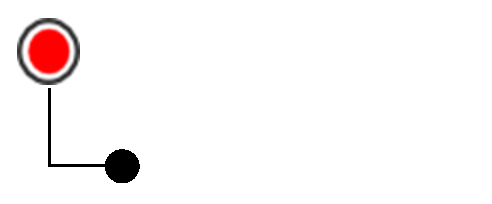
\includegraphics[scale=0.5]{img/kropki.eps}
	\end{center}
\end{wrapfigure}

\textbf{{\LARGE \nazwa}} \\
\linebreak
\textbf{ {\indent \indent \LARGE specification}}\\
\vskip 0.8 true in

\begin{figure}[htbp!]
	\centering
	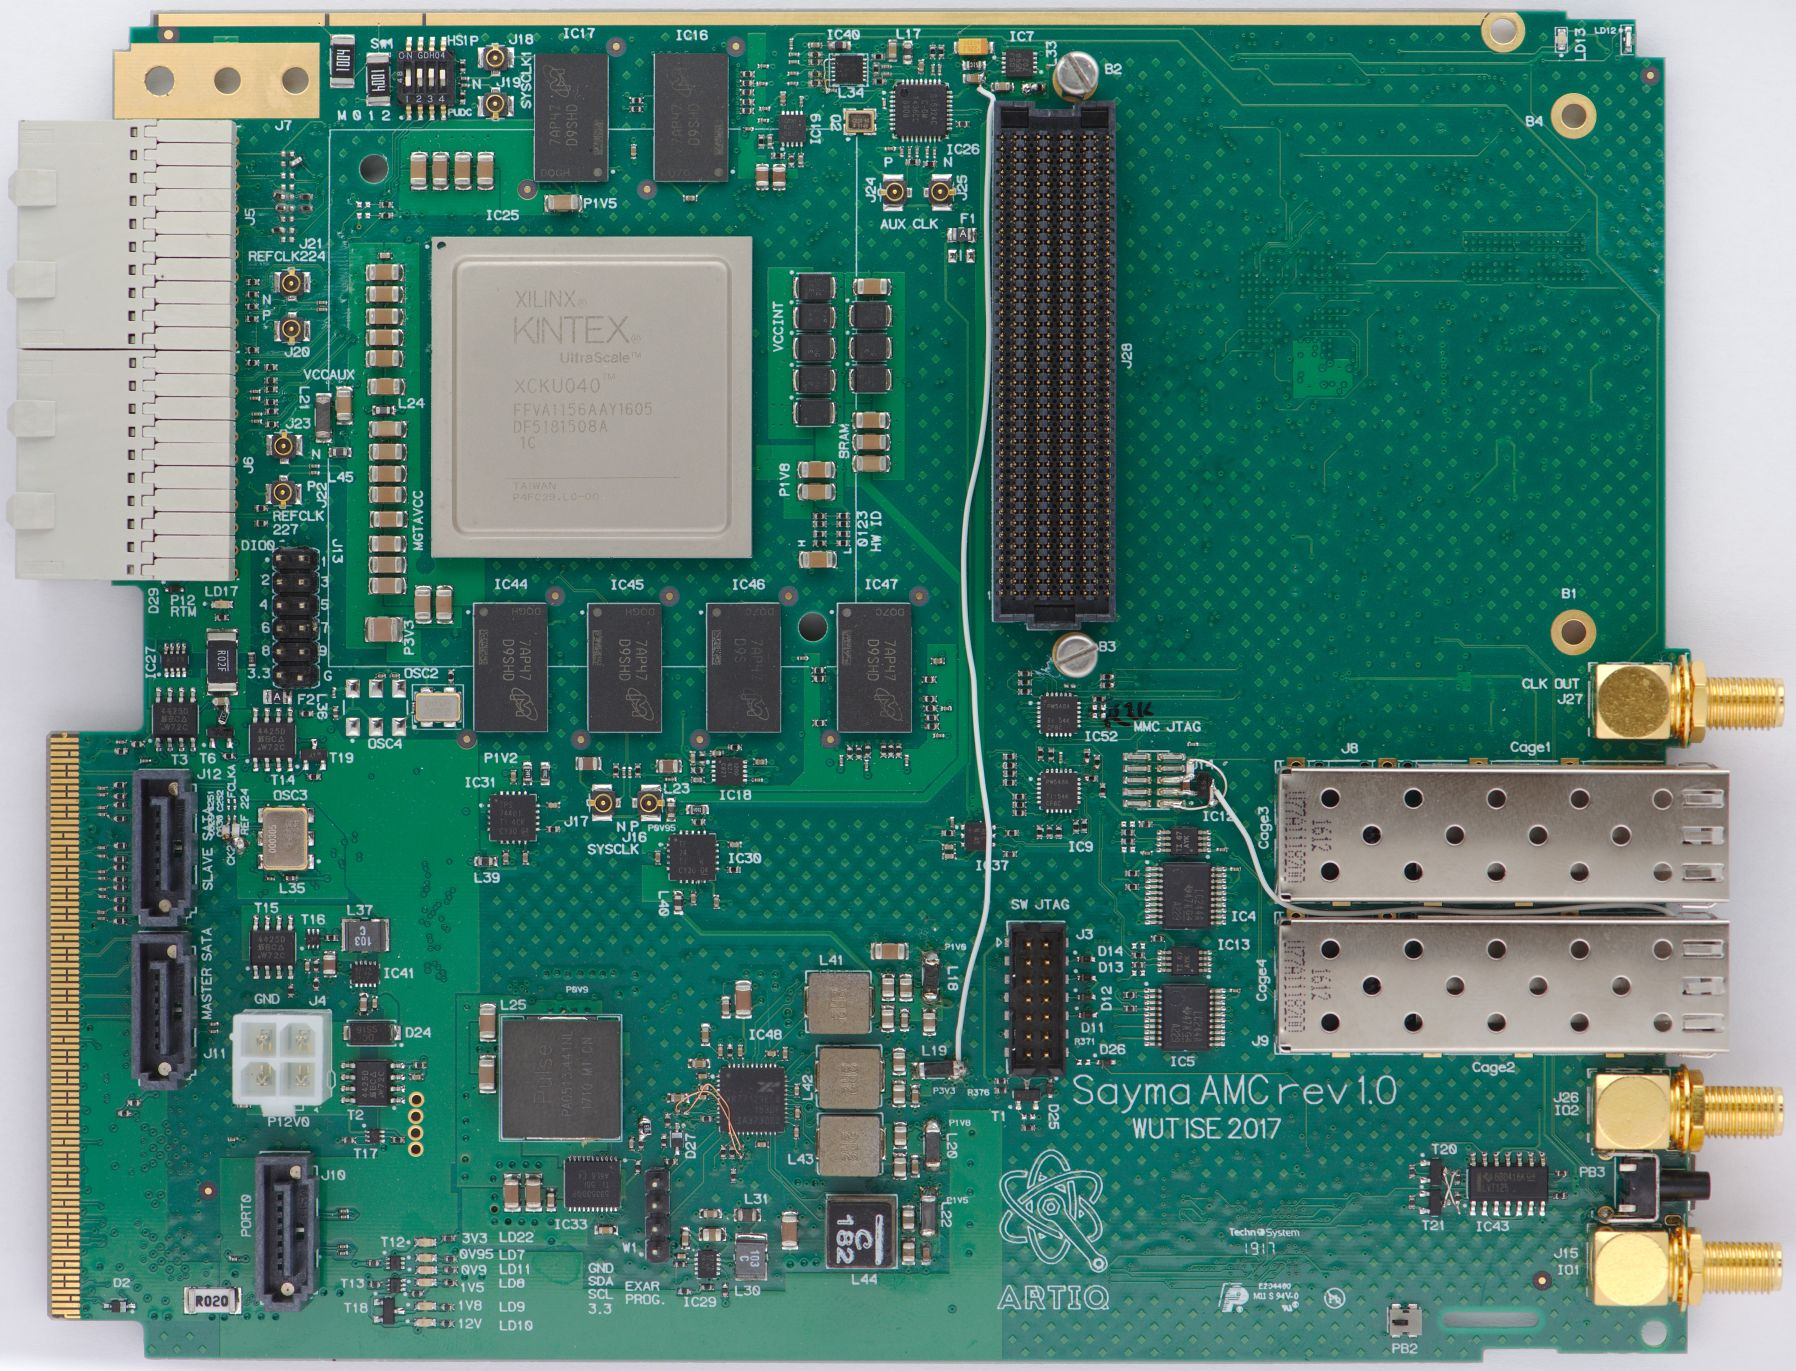
\includegraphics[height=10cm]{img/SaymaT.jpg}\\
	%	\caption{v3.1(02.2017)}
\end{figure}
\begin{center}
	v1.0(11.2017)
\end{center}

\vskip 0.7 true in





\end{titlepage}

%\maketitle



\begin{table}[h!]
\vspace{5cm}
	\centering
	\begin{center}
\begin{tabular}{|l|l|}
	\hline
	\textbf{\rule[-2ex]{0pt}{5.5ex} Document version:} & Preliminary   \\ \hline
\textbf{\rule[-2ex]{0pt}{5.5ex} Issue Date:} & \today         \\ \hline
\textbf{\rule[-2ex]{0pt}{5.5ex} Written by:}      &  Filip Świtakowski                       \\ \hline
\textbf{\rule[-2ex]{0pt}{5.5ex} Approved by:}     &         Greg Kasprowicz      \\ \hline
	\textbf{\rule[-2ex]{0pt}{5.5ex} Document title:}  &  \nazwa - specification \\ \hline

\end{tabular} 
\end{center}
\end{table}

\clearpage


\listoftodos
\clearpage
\tableofcontents



\clearpage


\section{Overview}\label{overview}

MicroTCA (uTCA) is Sinara's preferred form-factor for hardware with
high-speed data converters requiring deterministic phase control, such
as the \href{Sayma}{\emph{Sayma}} 2.4 GSPS smart arbitrary waveform
generator (SAWG).

uTCA is a modular, open standard originally developed by the
telecommunications industry. It allows a single rack master -- the Micro
TCA Carrier Hub (MCH) -- to control multiple slave boards, known as
Advanced Mezzanine Cards (AMCs) via a high-speed digital backplane. uTCA
chassis and backplanes are available commercially of the shelf (COTS).

We make use of the most recent extension to the uTCA standard, uTCA.4.
Originating in the high-energy and particle physics (HEPP) community,
uTCA.4 introduces rear-transition modules (RTMs) along with a second
backplane for low-noise RF signals (RFBP). Each RTM connects to an AMC
(one RTM per AMC). Typically, the AMCs hold FPGAs and other high-speed
digital hardware, communicating with the MCH via gigabit serial links
over the AMC backplane. The RTMs hold data converters and other
low-noise analog components, controlled by the corresponding AMC. The
RFBP provides low-noise clocks and local oscillators (LOs). The RTMs and
RFBP are screened from the AMCs to minimise interference from the
high-speed digital logic.

\begin{figure}[htbp!]
\centering
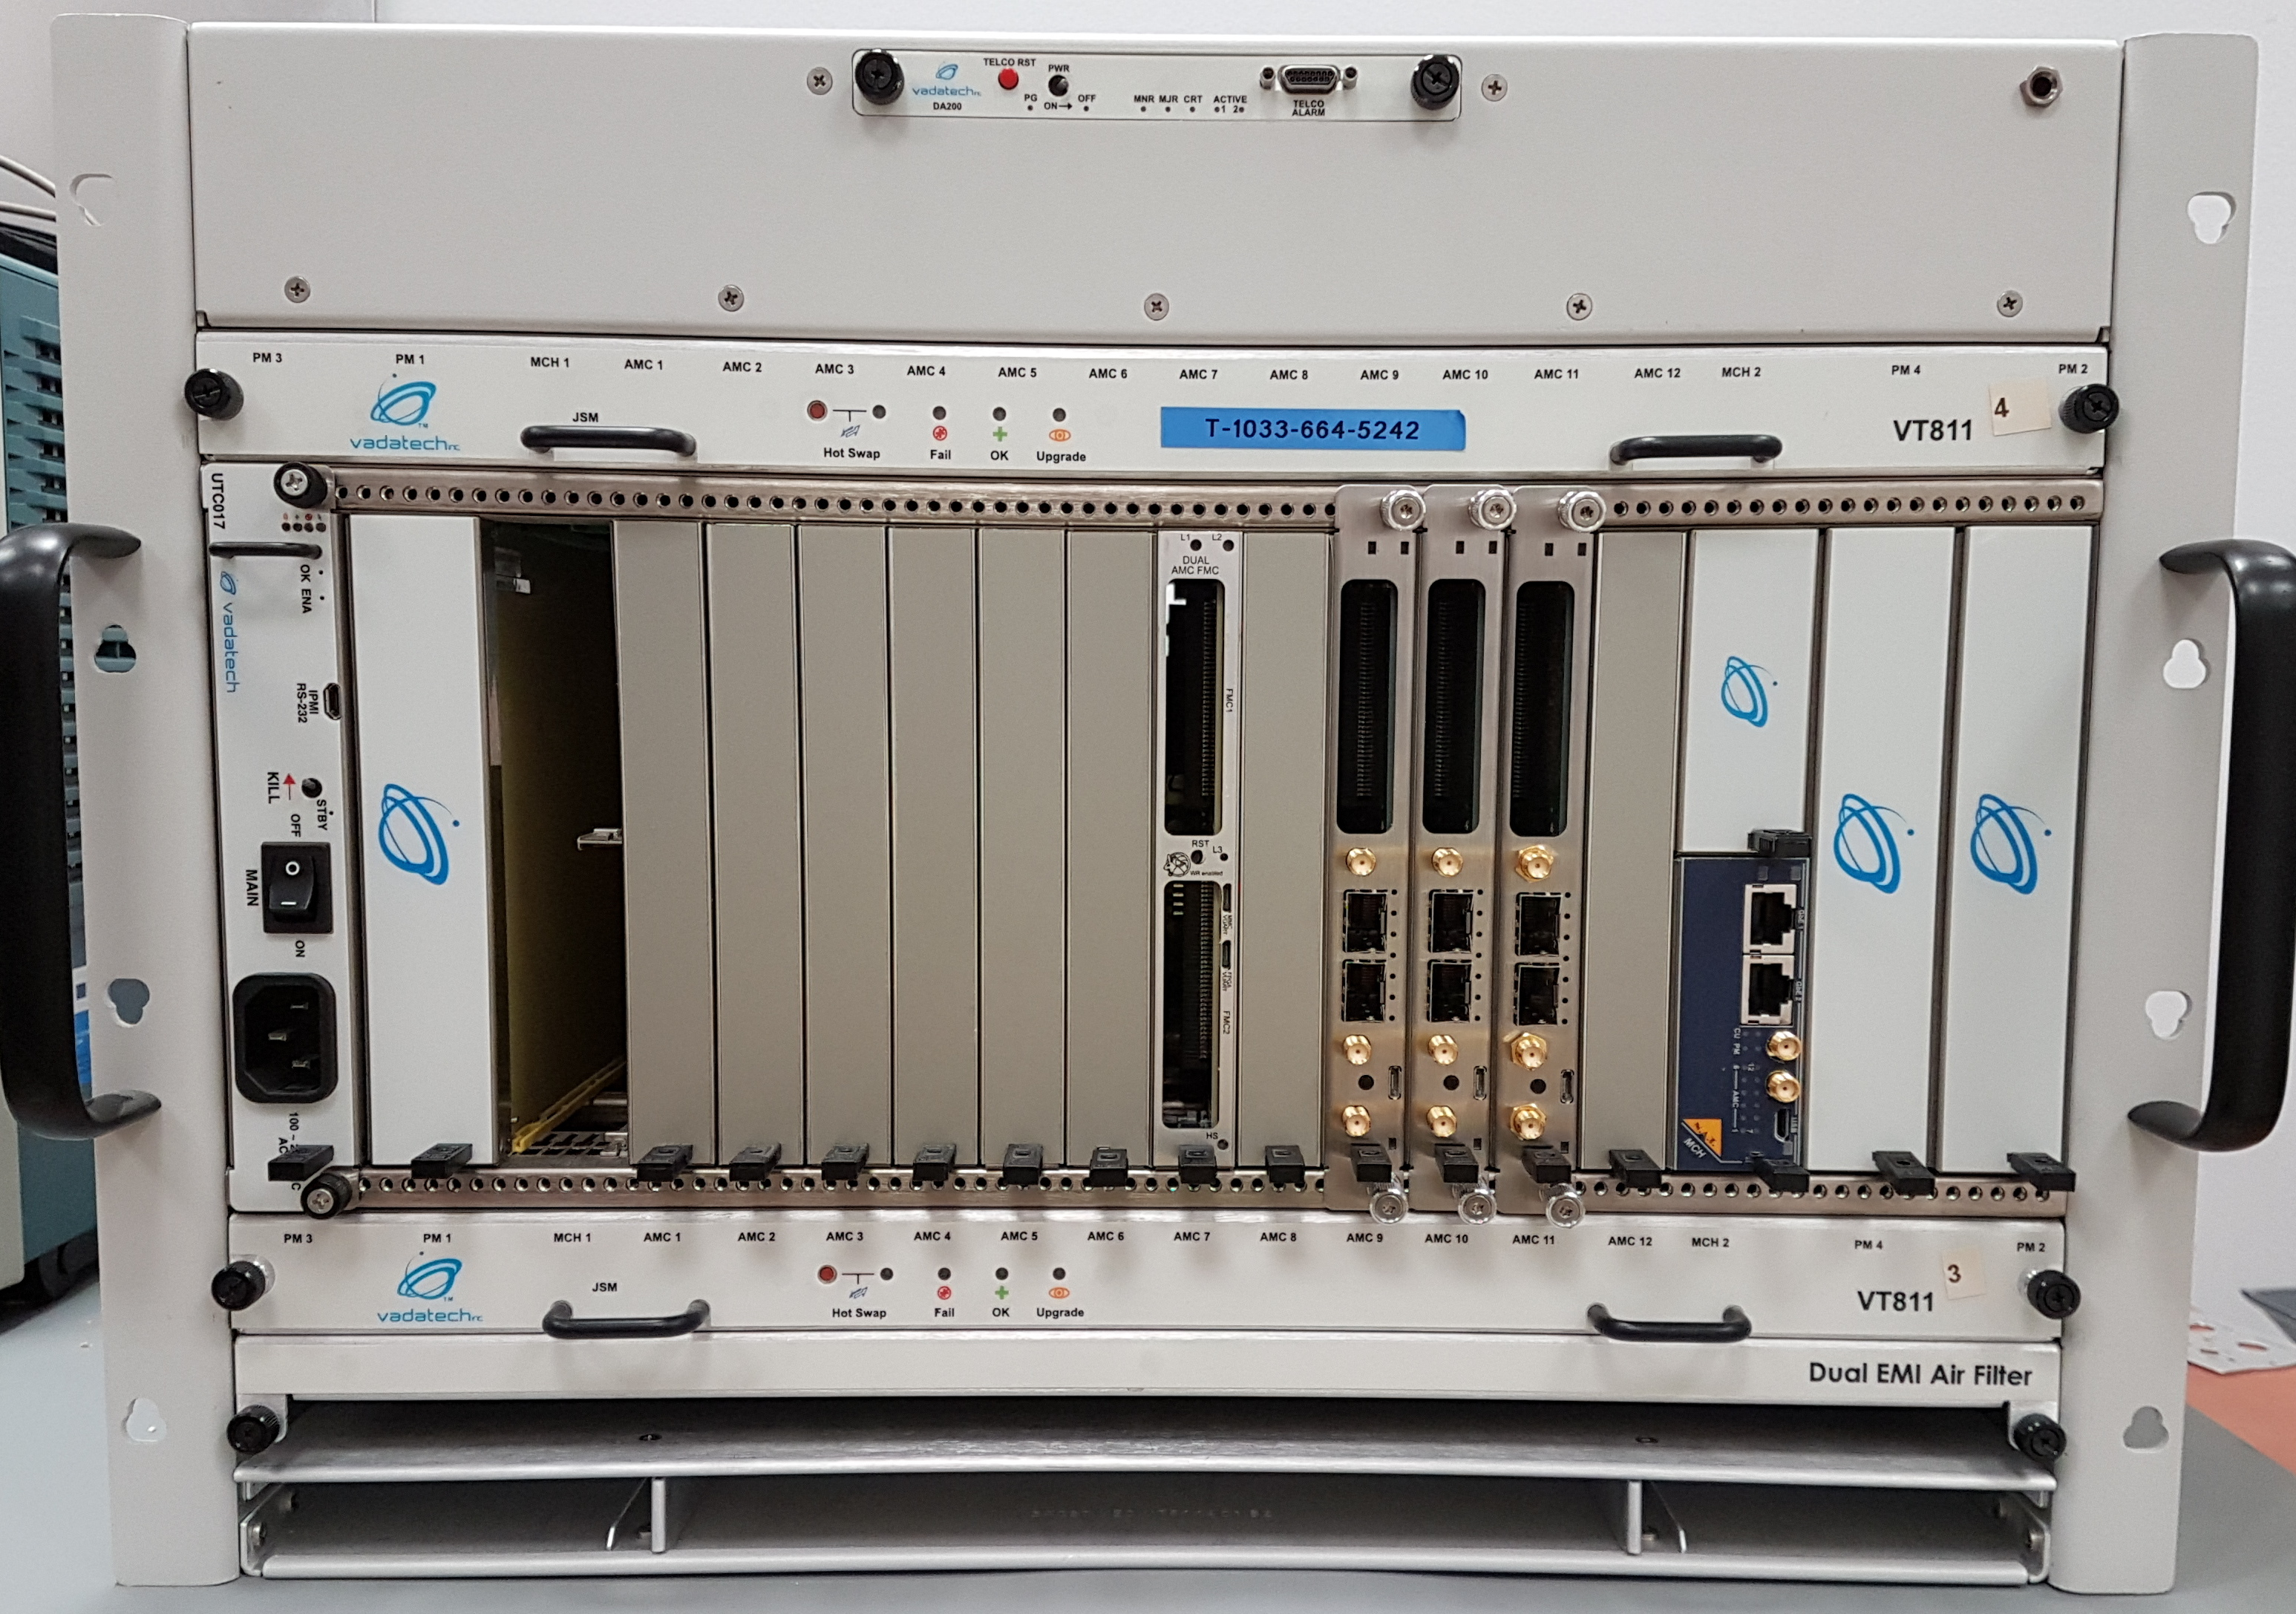
\includegraphics[width=15cm]{img/MTCA_Front.jpg}
\caption{Micro TCA chassis with 3 Sayma AMC modules inserted}
\end{figure}

(above) Micro TCA chassis with 3 Sayma AMC modules inserted.

Micro TCA chassis with 4 RTM modules inserted. One of them with 4
BaseMod AFE mezzanines installed.

\begin{figure}[htbp!]
\centering
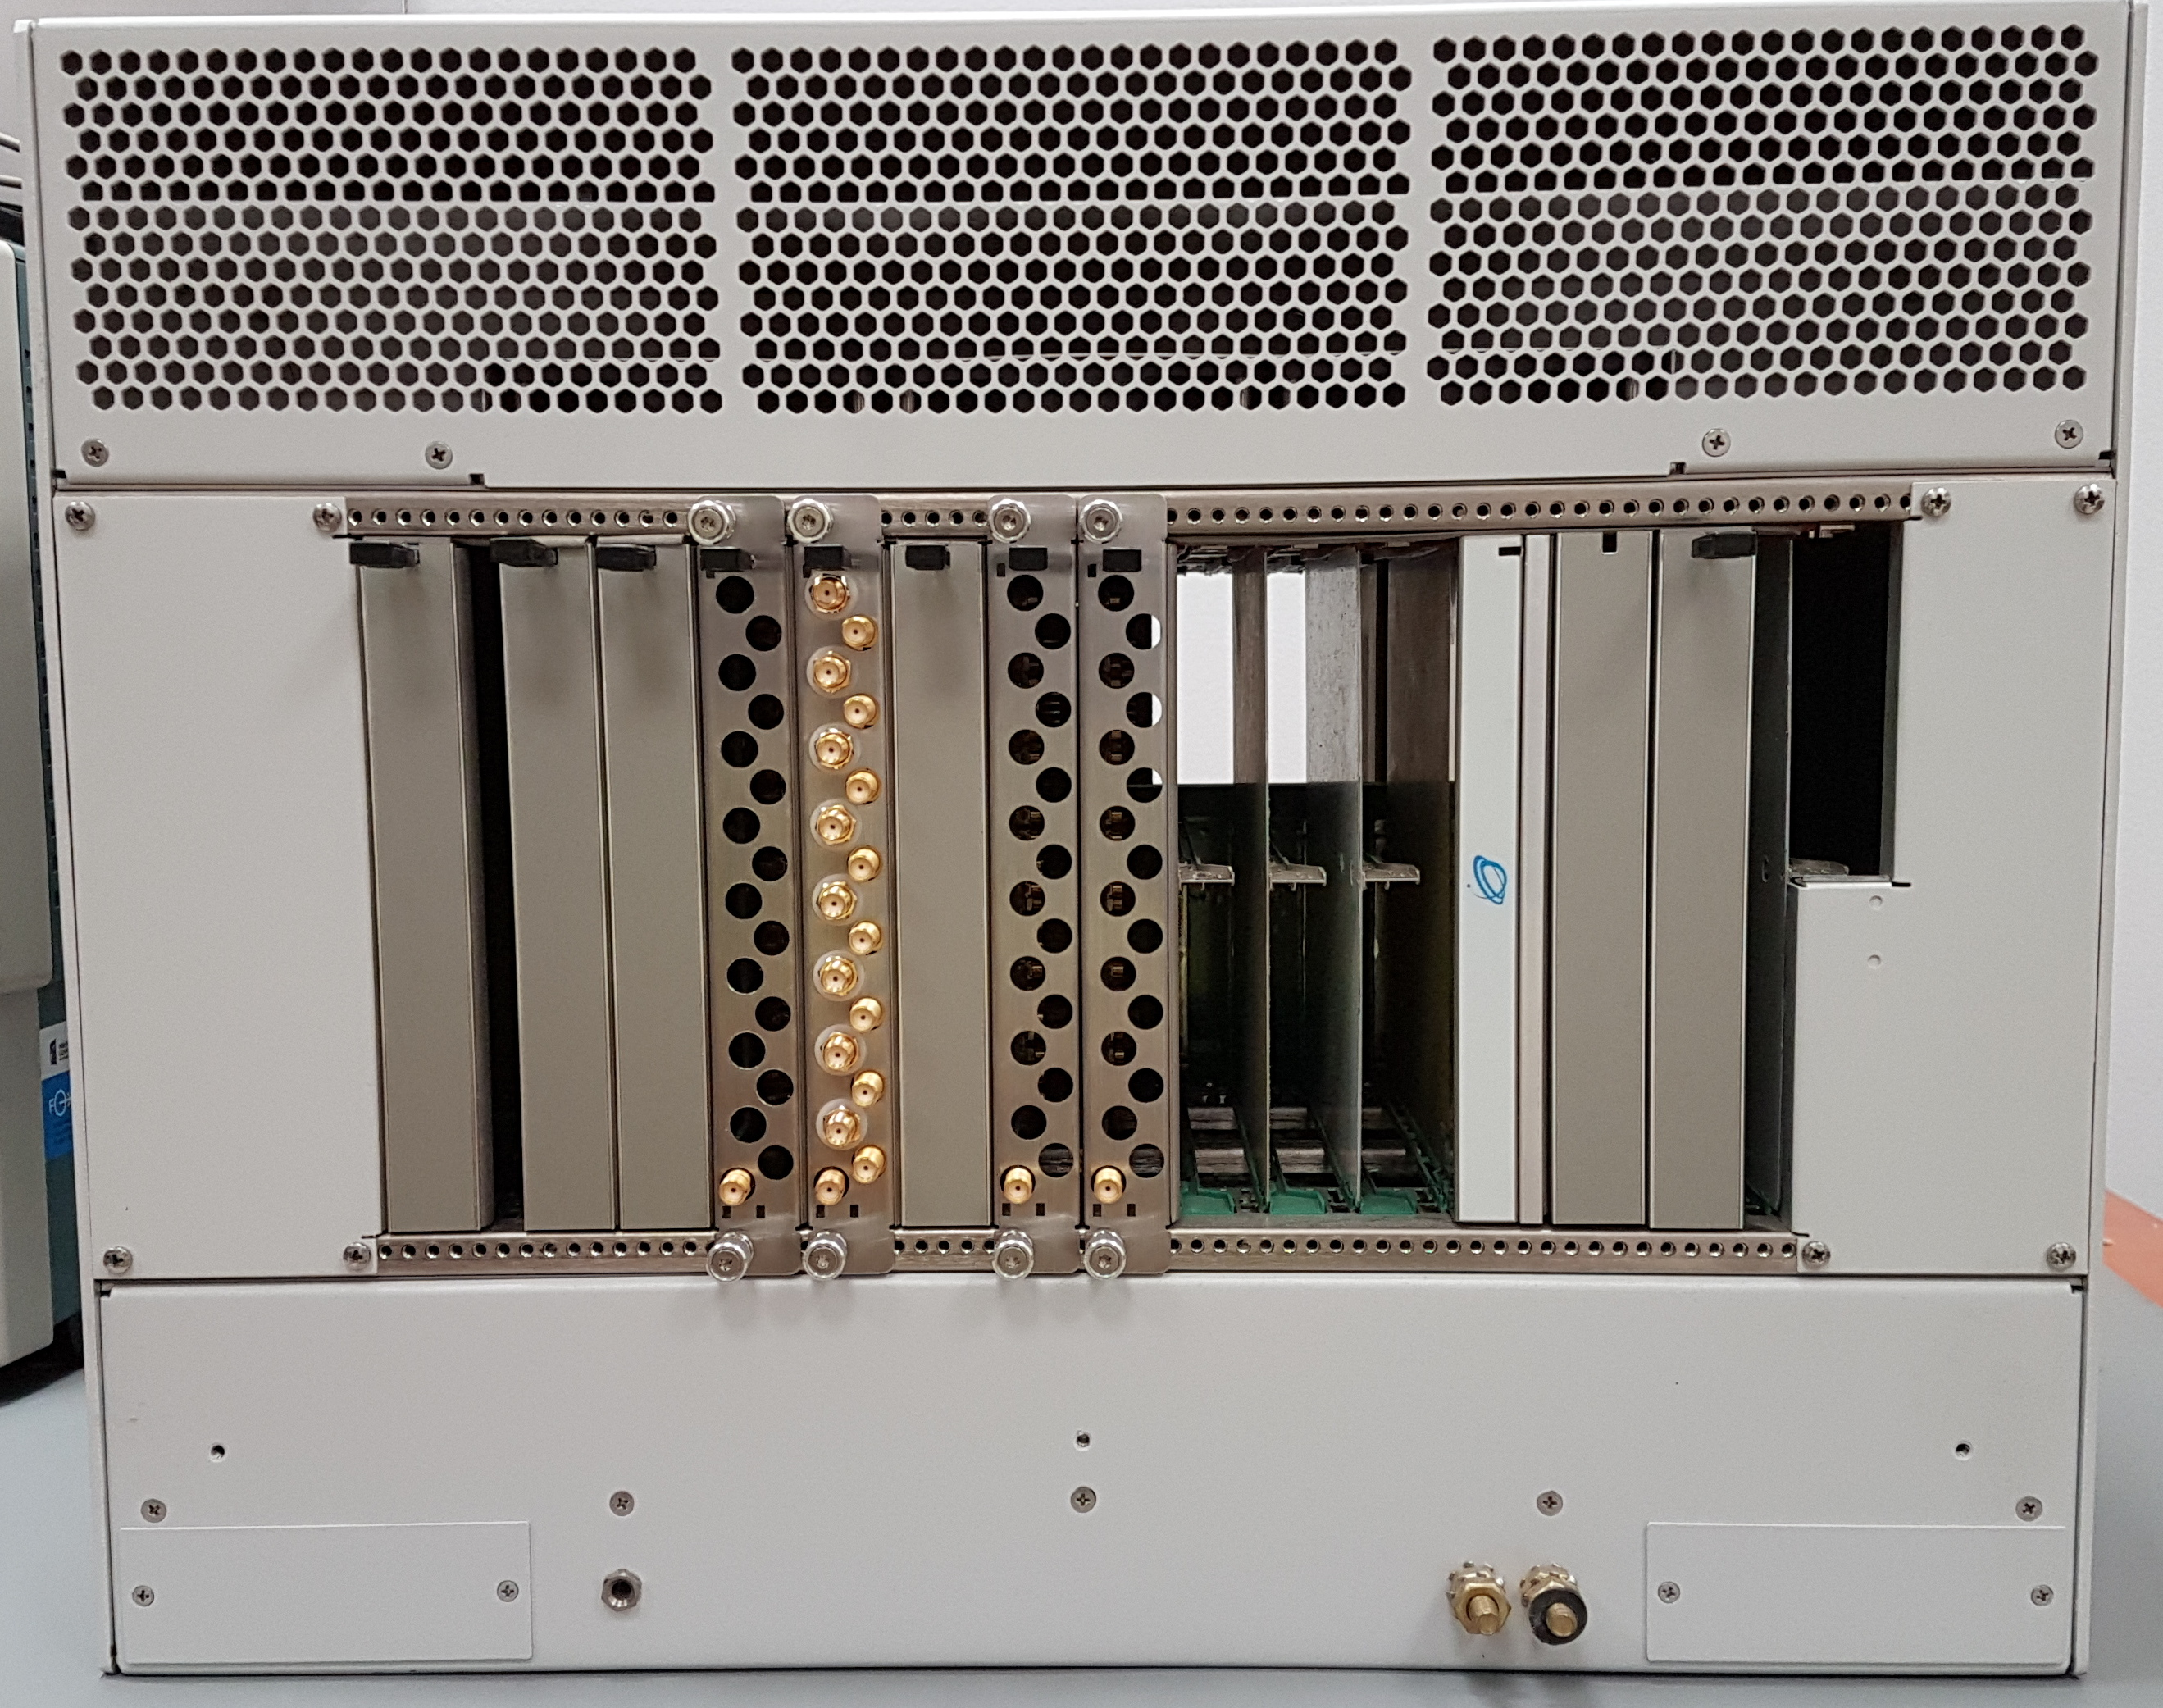
\includegraphics[width=15cm]{img/MTCA_Back.jpg}
\caption{Micro TCA chassis with 4 RTM modules inserted. One of them has
4 BaseMod AFE mezzanines installed.}
\end{figure}

\section{uTCA.4 RF Backplane}\label{utca.4-rf-backplane}

\href{http://mtca.desy.de/sites/site_mtca/content/e172206/e205636/e212584/e248086/uRFB_concept_Datasheet_19.12.2014_eng.pdf}{RF
BP datasheet}
\href{http://ieeexplore.ieee.org/stamp/stamp.jsp?arnumber=7097413\&tag=1}{RF
BP measurements}

\section{uTCA in Sinara}\label{utca-in-sinara}

\href{Metlino}{\emph{Metlino}} has been developed as an MCH optimised
for use in Sinara. It can either be the ARTIQ master or a slave,
connected to the master via DRTIO.

uTCA hardware interfaces with the extension modules either directly,
using a \href{VHDCICarrier}{VHDCI carrier}, or indirectly, using a Kasli
DRTIO slave.

To do: * Some images to illustrate what uTCA systems look like * Explain
how Baikal etc fit in * Add BP schematics that show what the
connectivity is * Any more useful information?

\section{uTCA parts and suppliers}\label{utca-parts-and-suppliers}

Add parts and suppliers from the issues list\ldots{}

\section{Schematic / Layout Viewer}\label{schematic-layout-viewer}

Mentor has a free tool called
\href{https://www.mentor.com/pcb/downloads/visecad-viewer/}{visECAD
Viewer}.

\clearpage

\section{Sayma Smart Arbitrary Waveform
Generator}\label{sayma-smart-arbitrary-waveform-generator}

Sayma is a smart arbitrary waveform generator, providing 8 channels of
1.2 GSPS 16-bit DACs (2.4 GHz DAC clock) and 125 MSPS 16-bit ADCs. It
consists of an AMC, providing the high-speed digital logic, and a RTM,
holding the data converters and analog components.

The design files are located in
\href{https://github.com/m-labs/sinara/tree/master/ARTIQ_EE/PCB_Sayma_AMC}{ARTIQ\_EE/PCB\_Sayma\_AMC}
and
\href{https://github.com/m-labs/sinara/tree/master/ARTIQ_EE/PCB_Sayma_RTM}{ARTIQ\_EE/PCB\_Sayma\_RTM}
and, the AMC schematic is
\href{https://github.com/m-labs/sinara/blob/master/ARTIQ_EE/Sayma_AMC.pdf}{here}
and the RTM schematic is
\href{https://github.com/m-labs/sinara/blob/master/ARTIQ_EE/Sayma_RTM.pdf}{here}.
The PCBs are double width, mid height AMC module. Sayma AMC

\subsection{Features}\label{features}

\begin{itemize}

\item
  May be used in a uTCA rack or stand-alone operation with fibre-based
  DRTIO link
\item
  Analog input and output front-ends provided by plug-in
  \href{SaymaAFE}{analog front-end modules} (eg BaseMod) for maximum
  flexibility.
\item
  Extremely flexible \href{SinaraClocking}{clocking options}
\item
  Flexible feedback to SAWG parameters planned. Specification
  \href{Servo}{here}.
\end{itemize}

\subsection{Key AMC Components}\label{key-amc-components}

\begin{itemize}

\item
  \textbf{FPGA}: XCKU040-1FFVA1156C Kintex Ultrascale, 520 I/O, 530K
  Logic Cells, Speed Grade 1, 20 GTH transceivers (up to 16.3 Gb/s) --
  motivation for this FPGA choice is
  \href{https://github.com/m-labs/sinara/wiki/artiq_hardware\#recommendation}{here}
\item
  \textbf{DRAM}: MT41K256M16TW-107:P, DDR3, 32 MB x 16 x 8 banks = 4 GB
\item
  \textbf{clock recovery}: Si5324 is a precision clock multiplier and
  jitter attenuator
\end{itemize}

\subsection{Key RTM Components}\label{key-rtm-components}

\begin{itemize}

\item
  \textbf{DAC}: AD9154 4-channel high-speed data converter

  \begin{itemize}

  \item
    data rate is 1.2 GS/s at 16-bit
  \item
    clock is up to 2.4 GHz (1x, 2x, 4x and 8x interpolating modes)
  \item
    supports mix-mode to emphasize power in 3rd Nyquist Zone
  \item
    interface is 8-lane JESD204B (subclass 1)
  \item
    power consumption is 2.11 W
  \item
    each Sayma has 2 AD9154
  \end{itemize}
\item
  \textbf{ADC}: AD9656 is a 4-channel high-speed digitizer

  \begin{itemize}

  \item
    data rate is 125 MS/s at 16-bit
  \item
    clock is up to 125 MHz
  \item
    650 MHz analog bandwidth
  \item
    interface is 8-lane, 8 Gb/s per lane, JESD204B (subclass 1)
  \item
    each Sayma has 2 AD9656
  \end{itemize}
\item
  \textbf{clock generation}: (summarized \href{SinaraClocking}{here})

  \begin{itemize}

  \item
    Sayma has several distinct clock domains

    \begin{itemize}

    \item
      DAC, JESB204B output clock
    \item
      ADC, JESD204B input clock
    \item
      LO for analog mezzanines
    \end{itemize}
  \item
    These clocks may be generated using a low phase noise
    \href{ClockMezzanines}{Clock Mezzanine} PCB. A single Clock
    Mezzanine can be shared by several Sayma in a uTCA crate using
    {[}Baikal{]} PCB and an RTM RF backplane. Alternately, each Sayma
    can have its own distinct Clock Mezzanine (local generation).
  \end{itemize}
\item
  \textbf{clock distribution}

  \begin{itemize}

  \item
    HMC7043 SPI 14-Output Fanout Buffer for JESD204B
  \item
    HMC830 SPI fractional-N PLL
  \end{itemize}
\item
  \textbf{calibration ADC}: AD7194BCPZ is a 20-bit ADC for
  monitoring/calibration
\end{itemize}

\subsection{Transceiver/connector
usage}\label{transceiverconnector-usage}

\begin{itemize}

\item
  SFP1: DRTIO downstream
\item
  SFP2: DRTIO downstream
\item
  SATA1: DRTIO upstream (different bitstream probably)
\item
  SATA2 (swapped): DRTIO downstream
\item
  FAT\_PIPE1 (FABRICD): DRTIO upstream
\item
  FAT\_PIPE2 (FABRICE): not used
\item
  FMC:
\item
  LA: FMC DIO32: TTL IO
\end{itemize}



\clearpage

%\section{Introduction to Micro TCA}




%The MTCA platform is available on the market for over
%ten years. It evolved from telecommunication ATCA standard. The MTCA sandard utilizes ATCA-defined AMC boards
%used directly in dedicated chassis. It also defines MTCA
%Carrier Hub (MCH) which controlls multiple slave boards, known as Advanced Mezzanine Cards (AMCs) via a high-speed digital backplane. AMC card can be equipped with FPGA Mzzanine Cards (FMCs) which are I/O modules pluggable to High-pin Count (HPC) or Low-pin Count (LPC) connector. 
%
%%which consists of Ethernet hub and crate
%%management system. 
%The MTCA crates are available in several
%form-factors for industrial, aviation and military use.
%User can easily extend and adopt the standard to particular application by selection of
%proper chassis, cooling method, computing and connectivity
%technology while keeping same mechanical, electrical standard and software architecture.\\


%MicroTCA (uTCA) is Sinara's preferred form-factor for hardware with high-speed data converters requiring deterministic phase control, such as the Sayma 2.4GSPS smart arbitrary waveform generator (SAWG).
%
%uTCA is a modular, open standard originally developed by the telecommunications industry. It allows a single rack master -- the Micro TCA Carrier Hub (MCH) -- to control multiple slave boards, known as Advanced Mezzanine Cards (AMCs) via a high-speed digital backplane. uTCA chassis and backplanes are available commercially of the shelf (COTS).
%%
%We make use of the most recent extension to the uTCA standard, uTCA.4. Originating in the high-energy and particle physics (HEPP) community, uTCA.4 introduces rear-transition modules (RTMs) along with a second backplane for low-noise RF signals (RFBP). Each RTM connects to an AMC (one RTM per AMC). Typically, the AMCs hold FPGAs and other high-speed digital hardware, communicating with the MCH via gigabit serial links over the AMC backplane. The RTMs hold data converters and other low-noise analog components, controlled by the corresponding AMC. The RFBP provides low-noise clocks and local oscillators (LOs). The RTMs and RFBP are screened from the AMCs to minimise interference from the high-speed digital logic

\section{Glossary}

\begin{description}
	\item[AMC Module or Modul] An AMC Module is a mezzanine or modular add-on card that extends the
	functionality of a Carrier Board. The term is also used to generically refer to the
	different varieties of Multi-Width and Multi-Height Modules.
	\item[Fat Pipes] Ports 4 though 11 of the AMC Connector constitute the Fat Pipes Region. This
	Region of Ports is intended for the assignment of multiple Lane interfaces, also
	called “fat pipes”. Fat Pipe 1 [Ports 4-7], Fat Pipe [Ports 8-11].
	\item[FMC] FPGA Mezzanine Card
	\item[Hot Swap] To remove a component (e.g., an AMC Module) from a system (e.g., an AMC Carrier
	AdvancedTCA Board) and plug in a new one while the power is still on and the
	system is still operating.
	\item[Management Power or MP] The 3.3V power for a Module's Management function, individually provided to each Slot by the Carrier
	\item[IPMB] ntelligent Platform Management Bus. The lowest level hardware management bus
	as described in the Intelligent Platform Management Bus Communications Protocol
	Specification.
	\item[MGT] Multi-Gigabit Transceiver
	\item[MMC] Module Management Controller. The MMC is the required intelligent controller that
	manages the Module and is interfaced to the Carrier via IPMB-Local
	\item[RTM] Rear Transition Module
\end{description}



\clearpage


%\section{Project description}
%	
%The Sayma AMC is a Advanced Mezzanine Card carrier board to carry FMC cards and connect RTM modules.
%
%	

\section{Functional specifications}

\noindent

\textbf{Programmable resources:}

\begin{itemize}
\item Xilinx Kintex UltraScale – XCKU040-1FFVA-1156C    FPGA
	\begin{itemize}
		\item speed grade: -1
		\item 20 GTH transceivers (Max Preformance 16.3 Gb/s)
	\end{itemize}
\item MMC: LPC17762984
\end{itemize}	

\textbf{Memory:}

\begin{itemize}
	\item 512Mb  DDR3 SDRAM (32-bit interface), 800MHz (clock)
	\item 1Gb  DDR3 SDRAM (64-bit interface), 800MHz (clock)
	\item SPI Flash for FPGA configuration. Accessible by MMC
	\item SPI Flash for user data storage
	\item EEPROM with MAC and unique ID 
	
\end{itemize}

\textbf{Connectivity:}

\begin{itemize}
	\item 1 high pin count (HPC) FMC slot for single width mezzanine card
	\item Micro-USB UART connected to FPGA or MMC
	\item Stand-alone 12V power connector 
	\item MGT (Multi-Gigabit Transceiver) connected to:
	\begin{itemize}
%		\item FMC x1
		\item RTM x16
		\item Fat\_Pipe1 x2
%		\item AMC P2P x4
%		\item Port 0 – possibility connected to SATA
		\item SFP x2
	\end{itemize}
%	\item RTM connector with 8 GTP routed to it. Compatible with Sayma RTM module.
	\item  Port 0 – possibility connected to SATA
	\item RTM connector compatible with Sayma RTM module
	
\end{itemize}

\textbf{Supply:}

\begin{itemize}
	\item Monitoring of voltage and Power supply for RTM 12V and FMC 12V
	\item FMC VADJ fixed to 1V8
	\item Monitoring current of all FMC buses
	\item Stand-alone power connectore
%	\item Czy Exar monitoruje powera? 
	
\end{itemize}


\textbf{Clocking:}

\begin{itemize}
	\item Clock recovery Si5324
	\item UFL CLK input
	\item SMA CLK output
 
	
\end{itemize}


\textbf{Other:}

\begin{itemize}
	\item Temperature, voltage and current monitoring for critical power buses
	\item Temperature monitoring: FMC1, supply, FPGA core, DDR memory
	\item JTAG multiplexer (SCANSTA) for FMC access, local JTAG port and remote debug/Chipscope via Ethernet
	
\end{itemize}









\clearpage


\section{Product view}	
	
	\begin{figure}[htbp!]
		\centering
		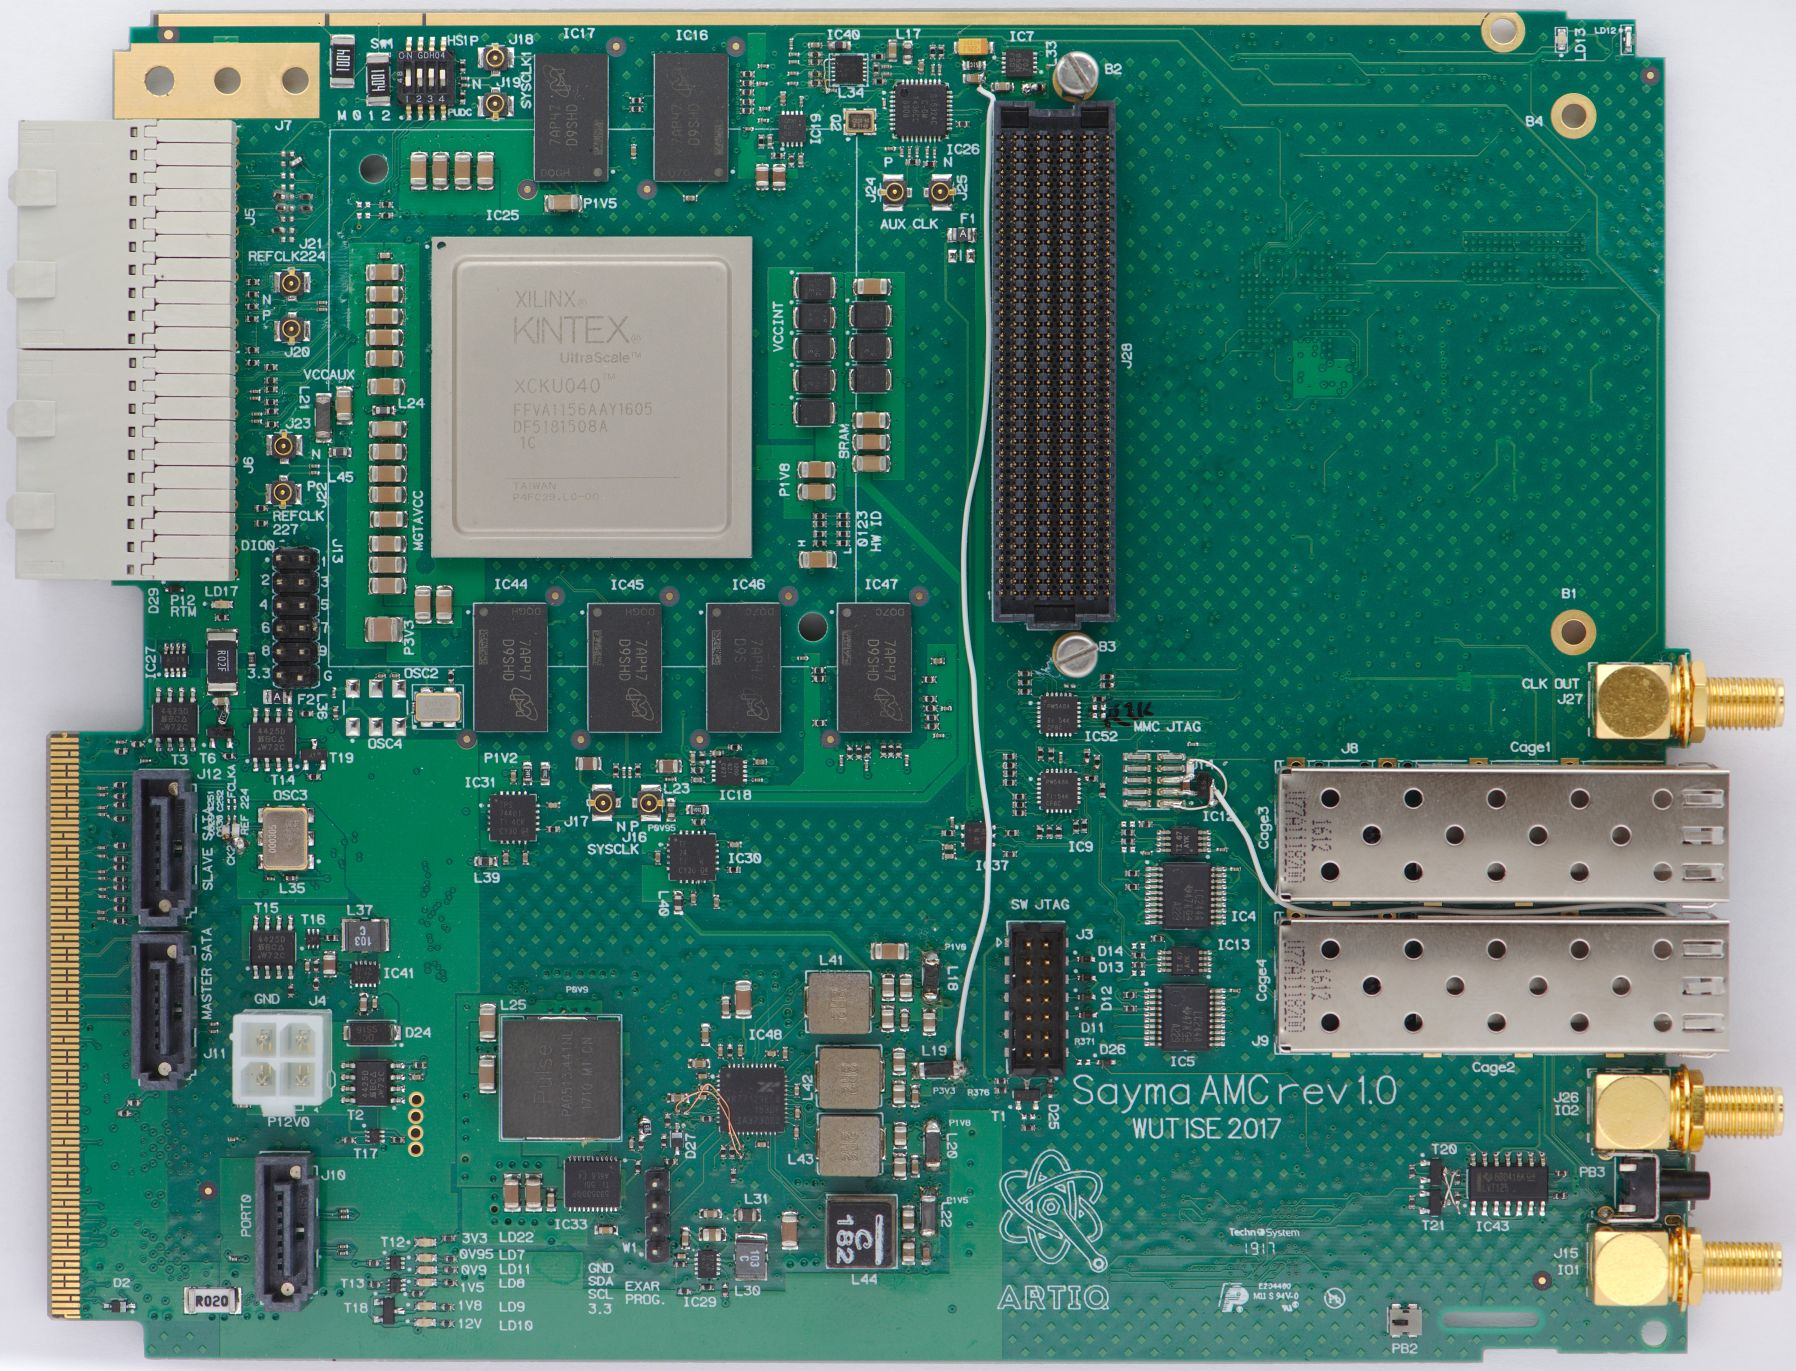
\includegraphics[height=10cm]{img/SaymaT.jpg}\\
		\caption{Top view}
	\end{figure}
	
		\begin{figure}[htbp!]
			\centering
			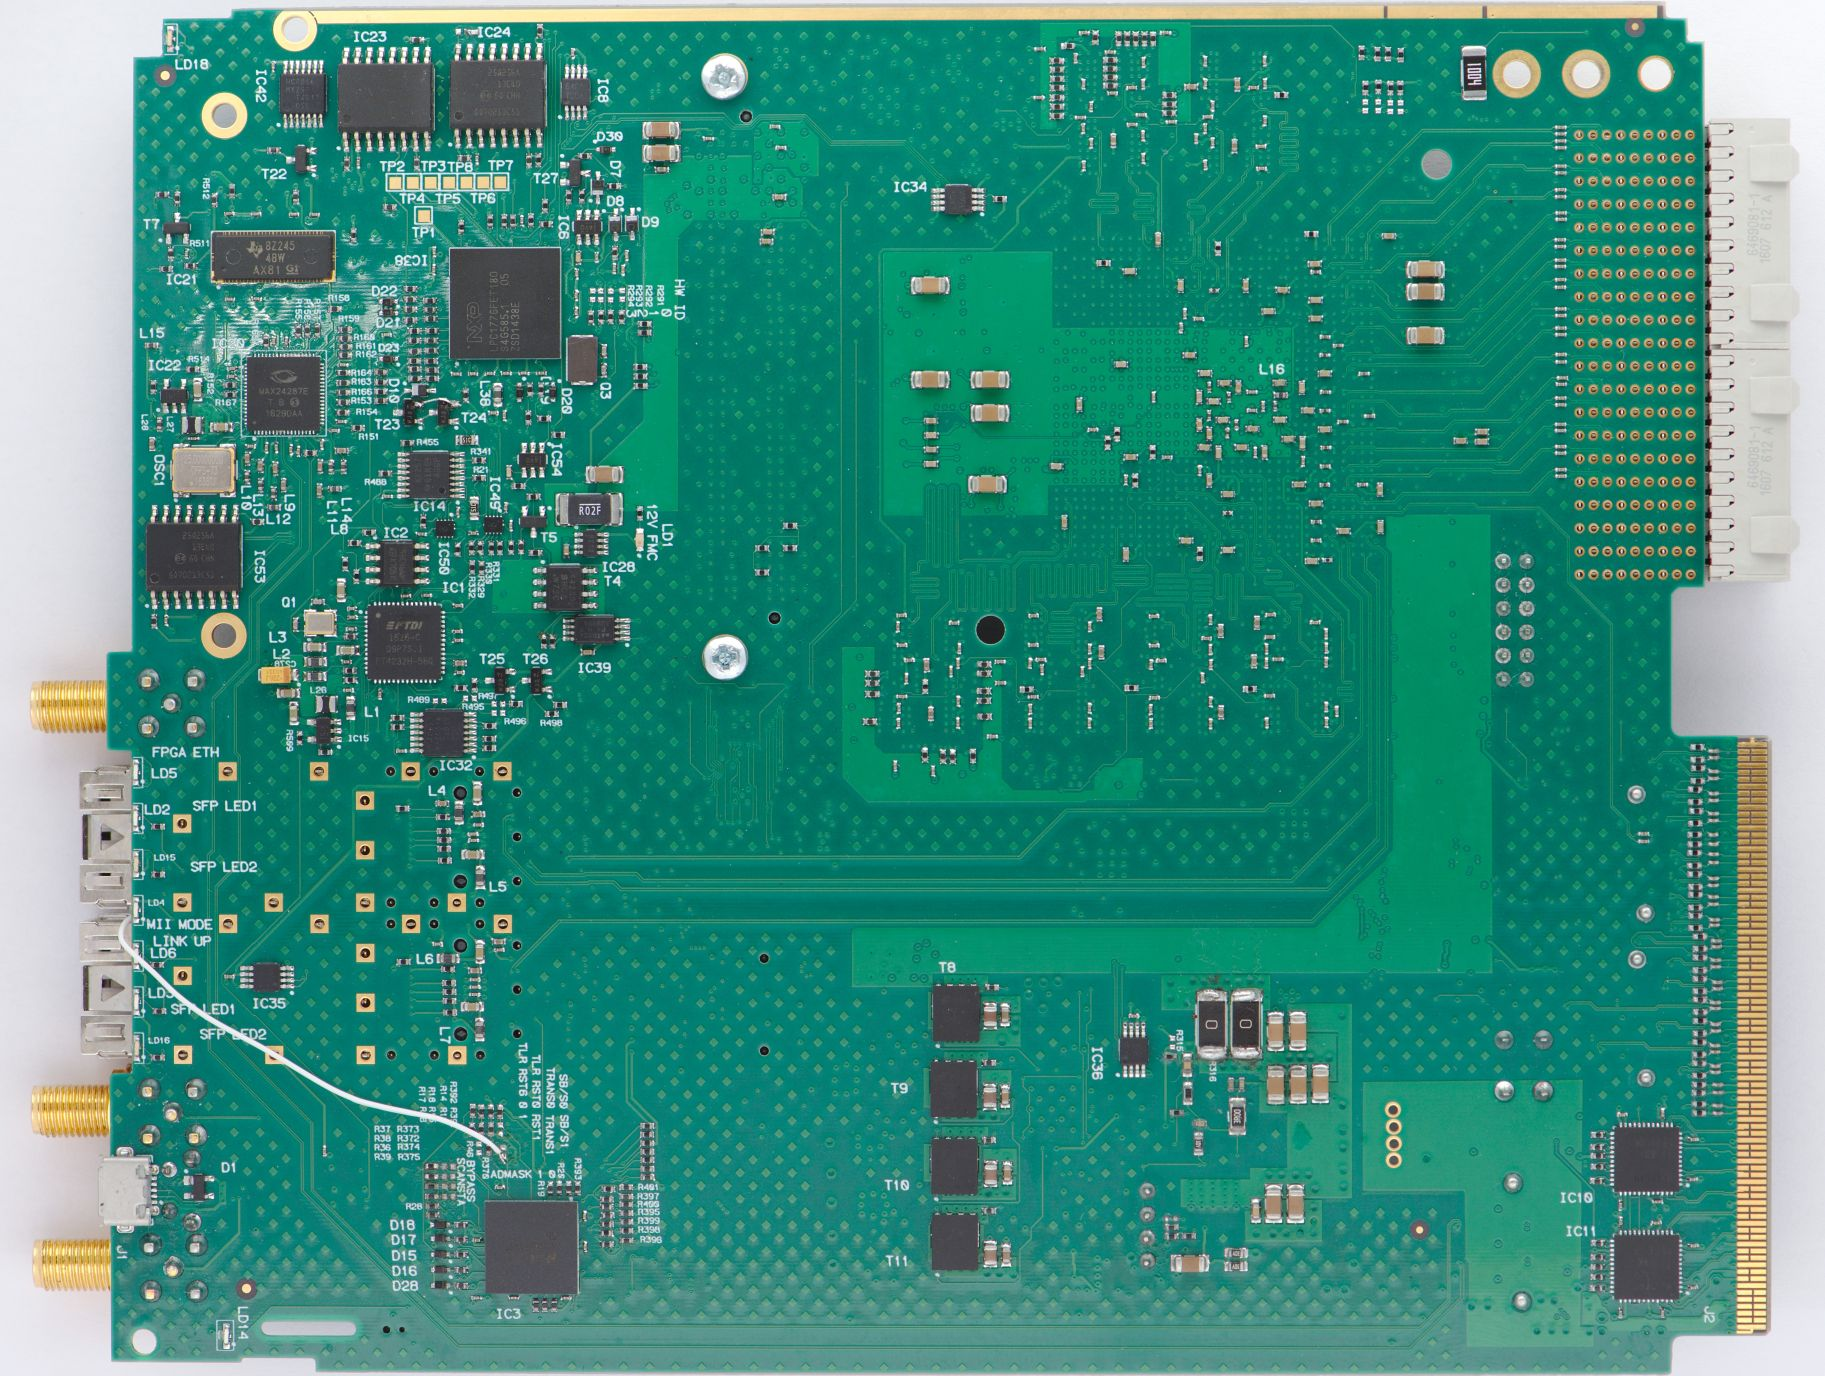
\includegraphics[height=10cm]{img/SaymaB.jpg}\\
			\caption{Bottom view}
		\end{figure}

		\begin{figure}[htbp!]
			\centering
			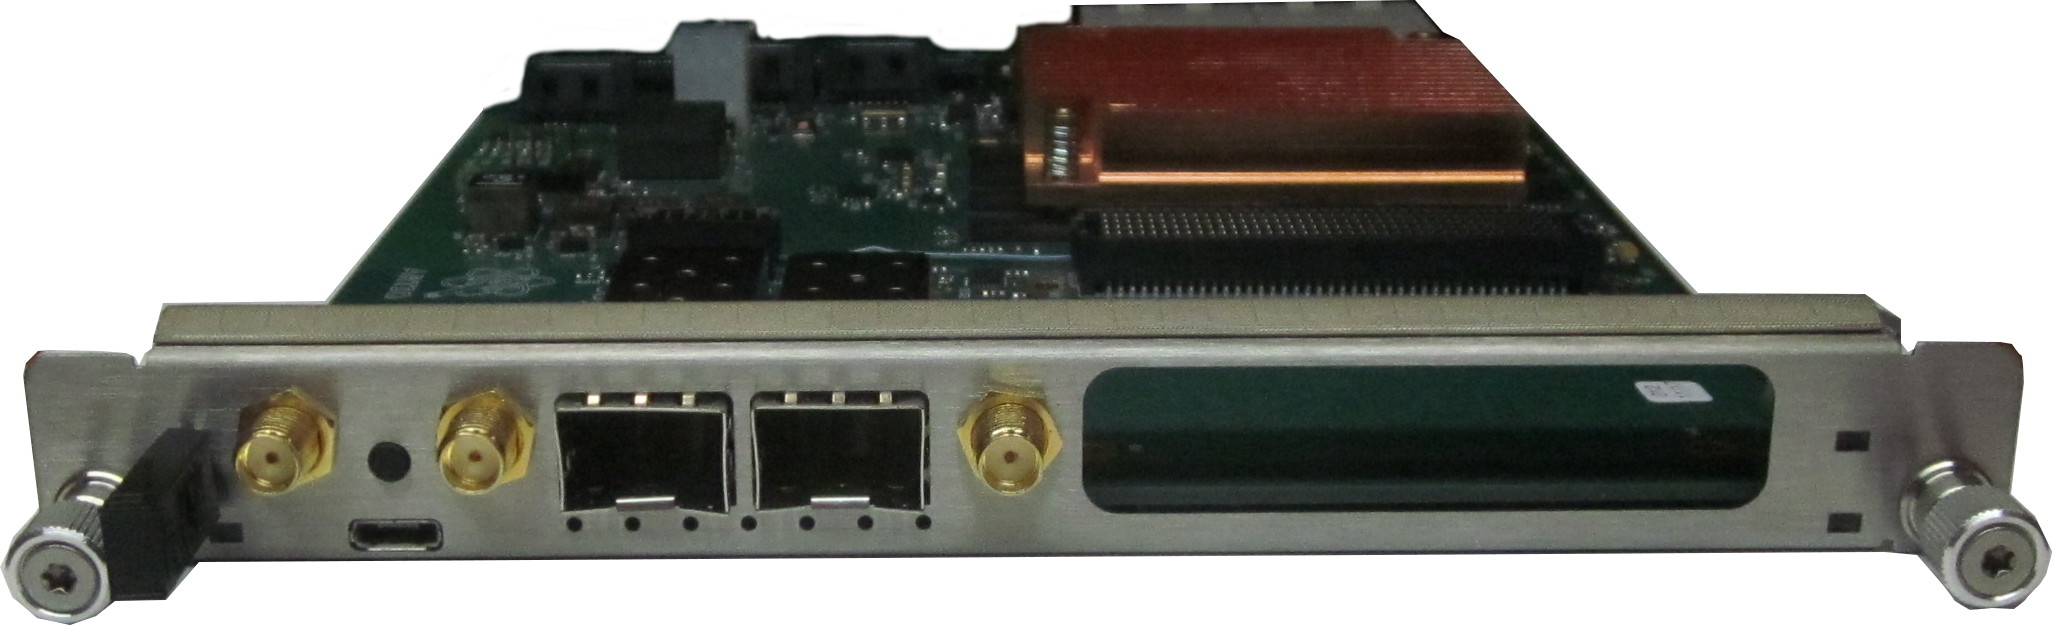
\includegraphics[width=14cm]{img/SaymaF.jpg}\\
			\caption{Front view}
		\end{figure}
	
		\begin{figure}[htbp!]
			\centering
			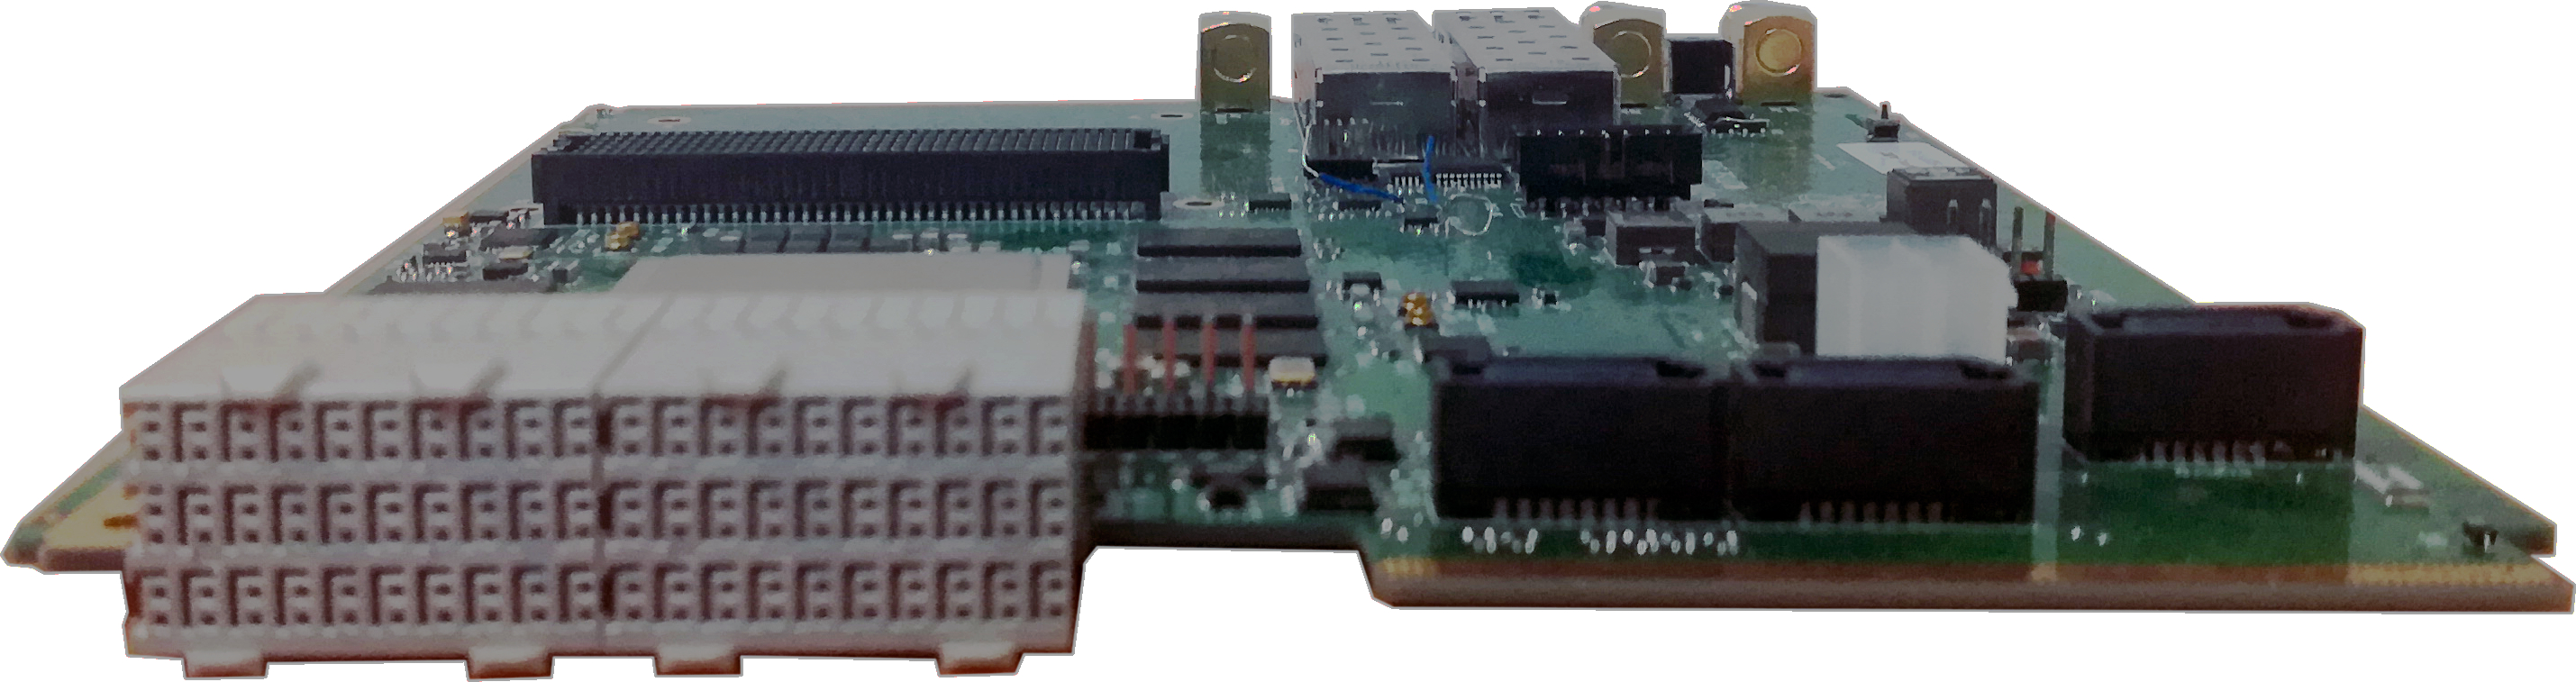
\includegraphics[width=14cm]{img/back.jpg}\\
			\caption{Back view}
		\end{figure}

\clearpage

\section{Routing}


This section contain general bloch scheme of SAYMA AMC board and I2C map with addresses. General Block Scheme -figure \ref{BlockScheme}
shows more importand connections between components. I2C connections with addresses can be found in figure \ref{I2C}. Detailed clocking scheme can be found in next paragraph in figure \ref{clocking}.
	\begin{figure}[htbp!]
		\centering
		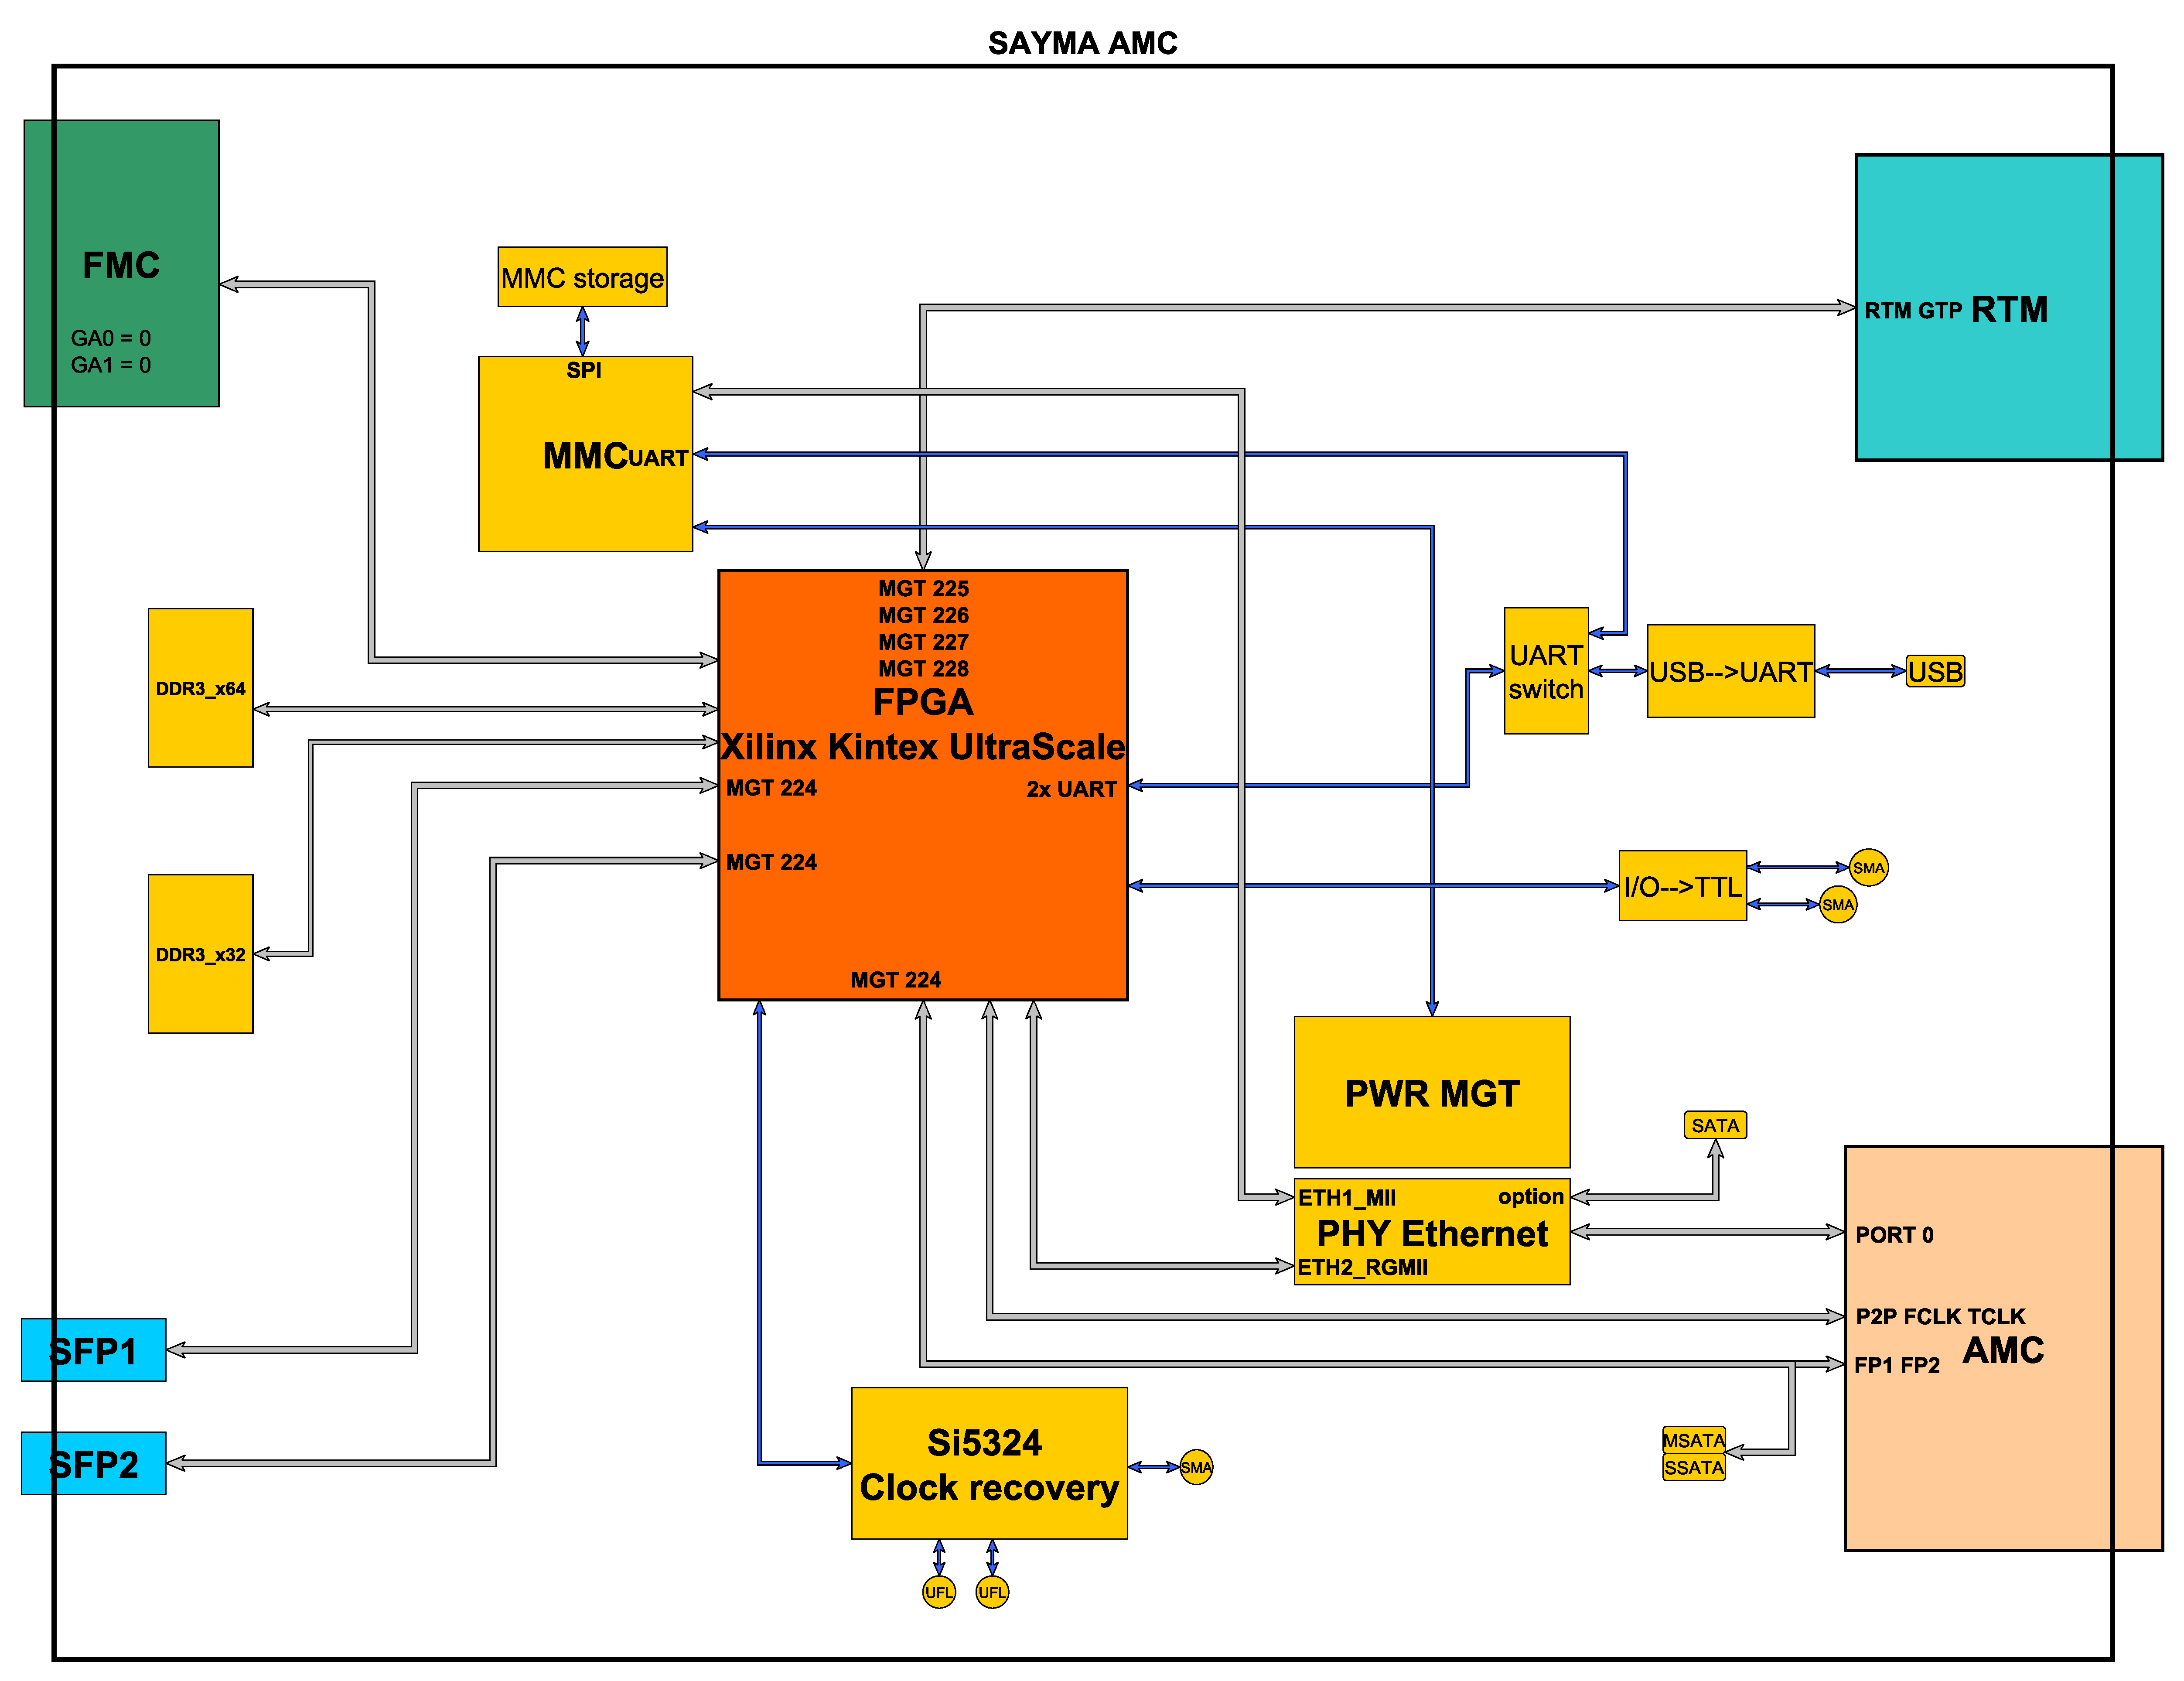
\includegraphics[scale=0.2]{img/sch.eps}\\
		\caption{General Block Scheme}\label{BlockScheme}
	\end{figure}


	\begin{figure}[htbp!]
		\centering
		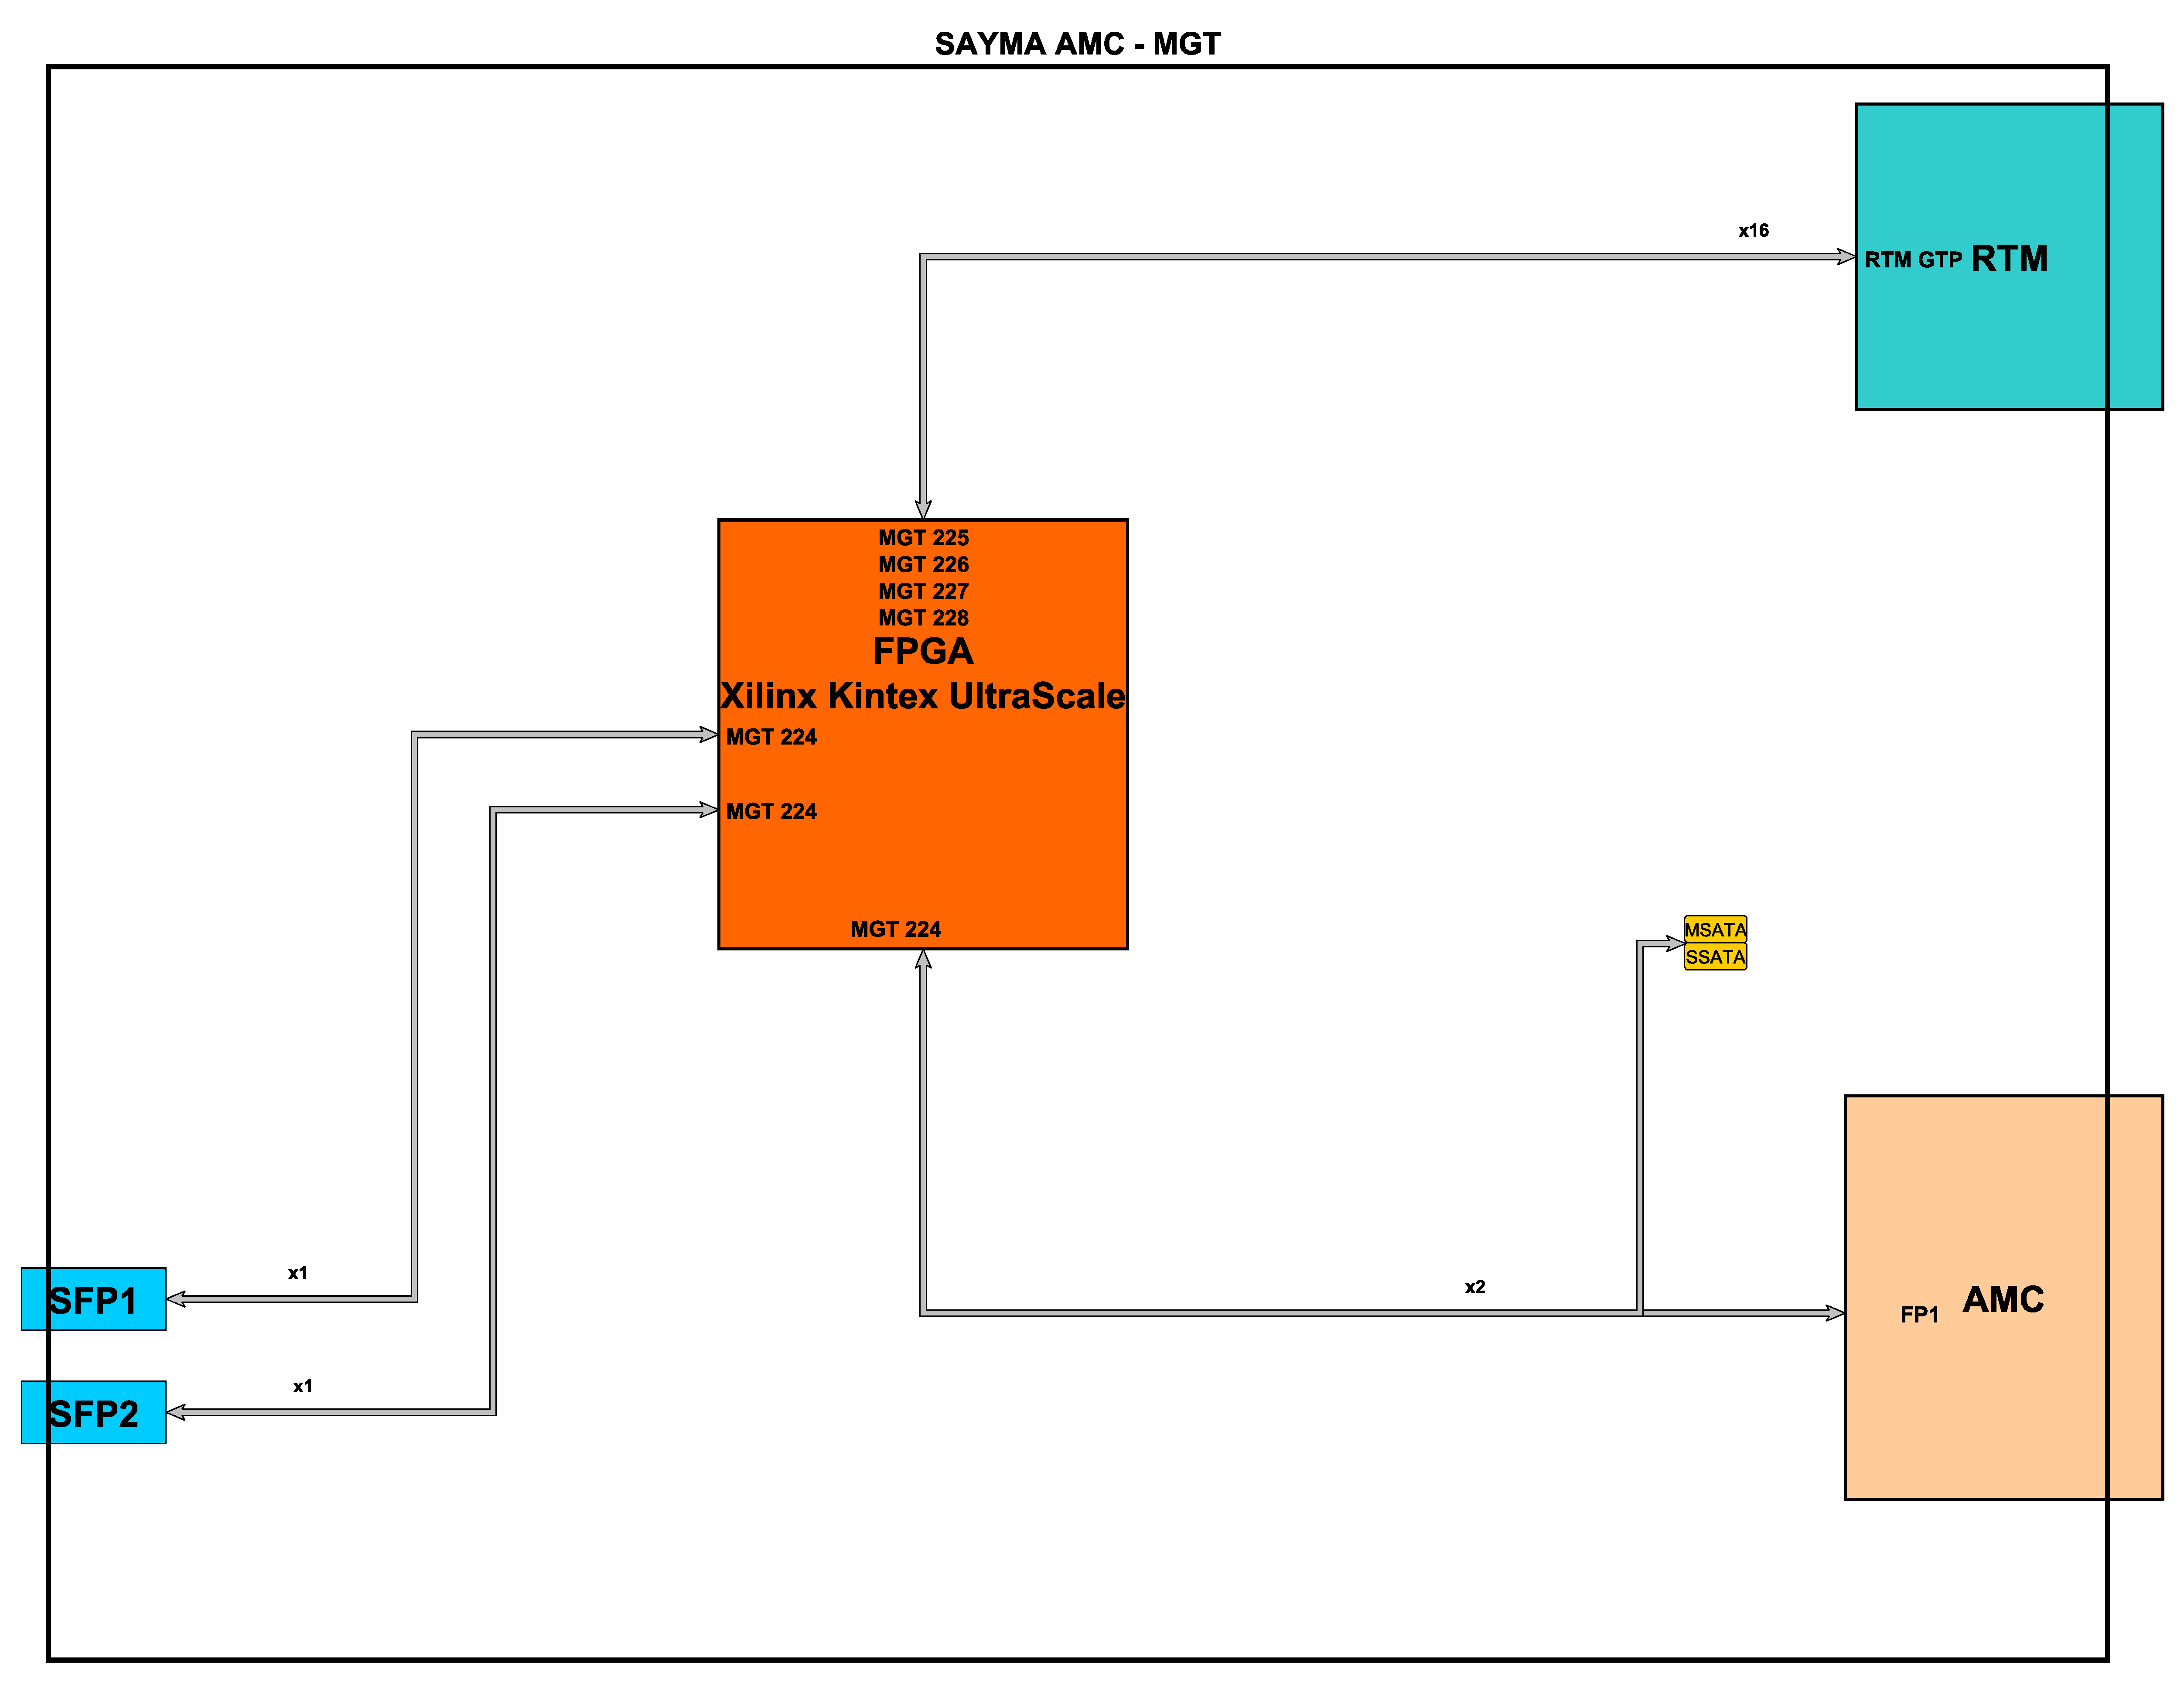
\includegraphics[scale=0.2]{img/sch_mgt.eps}\\
		\caption{MGT} \label{MGT}
	\end{figure}

	\begin{figure}[htbp!]
		\centering
		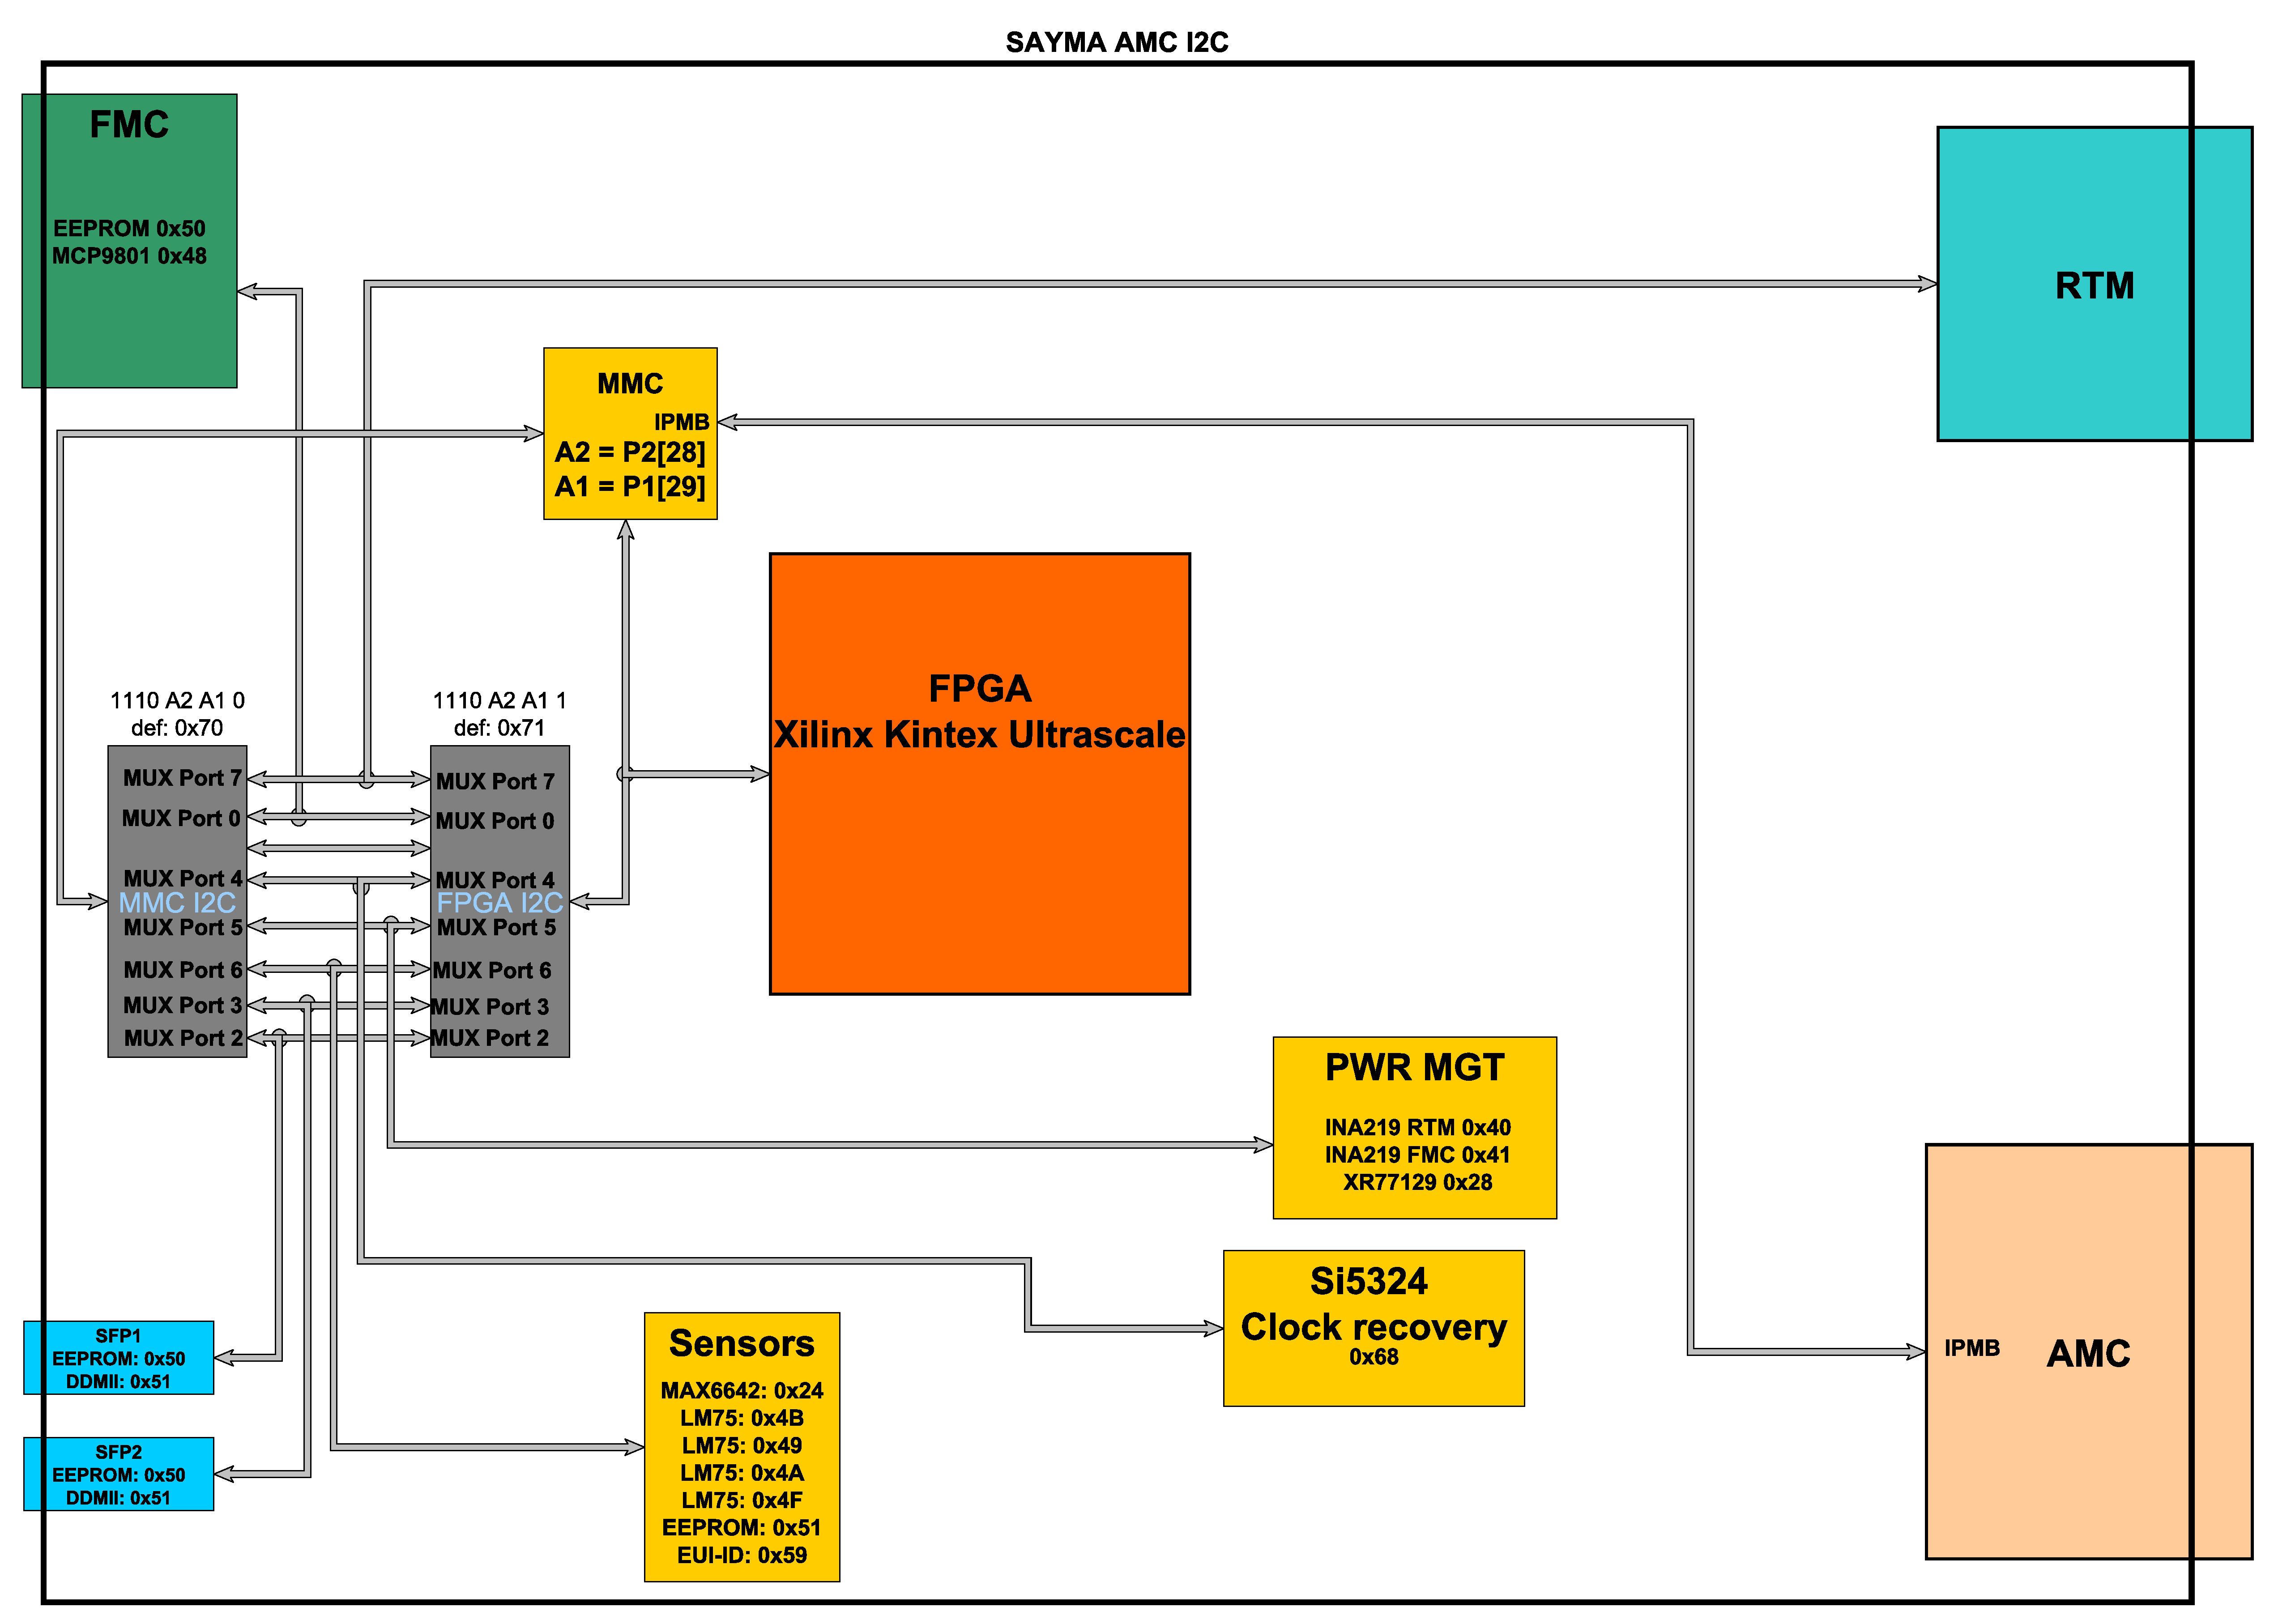
\includegraphics[scale=0.2]{img/i2c.eps}\\
		\caption{I2C} \label{I2C}
	\end{figure}


\clearpage

\section{Clocking}

This section describes how and where clock signals are routed.

	\begin{figure}[htbp!]
		\centering
		
\includegraphics[scale=0.2]{img/clk.eps}\\
		\caption{Clocks} \label{clocking}
	\end{figure}


\clearpage

\section{Front panel and headers}

		\begin{figure}[htbp!]
			\centering
			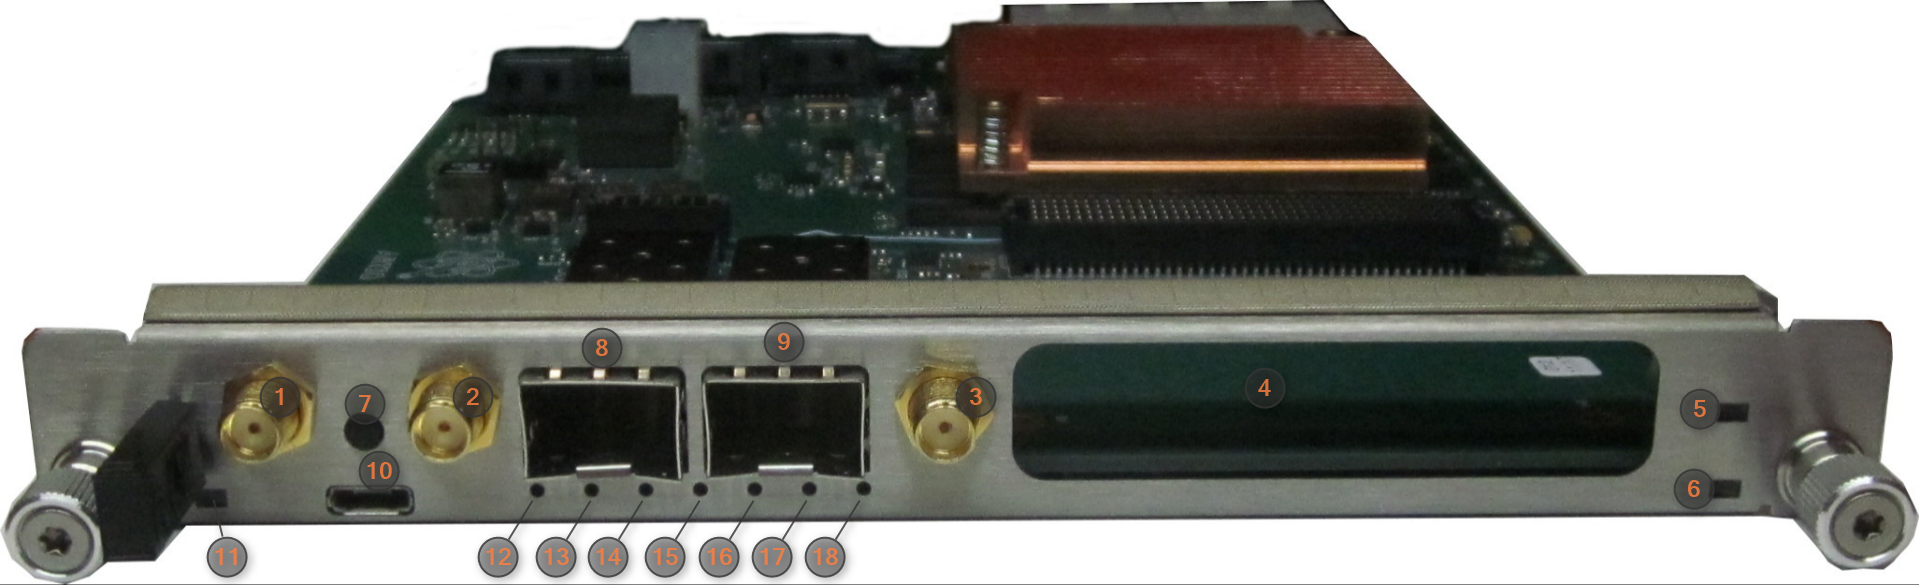
\includegraphics[width=14cm]{img/frontcallout.png}\\
			\caption{Front view}
		\end{figure}
		
		\begin{figure}[htbp!]
			\centering
			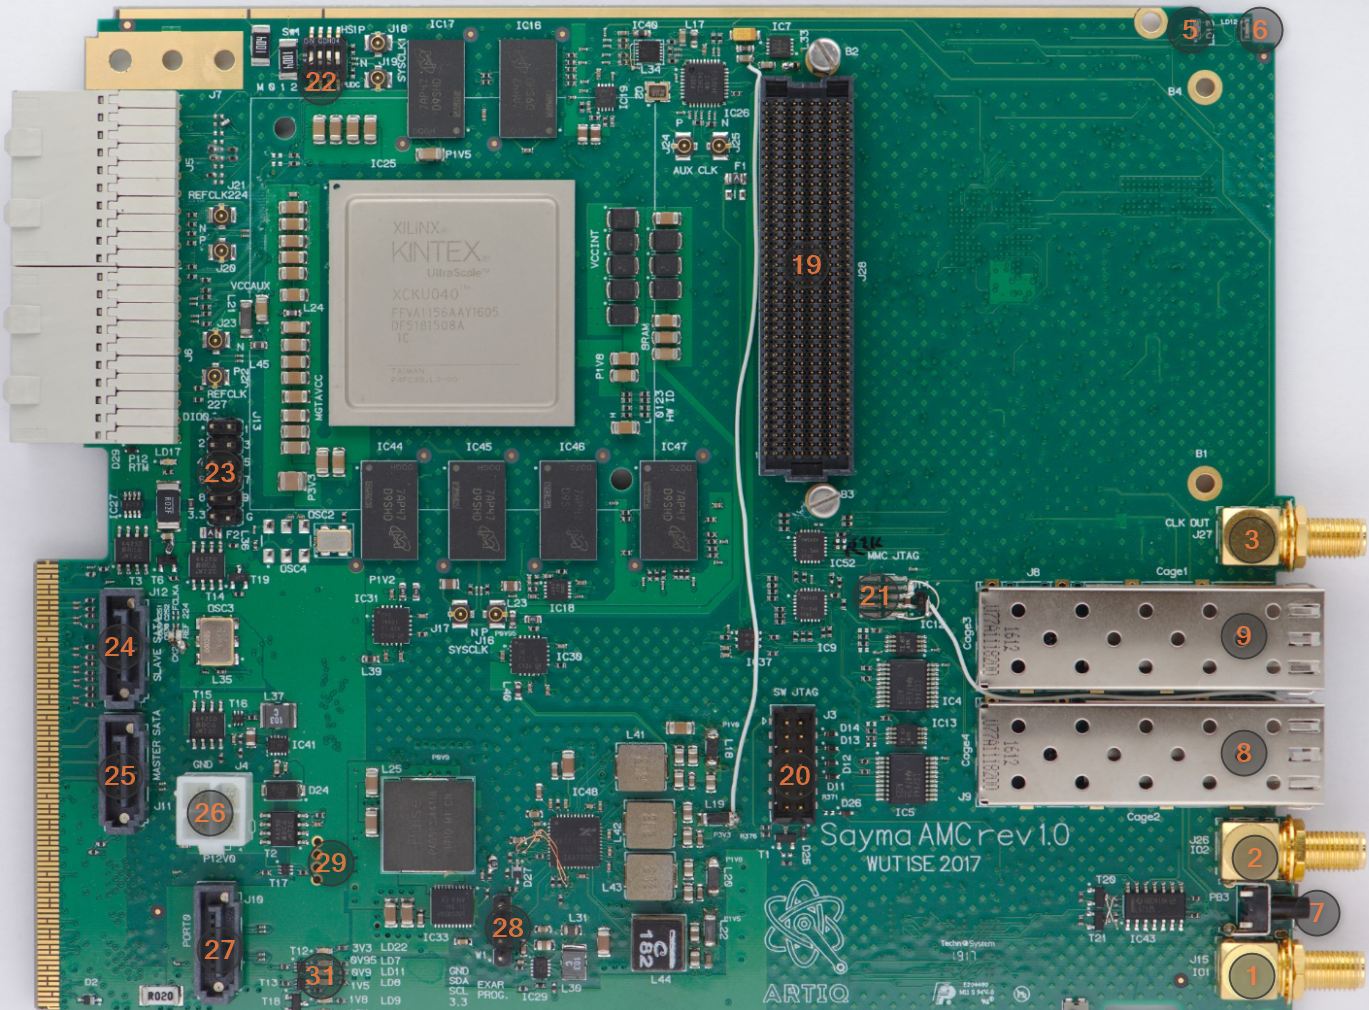
\includegraphics[width=14cm]{img/topcallout1.png}\\
			\caption{Front view}
		\end{figure}
\clearpage
		\begin{figure}[htbp!]
			\centering
			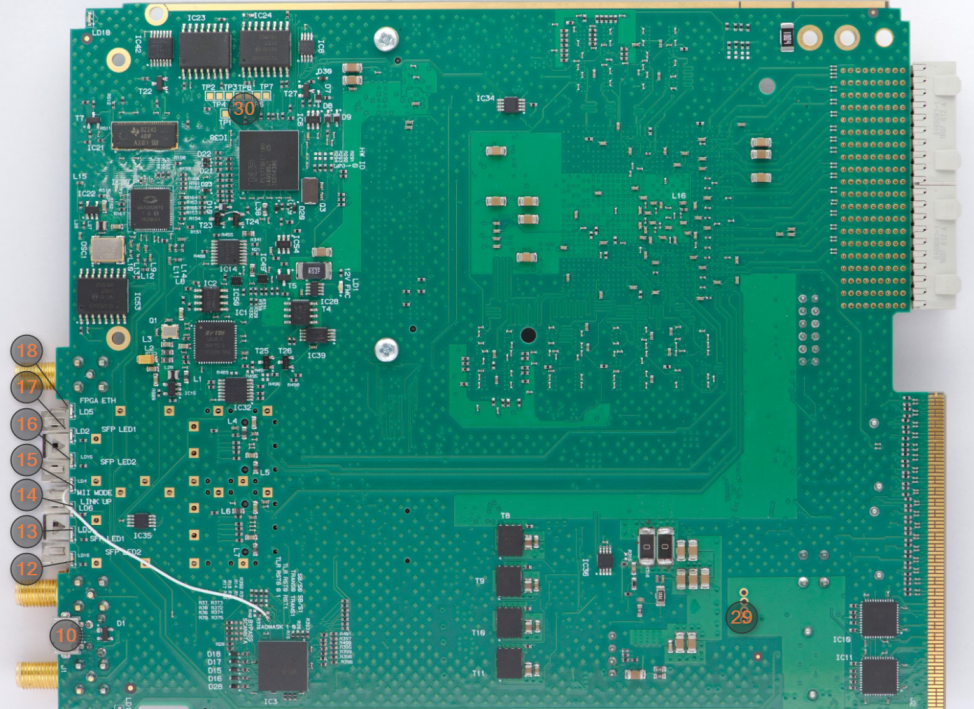
\includegraphics[width=14cm]{img/botcallout1.png}\\
			\caption{Front view}
		\end{figure}

\begin{longtable}{|c|c|c|} \hline
	\multicolumn{3}{|c|}{Call out table } \\ \hline	
	Call out & Designator & Description \\ \hline
	1 & J15 & IO1 \\ \hline
	2 & J26 & IO2 \\ \hline
	3 & J27 & CLK OUT \\ \hline
	4 & -- & FMC slot \\ \hline
%	5 & LD13 & Error\\ \hline
%	6 & LD18 & Hot swap \\ \hline
	7 & PB3 & reset? \\ \hline
	8 & cage2 & SFP Cage \\ \hline
	9 & cage1 & SFP Cage \\ \hline
	10 & J1 & Micro USB -->Serial \\ \hline
%	11& LD14 & operation successful  \\ \hline
%	12 & LD16 & SFP LED2 \\ \hline
%	13 & LD3 & SFP LED1 \\ \hline
%	14 & LD6 & LINK UP \\ \hline
%	15 & LD4 & MII MODE \\ \hline
%	16 & LD15 & SFP LED2  \\ \hline
%	17 & LD2 & SFP LED1 \\ \hline
%	18 & LD5 & FPGA ETH \\ \hline
	19 & J28 & FMC Header \\ \hline
	20 & J3 & SW JTAG \\ \hline
	21 & J14 & MMC JTAG \\ \hline
	22 & SW1 & FPGA MODE \\ \hline
	23 & J13 & Digital IOs \\ \hline
	24 & J12 & SLAVE SATA \\ \hline
	25 & J11 & MASTER SATA \\ \hline
	26 & J4 & Power In \\ \hline
	27 & J10 & Port 0 \\ \hline
	28 & W1 & EXAR I2C header \\ \hline
	29 & -- & P12V0 \\ \hline
	30 & -- &  Test points \\ \hline
\end{longtable}

\begin{longtable}{|c|c|c|c|c|c|c|} \hline
		\multicolumn{7}{|c|}{LED table }\\ \hline
	Call out & Designator & Description&  Colour &nominal state& IC &Failure\\ \hline
	5 & LD13 & Error &Red & off &MMC & on \\ \hline
	6 & LD4 & Hot Swap & Blue & on&  MMC &  off\\ \hline
	6 & LD21 & FPGA config done & Green & on& FPGA &off \\ \hline 
	11 & LD14 & Operation succesful& Green & on& MMC &off\\ \hline
	12 & LD3 & SFP2 LED2 & Red &on& FPGA & off\\ \hline
	13 & LD6 & SFP2 LED1 & Green &on & FPGA&off \\ \hline
	14 & LD20 & LINK UP &  Green &on & MAX24287&off \\ \hline
	15 & LD18 & MII MODE & Green & on& MMC&off \\ \hline
	16 & LD2 & SFP1 LED2 & Red & on& FPGA &off\\ \hline
	17& LD5 & SFP1 LED1 & Green &on & FPGA& off\\ \hline
	18 & LD19 & FPGA ETH & Green &on & MMC &off\\ \hline
	30 & LD22 & 3V3 & Green & on & Power & off \\ \hline
	30 & LD7 & 0V95 & Green & on & Power & off \\ \hline 
	30 & LD11 & 0V9 & Green & on & Power & off \\ \hline 
	30 & LD8 & 1V5 & Green & on & Power & off \\ \hline 
	30 & LD9 & 1V8 & Green & on & Power & off \\ \hline 
	30 & LD10 & 12V & Green & on & Power & off \\ \hline  
\end{longtable}

\subsection{Headers pinout}

		\begin{figure}[htbp!]
			\centering
			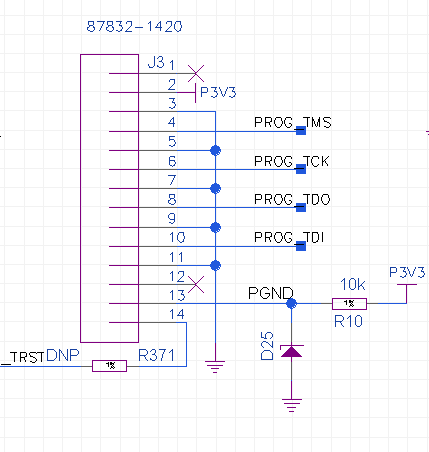
\includegraphics[width=9cm]{img/jtag1.png}\\
			\caption{JTAG - Call out 20}
		\end{figure}

		\begin{figure}[htbp!]
			\centering
			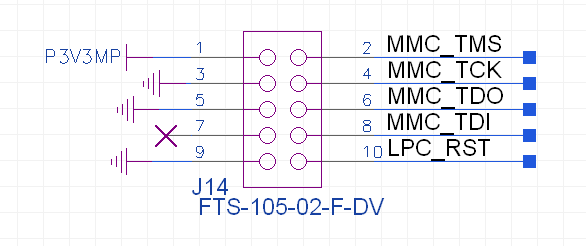
\includegraphics[width=9cm]{img/jtaglpc.png}\\
			\caption{JTAG - Call out  21}
		\end{figure}
		
		\begin{figure}[htbp!]
			\centering
			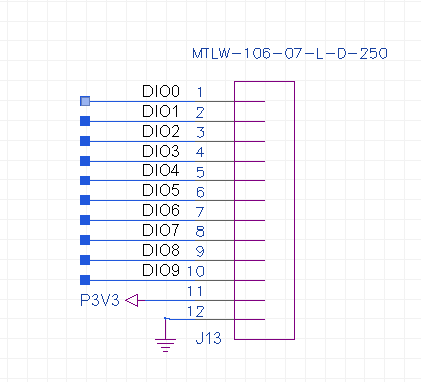
\includegraphics[width=9cm]{img/gpio.png}\\
			\caption{DIO - Call out 23}
		\end{figure}

\clearpage


\begin{longtable}{|c|c|c|} \hline
		\multicolumn{3}{|c|}{Tespoints table - Call out 30}\\ \hline
	TPx & Sig Name & LPC pin \\ \hline
	TP1 & MII1\_col & C13 \\ \hline
	TP2 & SDCLK & J10 \\ \hline
	TP3 & SDCMD & K14 \\ \hline
	TP4 & SDPWR & K11 \\ \hline
	TP5 & SDDAT0 & L14 \\ \hline
	TP6 & SDDAT1 & M12 \\ \hline
	TP7 & SDDAT2 & N14 \\ \hline
	TP8 & SDDAT3 & M11 \\ \hline
	
\end{longtable}	


\subsection{Location ICs}

		\begin{figure}[htbp!]
			\centering
			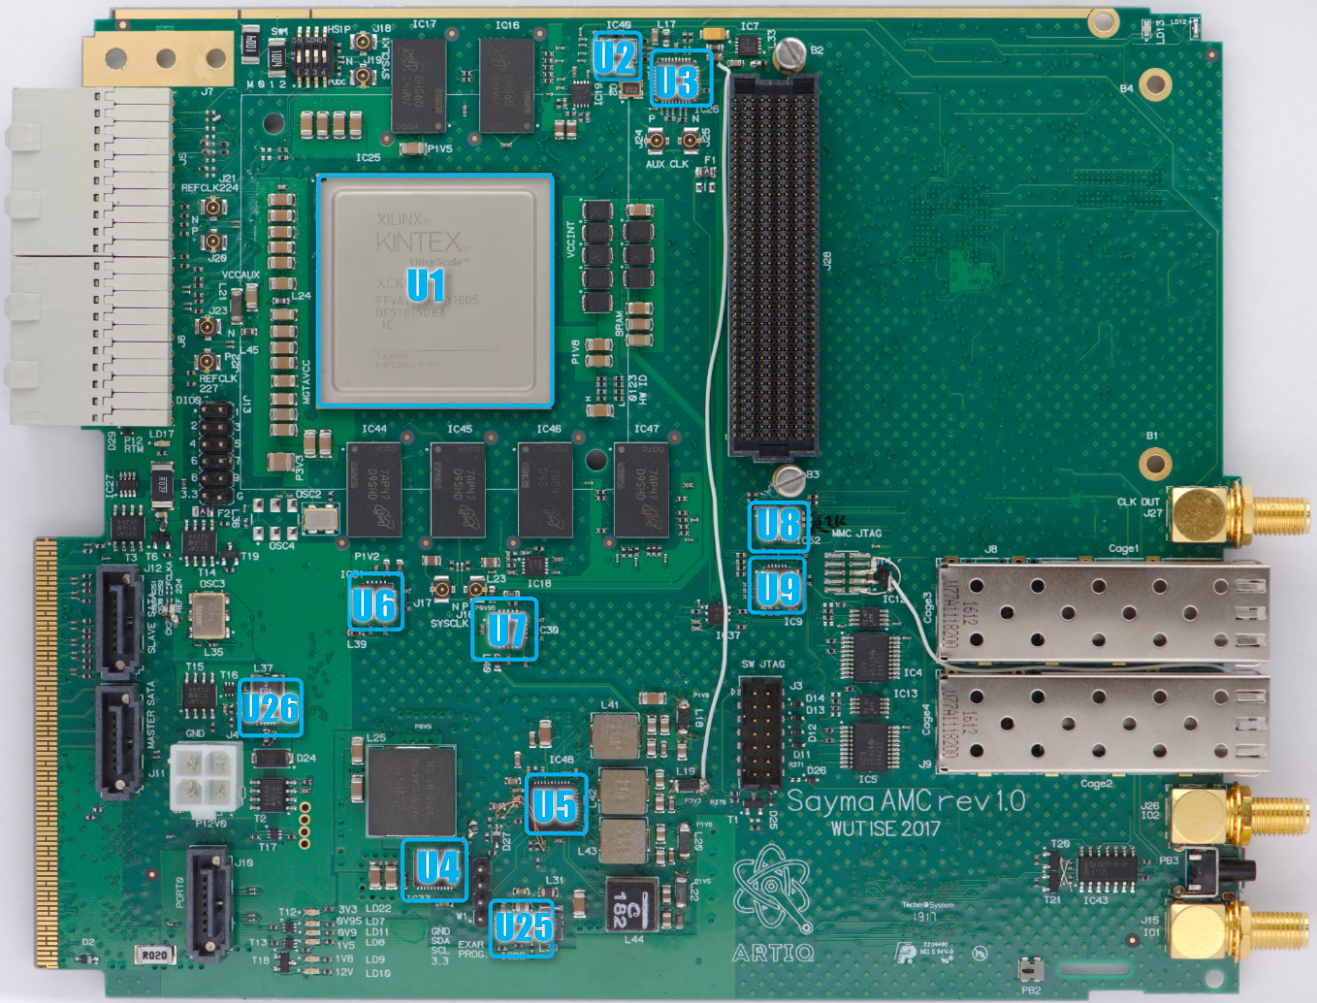
\includegraphics[width=14cm]{img/TU1.png}\\
			\caption{Top}
		\end{figure}
		\begin{figure}[htbp!]
			\centering
			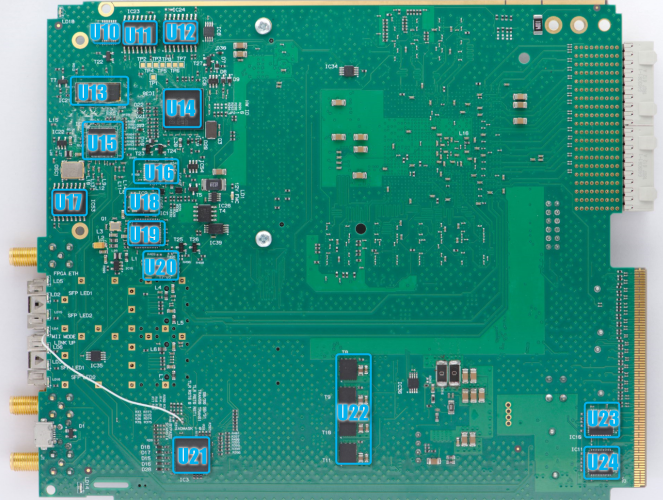
\includegraphics[width=14cm]{img/BU1.png}\\
			\caption{Bot}
		\end{figure}
\clearpage

\begin{longtable}{|c|c|c|} \hline
		\multicolumn{3}{|c|}{ICs Location}\\ \hline	
	Ux & IC & Description \\ \hline
	U1 & Kintex& FPGA \\ \hline
	U2 & LTC 6957&Low Phase Noise Buffer \\ \hline
	U4 & TPS53353  & P0V9\\ \hline
	U5 & XR77129 & EXAR\\ \hline
	U6 & TPS 74401  & P1V2\\ \hline
	U7 &  TPS 74401 & P0V95 \\ \hline
	U3 & SI5324C& Clock recovery \\ \hline
	U8 & TCA9548 &I2C switch - MMC\\ \hline
	U9 & TCA9548 &I2C switch - FPGA\\ \hline
	U10 & 74HC4066PW & Analog switch - Flash update\\ \hline
	U11 & N25Q256A13ESF40 & NOR Flash\\ \hline
	U12 & N25Q256A13ESF40 & NOR Flash\\ \hline
	U13 & SN74CB3Q32245ZKE  & Digital Bus switch - RGMI/MII\\ \hline
	U14 & LPC1776FET180  & MMC\\ \hline
	U15 & MAX24287ETK+ &ETH switch\\ \hline
	U16 & AN74CBT3257PW  & USB console switch\\ \hline
	U17 & N25Q256A13ESF40 & NOR Flash - MMC\\ \hline
	U18 & M93C46  & EEPROM\\ \hline
	U19 & F4232H-56Q & USB-UART Bridge \\ \hline
	U20 & 74HC4066PW & USB-UART Switch\\ \hline
	U21 & SCANSTA112SM & SCANSTA JTAG Switch\\ \hline
	U22 & FDMS7608S &EXAR Transistors \\ \hline
	U23 & SN65MLVD040RGZT &LVDS transceiver\\ \hline
	U24 & SN65MLVD040RGZT &LVDS transceiver \\ \hline
	U25 & TPS62175  & P5V0 \\ \hline
	U26 & TPS62175 & P3V3 \\ \hline
\end{longtable}


\subsection{SW1}

\begin{longtable}{|c|c|c|c|} \hline
			\multicolumn{4}{|c|}{SW1 table}\\ \hline
	M0 & M1 & M2 & Description \\ \hline
	0 & 0 & 0 & Master Serial Mode \\ \hline
	0 & 0 & 1 & Master Parallel Up \\ \hline
	0 & 1 & 1 & Master Parallel Down \\ \hline
	1 & 0 & 1 & Peripheral mode \\ \hline
	1 & 1 & 1 & Slave Serial mode \\ \hline
	
\end{longtable}	

\clearpage

\section{FMC}



\begin{itemize}
	\item VADJ: 1V8 @ 1A
	\item FPGA Banks: 47HP and 48HP
\end{itemize}


The connector is compliant with ANSI/VITA 57.1 FMC-LPC Standard.\\

%---------------------------------------------------------FMC1
\begin{footnotesize}
	\begin{longtable}{|p{7cm}|p{1cm}|p{5cm}|}
		\hline
		\multicolumn{3}{|c|}{\multirow{2}{*}{\textbf{\large{FMC1}}}}\\
		\multicolumn{3}{|c|}{} \\ \hline 
		FPGA signal	&	FPGA ball	&	Signal on the board	\\ \hline
		IO\_L12P\_T1U\_N10\_GC\_47	&	AA24	&	FMC1\_CLK0\_M2C\_P	\\ \hline
		IO\_L12N\_T1U\_N11\_GC\_47	&	AA25	&	FMC1\_CLK0\_M2C\_N	\\ \hline
		IO\_L11P\_T1U\_N8\_GC\_47	&	Y23	&	FMC1\_CLK1\_M2C\_P	\\ \hline
		IO\_L11N\_T1U\_N9\_GC\_47	&	AA23	&	FMC1\_CLK1\_M2C\_N	\\ \hline
		IO\_L12P\_T1U\_N10\_GC\_48	&	AC31	&	FMC1\_GBTCLK0\_M2C\_P	\\ \hline
		IO\_L12N\_T1U\_N11\_GC\_48	&	AC32	&	FMC1\_GBTCLK0\_M2C\_N	\\ \hline
		IO\_L1P\_T0L\_N0\_DBC\_48	&	AE27	&	FMC1\_DP0\_M2C\_P	\\ \hline
		IO\_L1N\_T0L\_N1\_DBC\_48	&	AF27	&	FMC1\_DP0\_M2C\_N	\\ \hline
		IO\_L2P\_T0L\_N2\_48	&	AE28	&	FMC1\_DP0\_C2M\_P	\\ \hline
		IO\_L2N\_T0L\_N3\_48	&	AF28	&	FMC1\_DP0\_C2M\_N	\\ \hline
		IO\_L13P\_T2L\_N0\_GC\_QBC\_48	&	AA32	&	FMC1\_LA00\_CC\_P	\\ \hline
		IO\_L13N\_T2L\_N1\_GC\_QBC\_48	&	AB32	&	FMC1\_LA00\_CC\_N	\\ \hline
		IO\_L14P\_T2L\_N2\_GC\_48	&	AB30	&	FMC1\_LA01\_CC\_P	\\ \hline
		IO\_L14N\_T2L\_N3\_GC\_48	&	AB31	&	FMC1\_LA01\_CC\_N	\\ \hline
		IO\_L8P\_T1L\_N2\_AD5P\_48	&	AF33	&	FMC1\_LA02\_P	\\ \hline
		IO\_L8N\_T1L\_N3\_AD5N\_48	&	AG34	&	FMC1\_LA02\_N	\\ \hline
		IO\_L21P\_T3L\_N4\_AD8P\_48	&	V33	&	FMC1\_LA03\_P	\\ \hline
		IO\_L21N\_T3L\_N5\_AD8N\_48	&	W34	&	FMC1\_LA03\_N	\\ \hline
		IO\_L7P\_T1L\_N0\_QBC\_AD13P\_48	&	AG31	&	FMC1\_LA04\_P	\\ \hline
		IO\_L7N\_T1L\_N1\_QBC\_AD13N\_48	&	AG32	&	FMC1\_LA04\_N	\\ \hline
		IO\_L10P\_T1U\_N6\_QBC\_AD4P\_48	&	AE33	&	FMC1\_LA05\_P	\\ \hline
		IO\_L10N\_T1U\_N7\_QBC\_AD4N\_48	&	AF34	&	FMC1\_LA05\_N	\\ \hline
		IO\_L15P\_T2L\_N4\_AD11P\_48	&	AC34	&	FMC1\_LA06\_P	\\ \hline
		IO\_L15N\_T2L\_N5\_AD11N\_48	&	AD34	&	FMC1\_LA06\_N	\\ \hline
		IO\_L18P\_T2U\_N10\_AD2P\_48	&	AC33	&	FMC1\_LA07\_P	\\ \hline
		IO\_L18N\_T2U\_N11\_AD2N\_48	&	AD33	&	FMC1\_LA07\_N	\\ \hline
		IO\_L11P\_T1U\_N8\_GC\_48	&	AD30	&	FMC1\_LA08\_P	\\ \hline
		IO\_L11N\_T1U\_N9\_GC\_48	&	AD31	&	FMC1\_LA08\_N	\\ \hline
		IO\_L9P\_T1L\_N4\_AD12P\_48	&	AE32	&	FMC1\_LA09\_P	\\ \hline
		IO\_L9N\_T1L\_N5\_AD12N\_48	&	AF32	&	FMC1\_LA09\_N	\\ \hline
		IO\_L17P\_T2U\_N8\_AD10P\_48	&	AA34	&	FMC1\_LA10\_P	\\ \hline
		IO\_L17N\_T2U\_N9\_AD10N\_48	&	AB34	&	FMC1\_LA10\_N	\\ \hline
		IO\_L16P\_T2U\_N6\_QBC\_AD3P\_48	&	AA29	&	FMC1\_LA11\_P	\\ \hline
		IO\_L16N\_T2U\_N7\_QBC\_AD3N\_48	&	AB29	&	FMC1\_LA11\_N	\\ \hline
		IO\_L24P\_T3U\_N10\_48	&	V31	&	FMC1\_LA12\_P	\\ \hline
		IO\_L24N\_T3U\_N11\_48	&	W31	&	FMC1\_LA12\_N	\\ \hline
		IO\_L19P\_T3L\_N0\_DBC\_AD9P\_48	&	W33	&	FMC1\_LA13\_P	\\ \hline
		IO\_L19N\_T3L\_N1\_DBC\_AD9N\_48	&	Y33	&	FMC1\_LA13\_N	\\ \hline
		IO\_L23P\_T3U\_N8\_48	&	U34	&	FMC1\_LA14\_P	\\ \hline
		IO\_L23N\_T3U\_N9\_48	&	V34	&	FMC1\_LA14\_N	\\ \hline
		IO\_L22P\_T3U\_N6\_DBC\_AD0P\_48	&	Y31	&	FMC1\_LA15\_P	\\ \hline
		IO\_L22N\_T3U\_N7\_DBC\_AD0N\_48	&	Y32	&	FMC1\_LA15\_N	\\ \hline
		IO\_L20P\_T3L\_N2\_AD1P\_48	&	W30	&	FMC1\_LA16\_P	\\ \hline
		IO\_L20N\_T3L\_N3\_AD1N\_48	&	Y30	&	FMC1\_LA16\_N	\\ \hline
		IO\_L13P\_T2L\_N0\_GC\_QBC\_47	&	W23	&	FMC1\_LA17\_CC\_P	\\ \hline
		IO\_L13N\_T2L\_N1\_GC\_QBC\_47	&	W24	&	FMC1\_LA17\_CC\_N	\\ \hline
		IO\_L14P\_T2L\_N2\_GC\_47	&	W25	&	FMC1\_LA18\_CC\_P	\\ \hline
		IO\_L14N\_T2L\_N3\_GC\_47	&	Y25	&	FMC1\_LA18\_CC\_N	\\ \hline
		IO\_L16P\_T2U\_N6\_QBC\_AD3P\_47	&	V22	&	FMC1\_LA19\_P	\\ \hline
		IO\_L16N\_T2U\_N7\_QBC\_AD3N\_47	&	V23	&	FMC1\_LA19\_N	\\ \hline
		IO\_L17P\_T2U\_N8\_AD10P\_47	&	T22	&	FMC1\_LA20\_P	\\ \hline
		IO\_L17N\_T2U\_N9\_AD10N\_47	&	T23	&	FMC1\_LA20\_N	\\ \hline
		IO\_L18P\_T2U\_N10\_AD2P\_47	&	V21	&	FMC1\_LA21\_P	\\ \hline
		IO\_L18N\_T2U\_N11\_AD2N\_47	&	W21	&	FMC1\_LA21\_N	\\ \hline
		IO\_L15P\_T2L\_N4\_AD11P\_47	&	U21	&	FMC1\_LA22\_P	\\ \hline
		IO\_L15N\_T2L\_N5\_AD11N\_47	&	U22	&	FMC1\_LA22\_N	\\ \hline
		IO\_L10P\_T1U\_N6\_QBC\_AD4P\_47	&	AB21	&	FMC1\_LA23\_P	\\ \hline
		IO\_L10N\_T1U\_N7\_QBC\_AD4N\_47	&	AC21	&	FMC1\_LA23\_N	\\ \hline
		IO\_L8P\_T1L\_N2\_AD5P\_47	&	AC22	&	FMC1\_LA24\_P	\\ \hline
		IO\_L8N\_T1L\_N3\_AD5N\_47	&	AC23	&	FMC1\_LA24\_N	\\ \hline
		IO\_L9P\_T1L\_N4\_AD12P\_47	&	AA20	&	FMC1\_LA25\_P	\\ \hline
		IO\_L9N\_T1L\_N5\_AD12N\_47	&	AB20	&	FMC1\_LA25\_N	\\ \hline
		IO\_L7P\_T1L\_N0\_QBC\_AD13P\_47	&	AA22	&	FMC1\_LA26\_P	\\ \hline
		IO\_L7N\_T1L\_N1\_QBC\_AD13N\_47	&	AB22	&	FMC1\_LA26\_N	\\ \hline
		IO\_L6P\_T0U\_N10\_AD6P\_47	&	AB25	&	FMC1\_LA27\_P	\\ \hline
		IO\_L6N\_T0U\_N11\_AD6N\_47	&	AB26	&	FMC1\_LA27\_N	\\ \hline
		IO\_L24P\_T3U\_N10\_47	&	V26	&	FMC1\_LA28\_P	\\ \hline
		IO\_L24N\_T3U\_N11\_47	&	W26	&	FMC1\_LA28\_N	\\ \hline
		IO\_L23P\_T3U\_N8\_47	&	V29	&	FMC1\_LA29\_P	\\ \hline
		IO\_L23N\_T3U\_N9\_47	&	W29	&	FMC1\_LA29\_N	\\ \hline
		IO\_L22P\_T3U\_N6\_DBC\_AD0P\_47	&	U26	&	FMC1\_LA30\_P	\\ \hline
		IO\_L22N\_T3U\_N7\_DBC\_AD0N\_47	&	U27	&	FMC1\_LA30\_N	\\ \hline
		IO\_L21P\_T3L\_N4\_AD8P\_47	&	W28	&	FMC1\_LA31\_P	\\ \hline
		IO\_L21N\_T3L\_N5\_AD8N\_47	&	Y28	&	FMC1\_LA31\_N	\\ \hline
		IO\_L20P\_T3L\_N2\_AD1P\_47	&	U24	&	FMC1\_LA32\_P	\\ \hline
		IO\_L20N\_T3L\_N3\_AD1N\_47	&	U25	&	FMC1\_LA32\_N	\\ \hline
		IO\_L19P\_T3L\_N0\_DBC\_AD9P\_47	&	V27	&	FMC1\_LA33\_P	\\ \hline
		IO\_L19N\_T3L\_N1\_DBC\_AD9N\_47	&	V28	&	FMC1\_LA33\_N	\\ \hline
		VREF\_48	&	AA30	&	FMC1\_VREF\_A\_M2C	\\ \hline
		VREF\_47	&	V24	&	FMC1\_VREF\_A\_M2C	\\ \hline
		
	\end{longtable}
\end{footnotesize}
\clearpage

\section{USB-UART}
\subsection{UART Switch}

UART from FPGA is connected through Multiplexer (SN74CB3T3257PW). Selection between MMC and USB is preformes automaticly. When micro-USB is connected S siglnal is high and Multiplexer connects USB to FPGA.\\ 

\subsection{USB-UART bridge}

The USB-UART bridge (FT4232H) requires USB device drivers, vailable free from http://www.ftdichip.com,
which are used to make the FT4232H on the Mini Module appear as a four virtual COM ports (VCP). This
then allows the user to communicate with the USB interface via a standard PC serial emulation port
(TTY).\\ Another FTDI USB driver, the D2XX driver, can also be used with application software to directly
access the FT4232H on the Mini Module though a DLL. \\


\clearpage

\section{JTAG}

JTAG can be connected either from USB (FT4232H) or from IDC header. IDC header is permanenty connected to Scansta. \\
The USB-UART bridge can be enabled by setting high on ADBUS7.\\



	\begin{figure}[htbp!]
		\centering
		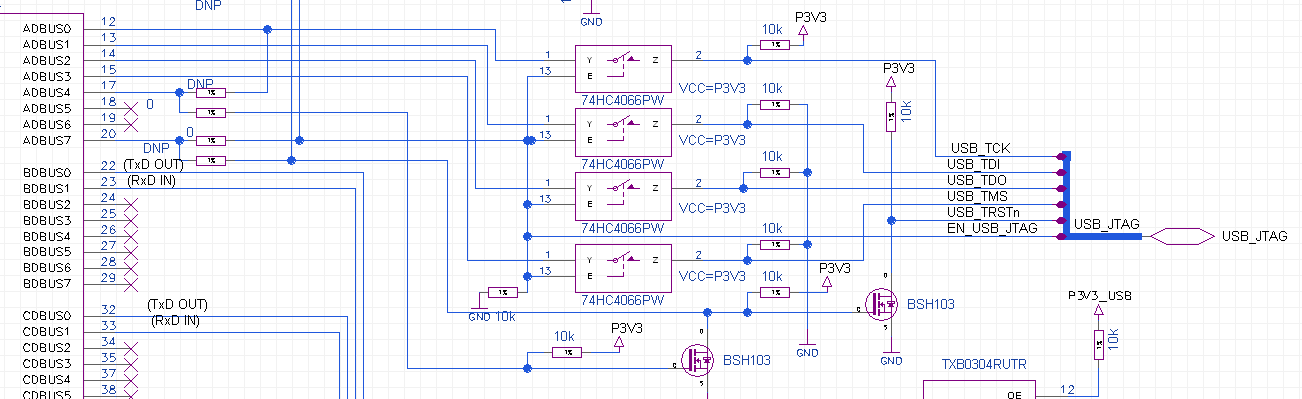
\includegraphics[scale=0.5]{img/jtag.png}\\
		\caption{USB-->JTAG} 
	\end{figure}
General block scheme of Scansta connections is shown below.\\
	
		\begin{figure}[htbp!]
			\centering
			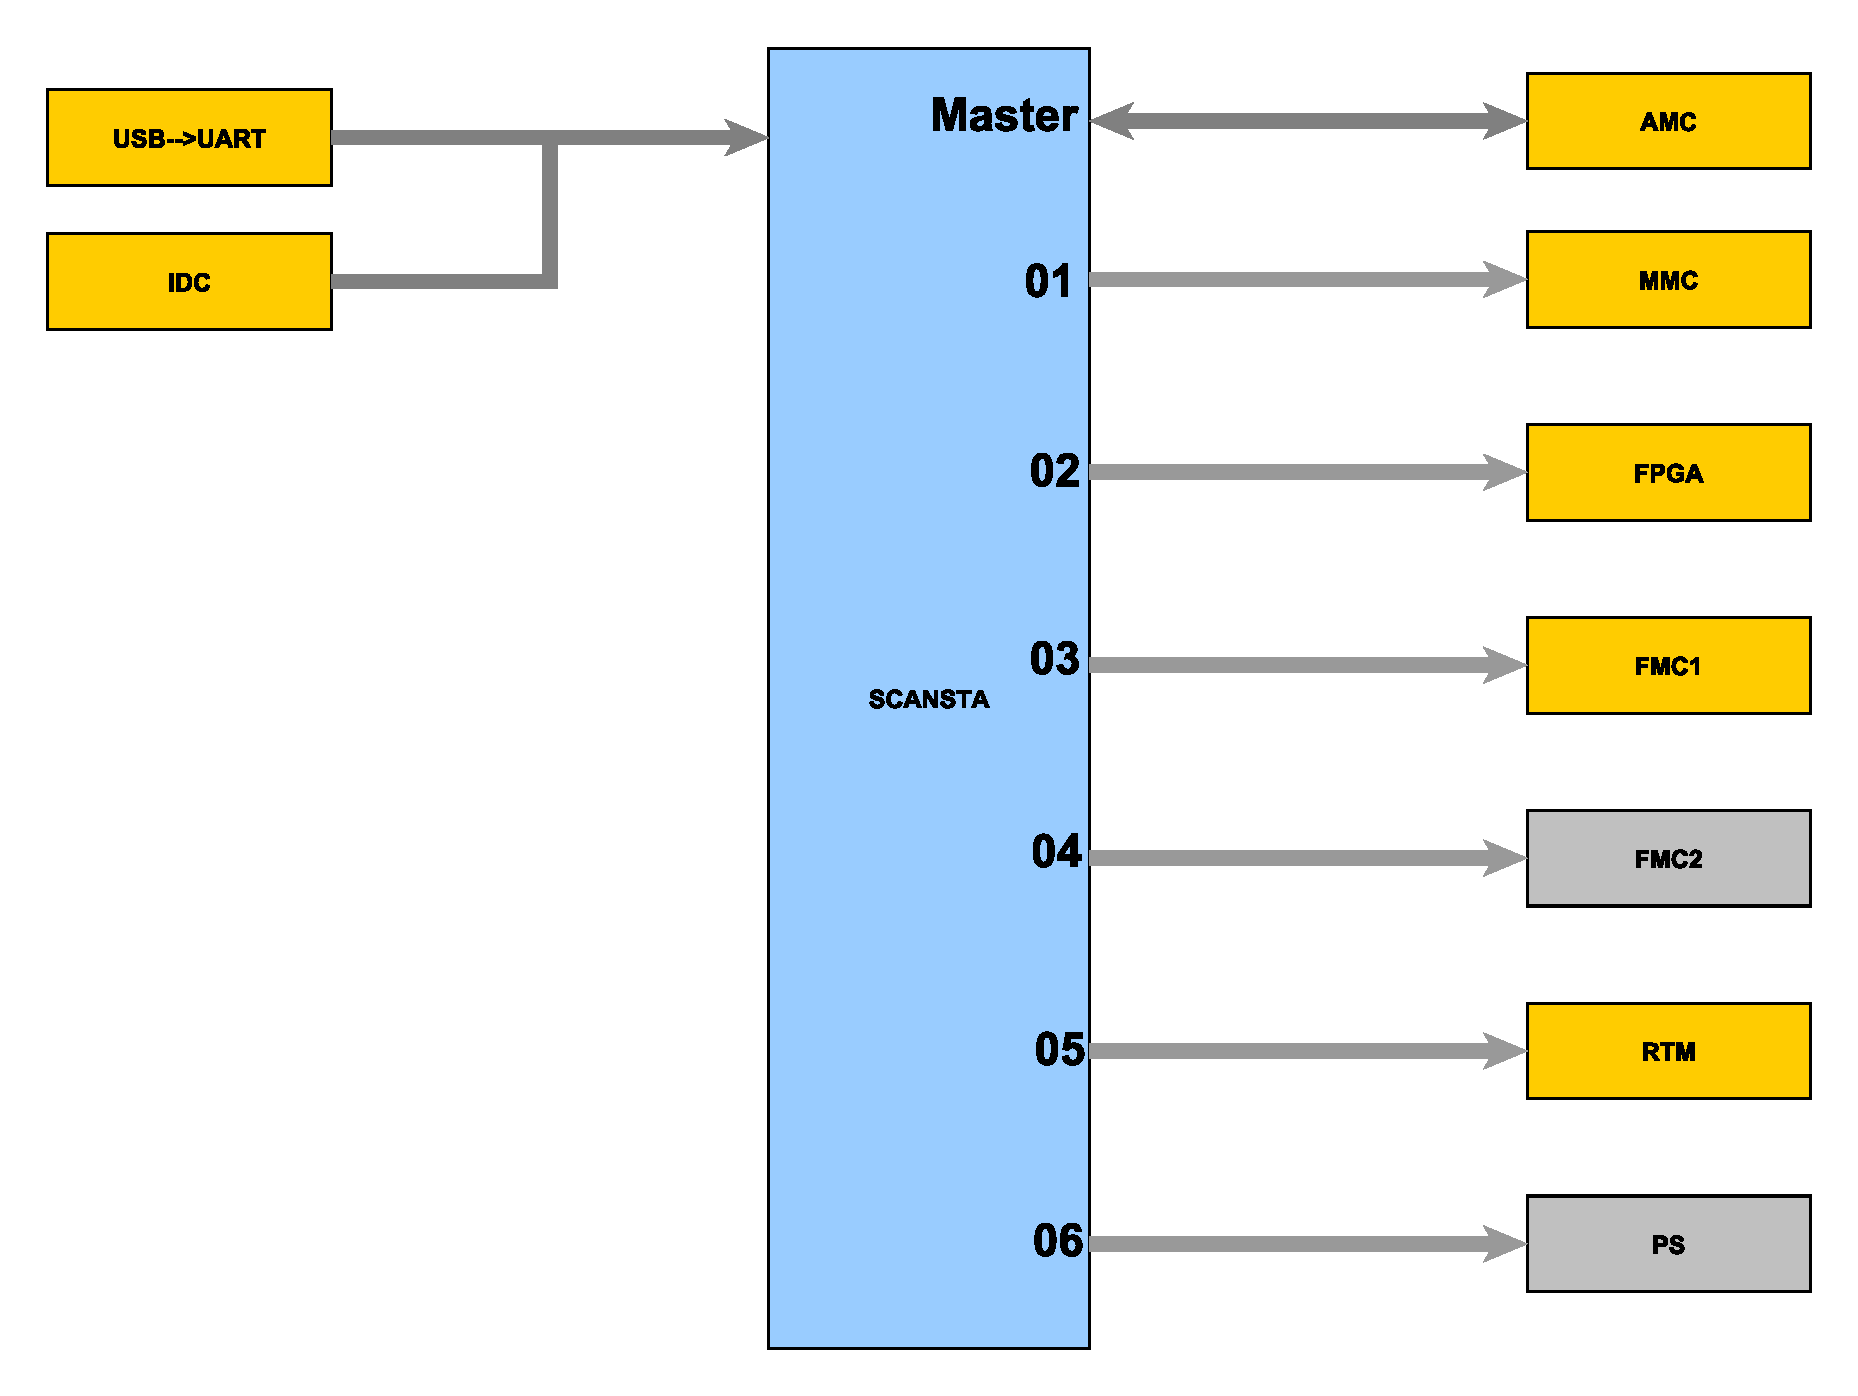
\includegraphics[scale=0.4]{img/scansta.eps}\\
			\caption{SCANSTA bloch scheme} 
		\end{figure}
		
	\textit{\textbf{Note:} The FMC2 and PS is not used.}\\
	
Scansta112 is 7-Port Multidrop JTAG Multiplexer. It is used to partition scan chains into managable sizes, or to isolate specific devices onto a separate chain. By default Scansta input signal is from IDC header. AMC JTAG is connected to Master Port on SCANSTA, so it can be used as Master or Slave module. The rest modules (MMC, FPGA, FMC, RTM) are tied to slave SCANSTA outputs. \\
Simplified instruction if using SCANSTA can be found under: \href{http://www.ti.com/lit/an/snla068c/snla068c.pdf}{http://www.ti.com/lit/an/snla068c/snla068c.pdf} 
In Sayma AMC, SCANSTA112 is used in Transparent Sticher Mode. In this mode, the IC can be configured via hardware to skip the addressing protocol needed, sothere is no need to run a SVF configuration file on IMPACT when programming the FPGA bitstream.

		\begin{figure}[htbp!]
			\centering
			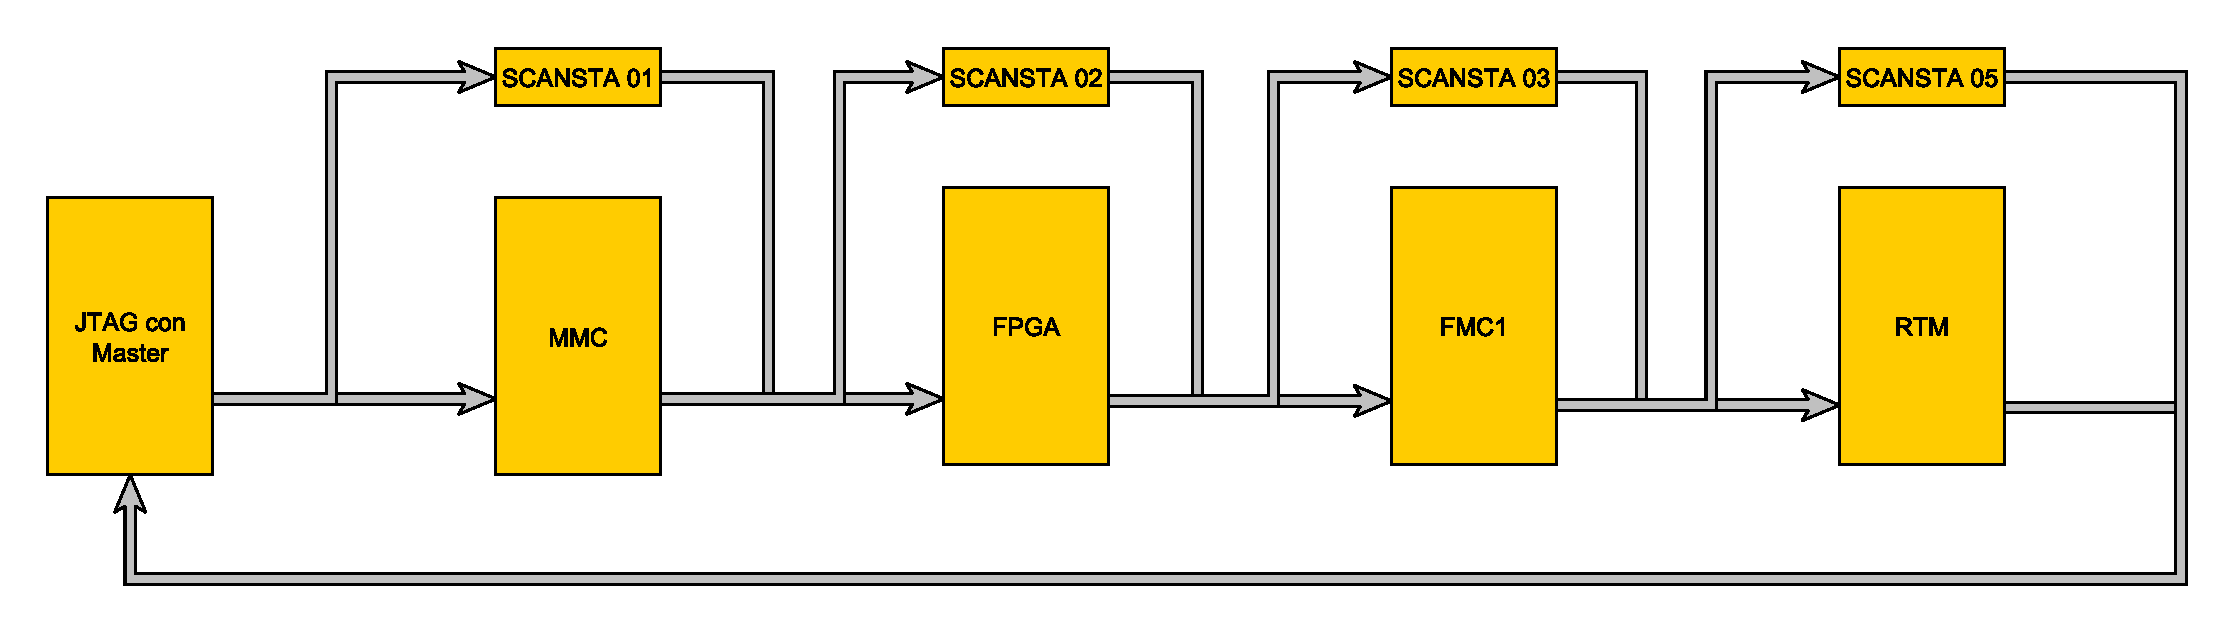
\includegraphics[scale=0.4]{img/jtagchain.eps}\\
			\caption{SCANSTA JTAG chain} 
		\end{figure}

\clearpage

\section{FPGA bootstrapping}


\noindent
\textbf{Xilinx User Guide:} \href{https://www.xilinx.com/support/documentation/user_guides/ug570-ultrascale-configuration.pdf}{https://www.xilinx.com/support/documentation/user\_guides/ug570-ultrascale-configuration.pdf}\\

To load FPGA .bit into flash Vivado in version minimum 16.4 is needed.\\
\textbf{Vivado WebPack:}\href{https://www.xilinx.com/support/download.html}{https://www.xilinx.com/support/download.html}

Alternatively Vivado Lab tools (previously Lab Tools) can be used.\\
\textbf{Vivado Lab Edition:}\href{https://www.xilinx.com/support/download.html}{https://www.xilinx.com/support/download.html}


\clearpage

\section{Power}
\subsection{Power supply}

\todo[inline]{TBD voltage noise}
The 12V power can be connected either from AMC connector or from Stand alone power supply connected to Molex Connector(39-28-1043).

	\begin{figure}[htbp!]
		\centering
		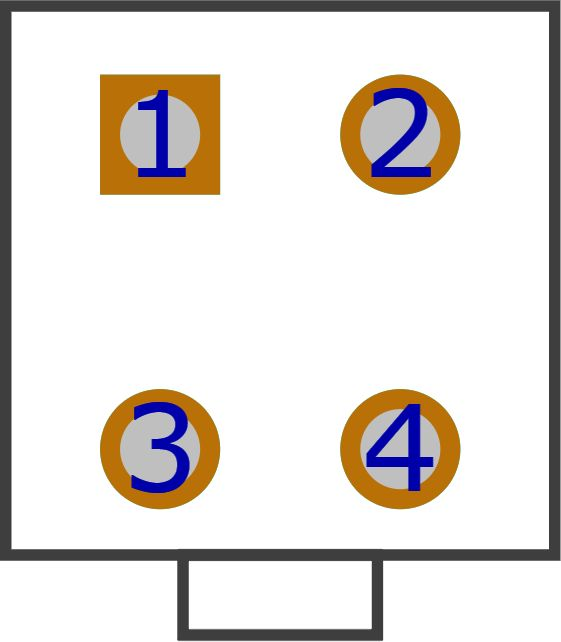
\includegraphics[scale=0.2]{img/molex.jpg}\\
		\caption{Power connector} 
	\end{figure}
\begin{center}
\begin{tabular}{|c|c|} \hline
	{\LARGE GND} & {\LARGE GND} \\ \hline
	{\LARGE +12} & {\LARGE +12} \\ \hline
\end{tabular}
\end{center}

Maximum board(AMC+RTM module) power consumption estimate to 3A @ 12V.\\

	\textit{\textbf{Note:} Please note that power consumption mostly depends from FPGA configuration. \\}

\begin{itemize}
 

\item Input voltage range: 10.8-13.2 [V]\\
\item The board needs active cooling. Approx. 20CFM in 20 C air.\\

\end{itemize}
\subsection{Power configuration} 

\subsubsection{Power map}


	\begin{figure}[htbp!]
		\centering
		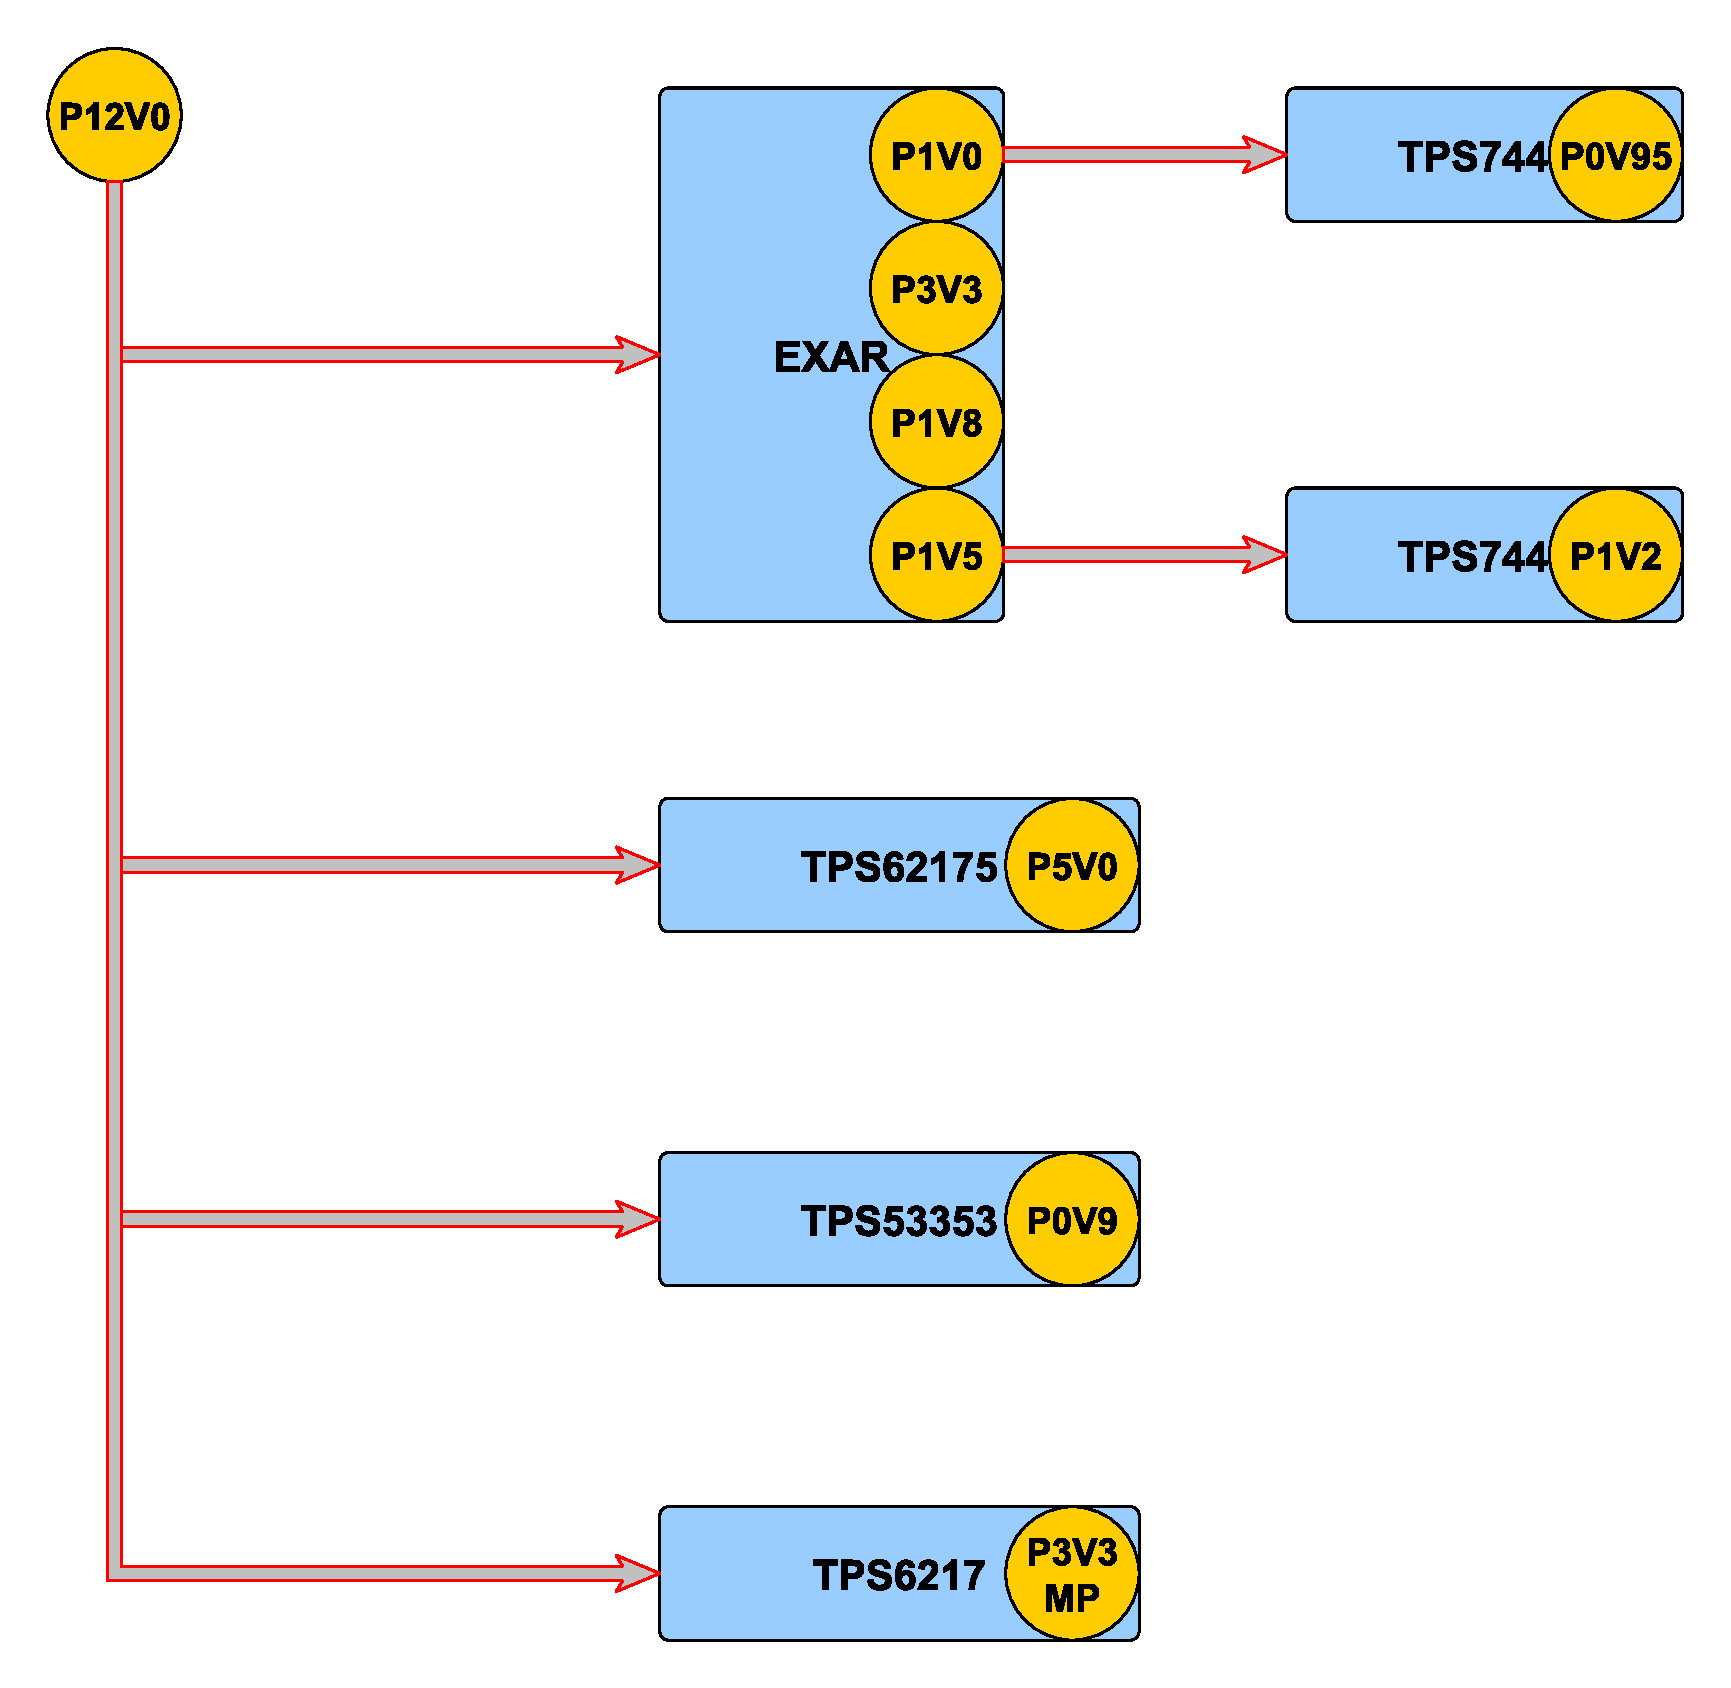
\includegraphics[scale=0.3]{img/pwr.eps}\\
		\caption{Power map} 
	\end{figure}
\clearpage	

\begin{longtable}{|c|c|c|} \hline
\multicolumn{3}{|c|}{voltages and currents}	\\ \hline
P0V9 & 0.9V & 10A \\ \hline
P0V95 & 0.95V & 31mA\\ \hline
P1V0 & 1.0V & 3A\\ \hline
P1V2 & 1.2V & 0.6A\\ \hline
P1V5 & 1.5V & 7.5A\\ \hline
P1V8 & 1.8V & 1.6A\\ \hline
P3V3 & 3.3 V & 2A\\ \hline
P3V3MP & 3.3V & 0.18A \\ \hline
P5V0 & 5.0V & 0.5A\\ \hline
\end{longtable}
	
\begin{longtable}{|c|c|c|} \hline
	\multicolumn{3}{|c|}{Maximum RTM voltages and currents}	\\ \hline
	P12V0 & 12V & 3A \\ \hline	
	P3V3MP\_RTM & 3.3V & 30mA \\ \hline
\end{longtable}
	
\subsubsection{Exar parameters}

Exar chip has 4 configurable outputs with configirable current limits. Channels 1, 3, 4 are power un on chip enable with 10ms delay. Channel 2 is power on 'EN\_PSU\_CH' signal. \\
%3V3 LDO is power on independently. \\

	\begin{figure}[htbp!]
		\centering
		\includegraphics[scale=0.6]{img/exar1.png}\\
		\caption{Exar configuration} 
	\end{figure}
	
	\begin{figure}[htbp!]
		\centering
		\includegraphics[scale=0.6]{img/exar2.png}\\
		\caption{Exar power on delays} 
	\end{figure}	
	
\clearpage	


\subsubsection{Exar configuration}
Exar chips are configured via I2C bus (MUX Port 5) or directly by connecting to W1 (call-out 28) header. For proper configuration \textbf{Exar Power Architect} in version \textbf{5.2-r1} is needed.
% Configuration files can be found at github in folder \href{https://github.com/m-labs/sinara/tree/master/EXAR\_config}{m-labs/sinara/Exar\_config}\\

\noindent
\textbf{Exar Power Archtect 5.2-r1:}
\href{https://www.exar.com/content/document.ashx?id=21632}{https://www.exar.com/content/document.ashx?id=21632}\\
\textbf{Configuration files:}
\href{https://github.com/m-labs/sinara/tree/master/EXAR\_config}{https://github.com/m-labs/sinara/tree/master/EXAR\_config}\\
\textbf{Datasheet:}\href{https://www.exar.com/ds/xr77129_1a_120514.pdf}{https://www.exar.com/ds/xr77129\_1a\_120514.pdf}\\
\textbf{Quick Start Guide:} \href{https://www.exar.com/files/powerxr/PA5-QSG_110_010614.pdf}{https://www.exar.com/files/powerxr/PA5-QSG\_110\_010614.pdf}\\


Actual voltages and current consumption, temperature can be found in Chip Dashboard. There is also oportunity to adjust settings.

	\begin{figure}[htbp!]
		\centering
		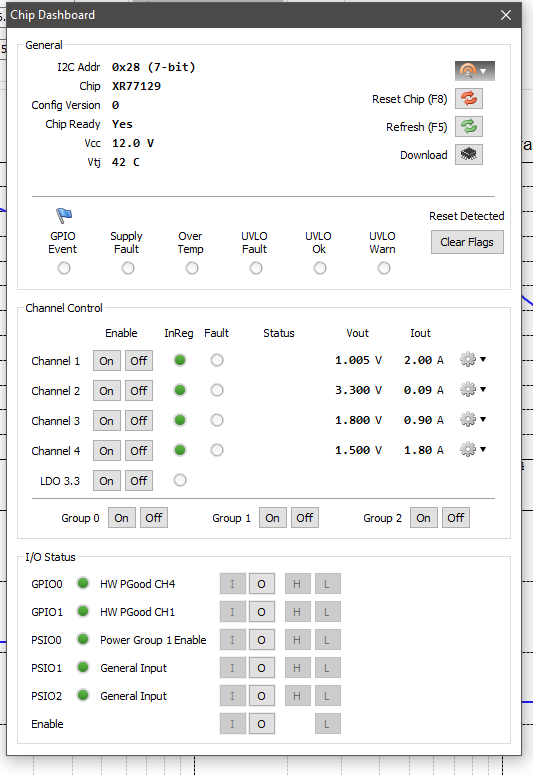
\includegraphics[scale=0.6]{img/exarprog.png}\\
		\caption{Chip Dashboard} 
	\end{figure}



\clearpage

\section{MMC}

\subsection{MMC steps during booting}

\begin{itemize}

\item configures CPU, UART
\item sets port directions
\item enables VCCINT PSU
\item enables P5V0 PSU (helper PSU)
\item enables Exar PSU. It boots from its own EEPROM
\item waits 200ms
\item configures SCANSTA chip in stitcher mode. If RTM is inserted, it enables its JTAG port
\item configures I2C switch base address
\item initializes default RTM power state to off
\item initializes Ethernet PHY chip in RGMII mode using pin strap.
\item waits 200ms
\item initializes I2C controller and chain (switch)
\item configures Si5324
\item checks if RTM is inserted, if yes, then enables its power, waits 200ms and initializes RTM power supply via I2C. It also configures Si5324 on RTM
\item runs task.\\

The task performs following functions:

\item blinks front panel LEDs alternately
\item checks if FPGA is configured. If not, it keeps Ethernet PHY in reset state. Once FPGA gets configured, it initializes the PHY.
\item checks if RTM is unplugged. If not, it switches the power off to make sure it is off during hotplug.
\end{itemize}

\subsection{Bootstraping}

The MMC can be upgraded by USB cable and NXP programmer(can be used other programmer but make sure that header shorts pins 3, 5, 9) using  \href{http://www.flashmagictool.com/}{Flashmagic} or any other software which can talk with NXP bootloader. The source code is written in C and can be found on github.\\ 
\textbf{Source code:} \href{https://github.com/m-labs/sinara/tree/master/SAYMA\_firmware}{https://github.com/m-labs/sinara/tree/master/SAYMA\_firmware}.\\
\textbf{pre-compiled binary:} \href{https://github.com/m-labs/mmc-firmware/releases}{https://github.com/m-labs/mmc-firmware/releases}\\

To compile binaries \href{https://www.nxp.com/products/processors-and-microcontrollers/arm-based-processors-and-mcus/lpc-cortex-m-mcus/lpc1100-cortex-m0-plus-m0/lpcxpresso-ide-v8.2.2:LPCXPRESSO?tab=Design_Tools_Tab}{LPCXpresso} is needed.

\subsection{Functionality}

\todo[inline]{needed?}

\subsection{Exar debugging}
 
In case of chip failure, i.g.overvoltage, overcurrent, etc., there is possibility  to check chip status via UART. In this case in UART console, Exar register readout can be done by typing 'P' character.\\

	\begin{figure}[htbp!]
		\centering
		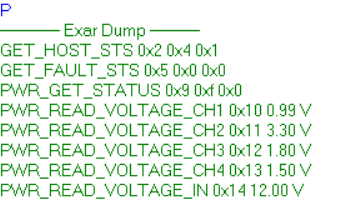
\includegraphics[scale=0.6]{img/exarreg.png}\\
		\caption{Exar register } 
	\end{figure}	
\clearpage
\subsection{PHY debugging}

In case of chip failure, there is possibility to check chip status via UART. In this case in UART console, Ethernet PHY content can be read by typing 'E' character

	\begin{figure}[htbp!]
		\centering
		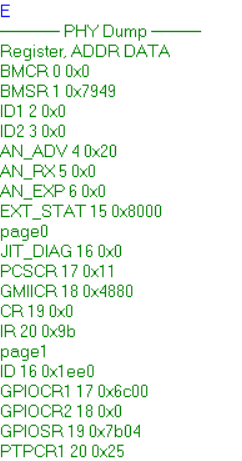
\includegraphics[scale=0.6]{img/phyreg.png}\\
		\caption{Ethernet PHY register } 
	\end{figure}

\subsection{RGMII Ethernet }

\todo[inline]{TBD. Not sure what should it contain.}

\subsection{OpenMMC}

\textbf{OpenMMC Project:}\href{https://github.com/lnls-dig/openMMC}{https://github.com/lnls-dig/openMMC}

\todo[inline]{TBD}

\clearpage

\section{Housekeeping Signals}
\subsection{sensors}
Temperature:\\
%\begin{itemize}
%	\item IC8 (0x4B) -NOR Flash
%	\item IC34 (0x49) -FPGA
%	\item IC35 (0x4A)-under SFPs
%	\item IC36 (0x4F)-power section
%	\item IC37 (0x24) -middle od the board
%\end{itemize}
\begin{longtable}{|c|c|c|c|c|}\hline
	No & Addr. & placement & Type & Accuracy \\ \hline
	IC8 & 0x4B & NOR Flash & LM75 & +/- 2 \\ \hline
	IC34 & 0x49 & FPGA & LM75 & +/- 2  \\ \hline
	IC35 & 0x4A & Under SFPs & LM75 & +/- 2  \\ \hline	
	IC36 & 0x4F & power section & LM75 & +/- 2  \\ \hline
	IC37 & 0x24 & middle of the board & MAX664A & +/- 1 \\ \hline
\end{longtable}

All temperature sensors are tied tohether to one I2C bus - I2C\_SENS. \\


Current:
%\begin{itemize}
%	\item IC27 (0x40)-RTM\_P12V0
%	\item IC28 (0x41)-FMC\_P12V0
%\end{itemize}
\begin{longtable}{|c|c|c|c|c|}\hline
		No & Addr. & placement & Type & Accuracy \\ \hline
		IC27 & 0x40 &RTM\_P12V0& INA219 & +/- 0.2\% \\ \hline
		IC28 & 0x41 &FMC\_P12V0& INA219 & +/- 0.2\% \\ \hline
\end{longtable}


All current sensors are tied tohether to one I2C bus - PM\_I2C. \\

\subsection{Safety interlocks}

\todo[inline]{TBD OVERTEMPn}

\clearpage


\section{Signal tables}
In this section the more important signals tables are presented. The total signal table is in Appendix section.\\
%---------------------------------------------------------SFP1
\begin{footnotesize}
	\begin{longtable}{|p{7cm}|p{1cm}|p{5cm}|}
	\hline
	\multicolumn{3}{|c|}{\multirow{2}{*}{\textbf{\large{SFP1}}}}\\
	\multicolumn{3}{|c|}{} \\ \hline
FPGA signal	&	FPGA ball	&	Signal on the board	\\ \hline 
MGTHTXN0\_224	&	AN3	&	SFP1TX\_N	\\ \hline
MGTHTXP0\_224	&	AN4	&	SFP1TX\_P	\\ \hline
MGTHRXN0\_224	&	AP1	&	SFP1RX\_N	\\ \hline
MGTHRXP0\_224	&	AP2	&	SFP1RX\_P	\\ \hline
IO\_L14N\_T2L\_N3\_GC\_64	&	AG9	&	SFP1\_LED1	\\ \hline
IO\_T2U\_N12\_64	&	AJ10	&	SFP1\_LED2	\\ \hline
IO\_L3P\_T0L\_N4\_AD15P\_64	&	AM11	&	SFP1\_LOS	\\ \hline
IO\_L2N\_T0L\_N3\_64	&	AP13	&	SFP1\_MOD\_DEF2	\\ \hline
IO\_L2P\_T0L\_N2\_64	&	AN13	&	SFP1\_MOD\_DEF1	\\ \hline
IO\_L3N\_T0L\_N5\_AD15N\_64	&	AN11	&	SFP1\_MOD\_DEF0	\\ \hline
IO\_T0U\_N12\_64	&	AK11	&	SFP1\_RATE\_SELECT	\\ \hline
IO\_L1P\_T0L\_N0\_DBC\_64	&	AP11	&	SFP1\_TX\_DISABLE	\\ \hline
IO\_L1N\_T0L\_N1\_DBC\_64	&	AP10	&	SFP1\_TX\_FAULT	\\ \hline
	

		
	\end{longtable}
\end{footnotesize}

%---------------------------------------------------------SFP2
\begin{footnotesize}
	\begin{longtable}{|p{7cm}|p{1cm}|p{5cm}|}
		\hline
		\multicolumn{3}{|c|}{\multirow{2}{*}{\textbf{\large{SFP2}}}}\\
		\multicolumn{3}{|c|}{} \\ \hline 
FPGA signal	&	FPGA ball	&	Signal on the board	\\ \hline
MGTHTXN1\_224	&	AM5	&	SFP2TX\_N	\\ \hline
MGTHTXP1\_224	&	AM6	&	SFP2TX\_P	\\ \hline
MGTHRXN1\_224	&	AM1	&	SFP2RX\_N	\\ \hline
MGTHRXP1\_224	&	AM2	&	SFP2RX\_P	\\ \hline
IO\_L8N\_T1L\_N3\_AD5N\_64	&	AJ13	&	SFP2\_LED1	\\ \hline
IO\_L7P\_T1L\_N0\_QBC\_AD13P\_64	&	AE13	&	SFP2\_LED2	\\ \hline
IO\_L7N\_T1L\_N1\_QBC\_AD13N\_64	&	AF13	&	SFP2\_LOS	\\ \hline
IO\_L5P\_T0U\_N8\_AD14P\_64	&	AK12	&	SFP2\_MOD\_DEF2	\\ \hline
IO\_L6N\_T0U\_N11\_AD6N\_64	&	AL13	&	SFP2\_MOD\_DEF1	\\ \hline
IO\_L6P\_T0U\_N10\_AD6P\_64	&	AK13	&	SFP2\_MOD\_DEF0	\\ \hline
IO\_L5N\_T0U\_N9\_AD14N\_64	&	AL12	&	SFP2\_RATE\_SELECT	\\ \hline
IO\_L4P\_T0U\_N6\_DBC\_AD7P\_64	&	AM12	&	SFP2\_TX\_DISABLE	\\ \hline
IO\_L4N\_T0U\_N7\_DBC\_AD7N\_64	&	AN12	&	SFP2\_TX\_FAULT	\\ \hline


		
	\end{longtable}
\end{footnotesize}

%%---------------------------------------------------------FMC1
%\begin{footnotesize}
%	\begin{longtable}{|p{7cm}|p{1cm}|p{5cm}|}
%		\hline
%		\multicolumn{3}{|c|}{\multirow{2}{*}{\textbf{\large{FMC1}}}}\\
%		\multicolumn{3}{|c|}{} \\ \hline 
%IO\_L12P\_T1U\_N10\_GC\_47	&	AA24	&	FMC1\_CLK0\_M2C\_P	\\ \hline
%IO\_L12N\_T1U\_N11\_GC\_47	&	AA25	&	FMC1\_CLK0\_M2C\_N	\\ \hline
%IO\_L11P\_T1U\_N8\_GC\_47	&	Y23	&	FMC1\_CLK1\_M2C\_P	\\ \hline
%IO\_L11N\_T1U\_N9\_GC\_47	&	AA23	&	FMC1\_CLK1\_M2C\_N	\\ \hline
%IO\_L12P\_T1U\_N10\_GC\_48	&	AC31	&	FMC1\_GBTCLK0\_M2C\_P	\\ \hline
%IO\_L12N\_T1U\_N11\_GC\_48	&	AC32	&	FMC1\_GBTCLK0\_M2C\_N	\\ \hline
%IO\_L1P\_T0L\_N0\_DBC\_48	&	AE27	&	FMC1\_DP0\_M2C\_P	\\ \hline
%IO\_L1N\_T0L\_N1\_DBC\_48	&	AF27	&	FMC1\_DP0\_M2C\_N	\\ \hline
%IO\_L2P\_T0L\_N2\_48	&	AE28	&	FMC1\_DP0\_C2M\_P	\\ \hline
%IO\_L2N\_T0L\_N3\_48	&	AF28	&	FMC1\_DP0\_C2M\_N	\\ \hline
%IO\_L13P\_T2L\_N0\_GC\_QBC\_48	&	AA32	&	FMC1\_LA00\_CC\_P	\\ \hline
%IO\_L13N\_T2L\_N1\_GC\_QBC\_48	&	AB32	&	FMC1\_LA00\_CC\_N	\\ \hline
%IO\_L14P\_T2L\_N2\_GC\_48	&	AB30	&	FMC1\_LA01\_CC\_P	\\ \hline
%IO\_L14N\_T2L\_N3\_GC\_48	&	AB31	&	FMC1\_LA01\_CC\_N	\\ \hline
%IO\_L8P\_T1L\_N2\_AD5P\_48	&	AF33	&	FMC1\_LA02\_P	\\ \hline
%IO\_L8N\_T1L\_N3\_AD5N\_48	&	AG34	&	FMC1\_LA02\_N	\\ \hline
%IO\_L21P\_T3L\_N4\_AD8P\_48	&	V33	&	FMC1\_LA03\_P	\\ \hline
%IO\_L21N\_T3L\_N5\_AD8N\_48	&	W34	&	FMC1\_LA03\_N	\\ \hline
%IO\_L7P\_T1L\_N0\_QBC\_AD13P\_48	&	AG31	&	FMC1\_LA04\_P	\\ \hline
%IO\_L7N\_T1L\_N1\_QBC\_AD13N\_48	&	AG32	&	FMC1\_LA04\_N	\\ \hline
%IO\_L10P\_T1U\_N6\_QBC\_AD4P\_48	&	AE33	&	FMC1\_LA05\_P	\\ \hline
%IO\_L10N\_T1U\_N7\_QBC\_AD4N\_48	&	AF34	&	FMC1\_LA05\_N	\\ \hline
%IO\_L15P\_T2L\_N4\_AD11P\_48	&	AC34	&	FMC1\_LA06\_P	\\ \hline
%IO\_L15N\_T2L\_N5\_AD11N\_48	&	AD34	&	FMC1\_LA06\_N	\\ \hline
%IO\_L18P\_T2U\_N10\_AD2P\_48	&	AC33	&	FMC1\_LA07\_P	\\ \hline
%IO\_L18N\_T2U\_N11\_AD2N\_48	&	AD33	&	FMC1\_LA07\_N	\\ \hline
%IO\_L11P\_T1U\_N8\_GC\_48	&	AD30	&	FMC1\_LA08\_P	\\ \hline
%IO\_L11N\_T1U\_N9\_GC\_48	&	AD31	&	FMC1\_LA08\_N	\\ \hline
%IO\_L9P\_T1L\_N4\_AD12P\_48	&	AE32	&	FMC1\_LA09\_P	\\ \hline
%IO\_L9N\_T1L\_N5\_AD12N\_48	&	AF32	&	FMC1\_LA09\_N	\\ \hline
%IO\_L17P\_T2U\_N8\_AD10P\_48	&	AA34	&	FMC1\_LA10\_P	\\ \hline
%IO\_L17N\_T2U\_N9\_AD10N\_48	&	AB34	&	FMC1\_LA10\_N	\\ \hline
%IO\_L16P\_T2U\_N6\_QBC\_AD3P\_48	&	AA29	&	FMC1\_LA11\_P	\\ \hline
%IO\_L16N\_T2U\_N7\_QBC\_AD3N\_48	&	AB29	&	FMC1\_LA11\_N	\\ \hline
%IO\_L24P\_T3U\_N10\_48	&	V31	&	FMC1\_LA12\_P	\\ \hline
%IO\_L24N\_T3U\_N11\_48	&	W31	&	FMC1\_LA12\_N	\\ \hline
%IO\_L19P\_T3L\_N0\_DBC\_AD9P\_48	&	W33	&	FMC1\_LA13\_P	\\ \hline
%IO\_L19N\_T3L\_N1\_DBC\_AD9N\_48	&	Y33	&	FMC1\_LA13\_N	\\ \hline
%IO\_L23P\_T3U\_N8\_48	&	U34	&	FMC1\_LA14\_P	\\ \hline
%IO\_L23N\_T3U\_N9\_48	&	V34	&	FMC1\_LA14\_N	\\ \hline
%IO\_L22P\_T3U\_N6\_DBC\_AD0P\_48	&	Y31	&	FMC1\_LA15\_P	\\ \hline
%IO\_L22N\_T3U\_N7\_DBC\_AD0N\_48	&	Y32	&	FMC1\_LA15\_N	\\ \hline
%IO\_L20P\_T3L\_N2\_AD1P\_48	&	W30	&	FMC1\_LA16\_P	\\ \hline
%IO\_L20N\_T3L\_N3\_AD1N\_48	&	Y30	&	FMC1\_LA16\_N	\\ \hline
%IO\_L13P\_T2L\_N0\_GC\_QBC\_47	&	W23	&	FMC1\_LA17\_CC\_P	\\ \hline
%IO\_L13N\_T2L\_N1\_GC\_QBC\_47	&	W24	&	FMC1\_LA17\_CC\_N	\\ \hline
%IO\_L14P\_T2L\_N2\_GC\_47	&	W25	&	FMC1\_LA18\_CC\_P	\\ \hline
%IO\_L14N\_T2L\_N3\_GC\_47	&	Y25	&	FMC1\_LA18\_CC\_N	\\ \hline
%IO\_L16P\_T2U\_N6\_QBC\_AD3P\_47	&	V22	&	FMC1\_LA19\_P	\\ \hline
%IO\_L16N\_T2U\_N7\_QBC\_AD3N\_47	&	V23	&	FMC1\_LA19\_N	\\ \hline
%IO\_L17P\_T2U\_N8\_AD10P\_47	&	T22	&	FMC1\_LA20\_P	\\ \hline
%IO\_L17N\_T2U\_N9\_AD10N\_47	&	T23	&	FMC1\_LA20\_N	\\ \hline
%IO\_L18P\_T2U\_N10\_AD2P\_47	&	V21	&	FMC1\_LA21\_P	\\ \hline
%IO\_L18N\_T2U\_N11\_AD2N\_47	&	W21	&	FMC1\_LA21\_N	\\ \hline
%IO\_L15P\_T2L\_N4\_AD11P\_47	&	U21	&	FMC1\_LA22\_P	\\ \hline
%IO\_L15N\_T2L\_N5\_AD11N\_47	&	U22	&	FMC1\_LA22\_N	\\ \hline
%IO\_L10P\_T1U\_N6\_QBC\_AD4P\_47	&	AB21	&	FMC1\_LA23\_P	\\ \hline
%IO\_L10N\_T1U\_N7\_QBC\_AD4N\_47	&	AC21	&	FMC1\_LA23\_N	\\ \hline
%IO\_L8P\_T1L\_N2\_AD5P\_47	&	AC22	&	FMC1\_LA24\_P	\\ \hline
%IO\_L8N\_T1L\_N3\_AD5N\_47	&	AC23	&	FMC1\_LA24\_N	\\ \hline
%IO\_L9P\_T1L\_N4\_AD12P\_47	&	AA20	&	FMC1\_LA25\_P	\\ \hline
%IO\_L9N\_T1L\_N5\_AD12N\_47	&	AB20	&	FMC1\_LA25\_N	\\ \hline
%IO\_L7P\_T1L\_N0\_QBC\_AD13P\_47	&	AA22	&	FMC1\_LA26\_P	\\ \hline
%IO\_L7N\_T1L\_N1\_QBC\_AD13N\_47	&	AB22	&	FMC1\_LA26\_N	\\ \hline
%IO\_L6P\_T0U\_N10\_AD6P\_47	&	AB25	&	FMC1\_LA27\_P	\\ \hline
%IO\_L6N\_T0U\_N11\_AD6N\_47	&	AB26	&	FMC1\_LA27\_N	\\ \hline
%IO\_L24P\_T3U\_N10\_47	&	V26	&	FMC1\_LA28\_P	\\ \hline
%IO\_L24N\_T3U\_N11\_47	&	W26	&	FMC1\_LA28\_N	\\ \hline
%IO\_L23P\_T3U\_N8\_47	&	V29	&	FMC1\_LA29\_P	\\ \hline
%IO\_L23N\_T3U\_N9\_47	&	W29	&	FMC1\_LA29\_N	\\ \hline
%IO\_L22P\_T3U\_N6\_DBC\_AD0P\_47	&	U26	&	FMC1\_LA30\_P	\\ \hline
%IO\_L22N\_T3U\_N7\_DBC\_AD0N\_47	&	U27	&	FMC1\_LA30\_N	\\ \hline
%IO\_L21P\_T3L\_N4\_AD8P\_47	&	W28	&	FMC1\_LA31\_P	\\ \hline
%IO\_L21N\_T3L\_N5\_AD8N\_47	&	Y28	&	FMC1\_LA31\_N	\\ \hline
%IO\_L20P\_T3L\_N2\_AD1P\_47	&	U24	&	FMC1\_LA32\_P	\\ \hline
%IO\_L20N\_T3L\_N3\_AD1N\_47	&	U25	&	FMC1\_LA32\_N	\\ \hline
%IO\_L19P\_T3L\_N0\_DBC\_AD9P\_47	&	V27	&	FMC1\_LA33\_P	\\ \hline
%IO\_L19N\_T3L\_N1\_DBC\_AD9N\_47	&	V28	&	FMC1\_LA33\_N	\\ \hline
%VREF\_48	&	AA30	&	FMC1\_VREF\_A\_M2C	\\ \hline
%VREF\_47	&	V24	&	FMC1\_VREF\_A\_M2C	\\ \hline
%	
%	\end{longtable}
%\end{footnotesize}

%---------------------------------------------------------AMC
\begin{footnotesize}
	\begin{longtable}{|p{7cm}|p{1cm}|p{5cm}|}
		\hline
		\multicolumn{3}{|c|}{\multirow{2}{*}{\textbf{\large{AMC}}}}\\
		\multicolumn{3}{|c|}{} \\ \hline 
		\multicolumn{3}{|c|}{\textbf{\large{FP1}}}\\ \hline
FPGA signal	&	FPGA ball	&	Signal on the board	\\ \hline
MGTHTXN2\_224	&	AL3	&	TX4C\_N	\\ \hline
MGTHTXP2\_224	&	AL4	&	TX4C\_P	\\ \hline
MGTHRXN2\_224	&	AK1	&	RX4\_N	\\ \hline
MGTHRXP2\_224	&	AK2	&	RX4\_P	\\ \hline
MGTHTXN3\_224	&	AK5	&	TX5C\_N	\\ \hline
MGTHTXP3\_224	&	AK6	&	TX5C\_P	\\ \hline
MGTHRXN3\_224	&	AJ3	&	RX5\_N	\\ \hline
MGTHRXP3\_224	&	AJ4	&	RX5\_P	\\ \hline
IO\_L13N\_T2L\_N1\_GC\_QBC\_45	&	AH17	&	TXC6\_N	\\ \hline
IO\_L13P\_T2L\_N0\_GC\_QBC\_45	&	AH18	&	TXC6\_P	\\ \hline
IO\_L14N\_T2L\_N3\_GC\_45	&	AJ16	&	RXC6\_N	\\ \hline
IO\_L14P\_T2L\_N2\_GC\_45	&	AH16	&	RXC6\_P	\\ \hline
IO\_L6N\_T0U\_N11\_AD6N\_45	&	AP15	&	TXC7\_N	\\ \hline
IO\_L6P\_T0U\_N10\_AD6P\_45	&	AP16	&	TXC7\_P	\\ \hline
IO\_L7N\_T1L\_N1\_QBC\_AD13N\_45	&	AM14	&	RXC7\_N	\\ \hline
IO\_L7P\_T1L\_N0\_QBC\_AD13P\_45	&	AL14	&	RXC7\_P	\\ \hline
		
		
%----------------------------------------------------------------------------------------------------------		
			\multicolumn{3}{|c|}{\textbf{\large{FP2}}}\\ \hline
FPGA signal	&	FPGA ball	&	Signal on the board	\\ \hline
IO\_L17N\_T2U\_N9\_AD10N\_66	&	K12	&	TXC8\_N	\\ \hline
IO\_L17P\_T2U\_N8\_AD10P\_66	&	L12	&	TXC8\_P	\\ \hline
IO\_L18N\_T2U\_N11\_AD2N\_66	&	H13	&	RXC8\_N	\\ \hline
IO\_L18P\_T2U\_N10\_AD2P\_66	&	J13	&	RXC8\_P	\\ \hline
IO\_L15P\_T2L\_N4\_AD11P\_66	&	K11	&	TXC9\_N	\\ \hline
IO\_L15N\_T2L\_N5\_AD11N\_66	&	J11	&	TXC9\_P	\\ \hline
IO\_L16N\_T2U\_N7\_QBC\_AD3N\_66	&	K13	&	RXC9\_N	\\ \hline
IO\_L16P\_T2U\_N6\_QBC\_AD3P\_66	&	L13	&	RXC9\_P	\\ \hline
IO\_L4N\_T0U\_N7\_DBC\_AD7N\_45	&	AN17	&	TXC10\_N	\\ \hline
IO\_L4P\_T0U\_N6\_DBC\_AD7P\_45	&	AN18	&	TXC10\_P	\\ \hline
IO\_L5N\_T0U\_N9\_AD14N\_45	&	AM15	&	RXC10\_N	\\ \hline
IO\_L5P\_T0U\_N8\_AD14P\_45	&	AM16	&	RXC10\_P	\\ \hline
IO\_L2N\_T0L\_N3\_45	&	AP18	&	TXC11\_N	\\ \hline
IO\_L2P\_T0L\_N2\_45	&	AN19	&	TXC11\_P	\\ \hline
IO\_L3N\_T0L\_N5\_AD15N\_45	&	AN16	&	RXC11\_N	\\ \hline
IO\_L3P\_T0L\_N4\_AD15P\_45	&	AM17	&	RXC11\_P	\\ \hline

		
%---------------------------------------------------------------------------------------------------------		
			\multicolumn{3}{|c|}{\textbf{\large{P2P}}}\\ \hline
FPGA signal	&	FPGA ball	&	Signal on the board	\\ \hline
IO\_L4N\_T0U\_N7\_DBC\_AD7N\_47	&	AC27	&	TXC12\_N	\\ \hline
IO\_L4P\_T0U\_N6\_DBC\_AD7P\_47	&	AC26	&	TXC12\_P	\\ \hline
IO\_L5N\_T0U\_N9\_AD14N\_47	&	AB27	&	RXC12\_N	\\ \hline
IO\_L5P\_T0U\_N8\_AD14P\_47	&	AA27	&	RXC12\_P	\\ \hline
IO\_L2N\_T0L\_N3\_47	&	AD26	&	TXC13\_N	\\ \hline
IO\_L2P\_T0L\_N2\_47	&	AD25	&	TXC13\_P	\\ \hline
IO\_L3N\_T0L\_N5\_AD15N\_47	&	AC24	&	RXC13\_N	\\ \hline
IO\_L3P\_T0L\_N4\_AD15P\_47	&	AB24	&	RXC13\_P	\\ \hline
IO\_L5N\_T0U\_N9\_AD14N\_48	&	AE30	&	TXC14\_N	\\ \hline
IO\_L5P\_T0U\_N8\_AD14P\_48	&	AD29	&	TXC14\_P	\\ \hline
IO\_L6N\_T0U\_N11\_AD6N\_48	&	AG30	&	RXC14\_N	\\ \hline
IO\_L6P\_T0U\_N10\_AD6P\_48	&	AF30	&	RXC14\_P	\\ \hline
IO\_L3N\_T0L\_N5\_AD15N\_48	&	AD28	&	TXC15\_N	\\ \hline
IO\_L3P\_T0L\_N4\_AD15P\_48	&	AC28	&	TXC15\_P	\\ \hline
IO\_L4N\_T0U\_N7\_DBC\_AD7N\_48	&	AG29	&	RXC15\_N	\\ \hline
IO\_L4P\_T0U\_N6\_DBC\_AD7P\_48	&	AF29	&	RXC15\_P	\\ \hline

		
			
	\end{longtable}
\end{footnotesize}
%---------------------------------------------------------RTM
\begin{footnotesize}
	\begin{longtable}{|p{7cm}|p{1cm}|p{5cm}|}
		\hline
		\multicolumn{3}{|c|}{\multirow{2}{*}{\textbf{\large{RTM}}}}\\
		\multicolumn{3}{|c|}{} \\ \hline 
FPGA signal	&	FPGA ball	&	Signal on the board	\\ \hline
MGTHTXP2\_228	&	C4	&	GTP1TXC\_P	\\ \hline
MGTHRXN2\_228	&	B1	&	GTP1RX\_N	\\ \hline
MGTHRXP2\_228	&	B2	&	GTP1RX\_P	\\ \hline
MGTHTXN1\_228	&	D5	&	GTP2TXC\_N	\\ \hline
MGTHTXP1\_228	&	D6	&	GTP2TXC\_P	\\ \hline
MGTHRXN1\_228	&	D1	&	GTP2RX\_N	\\ \hline
MGTHRXP1\_228	&	D2	&	GTP2RX\_P	\\ \hline
MGTHTXN0\_228	&	F5	&	GTP3TXC\_N	\\ \hline
MGTHTXP0\_228	&	F6	&	GTP3TXC\_P	\\ \hline
MGTHRXN0\_228	&	E3	&	GTP3RX\_N	\\ \hline
MGTHRXP0\_228	&	E4	&	GTP3RX\_P	\\ \hline
MGTHTXN3\_227	&	G3	&	GTP4TXC\_N	\\ \hline
MGTHTXP3\_227	&	G4	&	GTP4TXC\_P	\\ \hline
MGTHRXN3\_227	&	F1	&	GTP4RX\_N	\\ \hline
MGTHRXP3\_227	&	F2	&	GTP4RX\_P	\\ \hline
MGTHTXN2\_227	&	J3	&	GTP5TXC\_N	\\ \hline
MGTHTXP2\_227	&	J4	&	GTP5TXC\_P	\\ \hline
MGTHRXN2\_227	&	H1	&	GTP5RX\_N	\\ \hline
MGTHRXP2\_227	&	H2	&	GTP5RX\_P	\\ \hline
MGTHTXN1\_227	&	L3	&	GTP6TXC\_N	\\ \hline
MGTHTXP1\_227	&	L4	&	GTP6TXC\_P	\\ \hline
MGTHRXN1\_227	&	K1	&	GTP6RX\_N	\\ \hline
MGTHRXP1\_227	&	K2	&	GTP6RX\_P	\\ \hline
MGTHTXN0\_227	&	N3	&	GTP7TXC\_N	\\ \hline
MGTHTXP0\_227	&	N4	&	GTP7TXC\_P	\\ \hline
MGTHRXN0\_227	&	M1	&	GTP7RX\_N	\\ \hline
MGTHRXP0\_227	&	M2	&	GTP7RX\_P	\\ \hline
MGTHTXN3\_226	&	R3	&	GTP8TXC\_N	\\ \hline
MGTHTXP3\_226	&	R4	&	GTP8TXC\_P	\\ \hline
MGTHRXN3\_226	&	P1	&	GTP8RX\_N	\\ \hline
MGTHRXP3\_226	&	P2	&	GTP8RX\_P	\\ \hline
MGTHTXN2\_226	&	U3	&	GTP9TXC\_N	\\ \hline
MGTHTXP2\_226	&	U4	&	GTP9TXC\_P	\\ \hline
MGTHRXN2\_226	&	T1	&	GTP9RX\_N	\\ \hline
MGTHRXP2\_226	&	T2	&	GTP9RX\_P	\\ \hline
MGTHTXN1\_226	&	W3	&	GTP10TXC\_N	\\ \hline
MGTHTXP1\_226	&	W4	&	GTP10TXC\_P	\\ \hline
MGTHRXN1\_226	&	V1	&	GTP10RX\_N	\\ \hline
MGTHRXP1\_226	&	V2	&	GTP10RX\_P	\\ \hline
MGTHTXN0\_226	&	AA3	&	GTP11TXC\_N	\\ \hline
MGTHTXP0\_226	&	AA4	&	GTP11TXC\_P	\\ \hline

MGTHTXN3\_225	&	AC3	&	GTP12TXC\_N	\\ \hline
MGTHTXP3\_225	&	AC4	&	GTP12TXC\_P	\\ \hline
MGTHRXN3\_225	&	AB1	&	GTP12RX\_N	\\ \hline
MGTHRXP3\_225	&	AB2	&	GTP12RX\_P	\\ \hline
MGTHTXN2\_225	&	AE3	&	GTP13TXC\_N	\\ \hline
MGTHTXP2\_225	&	AE4	&	GTP13TXC\_P	\\ \hline
MGTHRXN2\_225	&	AD1	&	GTP13RX\_N	\\ \hline
MGTHRXP2\_225	&	AD2	&	GTP13RX\_P	\\ \hline
MGTHTXN1\_225	&	AG3	&	GTP14TXC\_N	\\ \hline
MGTHTXP1\_225	&	AG4	&	GTP14TXC\_P	\\ \hline
MGTHRXN1\_225	&	AF1	&	GTP14RX\_N	\\ \hline
MGTHRXP1\_225	&	AF2	&	GTP14RX\_P	\\ \hline

MGTHTXN0\_225	&	AH5	&	GTP15TXC\_N	\\ \hline
MGTHTXP0\_225	&	AH6	&	GTP15TXC\_P	\\ \hline
MGTHRXN0\_225	&	AH1	&	GTP15RX\_N	\\ \hline
MGTHRXP0\_225	&	AH2	&	GTP15RX\_P	\\ \hline

		
	\end{longtable}
\end{footnotesize}

\clearpage

\section{Factory acceptance testing}

TBD
\clearpage


\begin{appendix}

\section{Appendix}

\begin{footnotesize}
	\begin{longtable}{|p{7cm}|p{1cm}|p{5cm}|}
		\hline
%		\multicolumn{3}{|c|}{\multirow{2}{*}{\textbf{\large{Table 12 - FMC }}}} \\
FPGA signal	&	FPGA ball	&	Signal on the board	\\ \hline
CCLK\_0	&	AA9	&	FPGA\_CCLK	\\ \hline
CFGBVS\_0	&	W7	&	P3V3	\\ \hline
D00\_MOSI\_0	&	AC7	&	QSPI0\_IO0	\\ \hline
D01\_DIN\_0	&	AB7	&	QSPI0\_IO1	\\ \hline
D02\_0	&	AA7	&	QSPI0\_IO2	\\ \hline
D03\_0	&	Y7	&	QSPI0\_IO3	\\ \hline
DONE\_0	&	N7	&	FPGA\_DONE	\\ \hline
DXN	&	Y11	&	DXN	\\ \hline
DXP	&	Y12	&	DXP	\\ \hline
GND-1	&	A2	&	GND	\\ \hline
GND-1	&	T20	&	GND	\\ \hline
GND-10	&	A32	&	GND	\\ \hline
GND-10	&	U5	&	GND	\\ \hline
GND-100	&	AJ1	&	GND	\\ \hline
GND-100	&	N9	&	GND	\\ \hline
GND-101	&	AJ2	&	GND	\\ \hline
GND-101	&	N11	&	GND	\\ \hline
GND-102	&	AJ5	&	GND	\\ \hline
GND-102	&	N13	&	GND	\\ \hline
GND-103	&	AJ7	&	GND	\\ \hline
GND-103	&	N15	&	GND	\\ \hline
GND-104	&	AJ17	&	GND	\\ \hline
GND-104	&	N17	&	GND	\\ \hline
GND-105	&	AJ27	&	GND	\\ \hline
GND-105	&	N19	&	GND	\\ \hline
GND-106	&	AK3	&	GND	\\ \hline
GND-106	&	N25	&	GND	\\ \hline
GND-107	&	AK4	&	GND	\\ \hline
GND-107	&	N28	&	GND	\\ \hline
GND-108	&	AK7	&	GND	\\ \hline
GND-108	&	N32	&	GND	\\ \hline
GND-109	&	AK14	&	GND	\\ \hline
GND-109	&	P3	&	GND	\\ \hline
GND-11	&	B3	&	GND	\\ \hline
GND-11	&	Y8	&	GND	\\ \hline
GND-110	&	AK24	&	GND	\\ \hline
GND-110	&	P4	&	GND	\\ \hline
GND-111	&	AK34	&	GND	\\ \hline
GND-111	&	P10	&	GND	\\ \hline
GND-112	&	AL1	&	GND	\\ \hline
GND-112	&	P12	&	GND	\\ \hline
GND-113	&	AL5	&	GND	\\ \hline
GND-113	&	P14	&	GND	\\ \hline
GND-114	&	AL7	&	GND	\\ \hline
GND-114	&	P16	&	GND	\\ \hline
GND-115	&	AL11	&	GND	\\ \hline
GND-115	&	P18	&	GND	\\ \hline
GND-116	&	AL21	&	GND	\\ \hline
GND-116	&	P22	&	GND	\\ \hline
GND-117	&	AL31	&	GND	\\ \hline
GND-117	&	P28	&	GND	\\ \hline
GND-118	&	AM4	&	GND	\\ \hline
GND-118	&	P30	&	GND	\\ \hline
GND-119	&	AM7	&	GND	\\ \hline
GND-119	&	P34	&	GND	\\ \hline
GND-12	&	B4	&	GND	\\ \hline
GND-12	&	U13	&	GND	\\ \hline
GND-120	&	AM8	&	GND	\\ \hline
GND-120	&	R1	&	GND	\\ \hline
GND-121	&	AM18	&	GND	\\ \hline
GND-121	&	R5	&	GND	\\ \hline
GND-122	&	AM28	&	GND	\\ \hline
GND-122	&	R9	&	GND	\\ \hline
GND-123	&	AN1	&	GND	\\ \hline
GND-123	&	R11	&	GND	\\ \hline
GND-124	&	AN2	&	GND	\\ \hline
GND-124	&	R13	&	GND	\\ \hline
GND-125	&	AN5	&	GND	\\ \hline
GND-125	&	R15	&	GND	\\ \hline
GND-126	&	AN7	&	GND	\\ \hline
GND-126	&	R17	&	GND	\\ \hline
GND-127	&	AN15	&	GND	\\ \hline
GND-127	&	R19	&	GND	\\ \hline
GND-128	&	AN25	&	GND	\\ \hline
GND-128	&	R28	&	GND	\\ \hline
GND-129	&	AP3	&	GND	\\ \hline
GND-129	&	R31	&	GND	\\ \hline
GND-13	&	B7	&	GND	\\ \hline
GND-13	&	U15	&	GND	\\ \hline
GND-130	&	AP4	&	GND	\\ \hline
GND-130	&	T4	&	GND	\\ \hline
GND-131	&	AP7	&	GND	\\ \hline
GND-131	&	T8	&	GND	\\ \hline
GND-132	&	AP12	&	GND	\\ \hline
GND-132	&	T10	&	GND	\\ \hline
GND-133	&	AP22	&	GND	\\ \hline
GND-133	&	T12	&	GND	\\ \hline
GND-134	&	AP32	&	GND	\\ \hline
GND-134	&	T14	&	GND	\\ \hline
GND-135	&	T16	&	GND	\\ \hline
GND-136	&	T18	&	GND	\\ \hline
GND-14	&	B8	&	GND	\\ \hline
GND-14	&	U17	&	GND	\\ \hline
GND-15	&	B18	&	GND	\\ \hline
GND-15	&	U19	&	GND	\\ \hline
GND-16	&	B28	&	GND	\\ \hline
GND-16	&	U23	&	GND	\\ \hline
GND-17	&	B30	&	GND	\\ \hline
GND-17	&	U30	&	GND	\\ \hline
GND-18	&	B33	&	GND	\\ \hline
GND-18	&	U31	&	GND	\\ \hline
GND-19	&	B34	&	GND	\\ \hline
GND-19	&	U32	&	GND	\\ \hline
GND-2	&	A1	&	GND	\\ \hline
GND-2	&	T26	&	GND	\\ \hline
GND-20	&	C1	&	GND	\\ \hline
GND-20	&	U33	&	GND	\\ \hline
GND-21	&	C5	&	GND	\\ \hline
GND-21	&	V3	&	GND	\\ \hline
GND-22	&	C7	&	GND	\\ \hline
GND-22	&	V4	&	GND	\\ \hline
GND-23	&	C15	&	GND	\\ \hline
GND-23	&	V10	&	GND	\\ \hline
GND-24	&	C25	&	GND	\\ \hline
GND-24	&	V14	&	GND	\\ \hline
GND-25	&	C30	&	GND	\\ \hline
GND-25	&	V16	&	GND	\\ \hline
GND-26	&	C31	&	GND	\\ \hline
GND-26	&	V18	&	GND	\\ \hline
GND-27	&	D4	&	GND	\\ \hline
GND-27	&	V20	&	GND	\\ \hline
GND-28	&	D7	&	GND	\\ \hline
GND-28	&	V30	&	GND	\\ \hline
GND-29	&	D12	&	GND	\\ \hline
GND-29	&	W1	&	GND	\\ \hline
GND-3	&	A5	&	GND	\\ \hline
GND-3	&	T28	&	GND	\\ \hline
GND-30	&	D22	&	GND	\\ \hline
GND-30	&	W5	&	GND	\\ \hline
GND-31	&	AB8	&	GND	\\ \hline
GND-31	&	D30	&	GND	\\ \hline
GND-32	&	D34	&	GND	\\ \hline
GND-32	&	W13	&	GND	\\ \hline
GND-33	&	E1	&	GND	\\ \hline
GND-33	&	W15	&	GND	\\ \hline
GND-34	&	E2	&	GND	\\ \hline
GND-34	&	W17	&	GND	\\ \hline
GND-35	&	E5	&	GND	\\ \hline
GND-35	&	W19	&	GND	\\ \hline
GND-36	&	E7	&	GND	\\ \hline
GND-36	&	W27	&	GND	\\ \hline
GND-37	&	E9	&	GND	\\ \hline
GND-37	&	Y4	&	GND	\\ \hline
GND-38	&	E19	&	GND	\\ \hline
GND-38	&	Y10	&	GND	\\ \hline
GND-39	&	E29	&	GND	\\ \hline
GND-39	&	Y14	&	GND	\\ \hline
GND-4	&	A6	&	GND	\\ \hline
GND-4	&	T29	&	GND	\\ \hline
GND-40	&	E30	&	GND	\\ \hline
GND-40	&	Y16	&	GND	\\ \hline
GND-41	&	E32	&	GND	\\ \hline
GND-41	&	Y18	&	GND	\\ \hline
GND-42	&	F3	&	GND	\\ \hline
GND-42	&	Y20	&	GND	\\ \hline
GND-43	&	F4	&	GND	\\ \hline
GND-43	&	Y24	&	GND	\\ \hline
GND-44	&	F7	&	GND	\\ \hline
GND-44	&	Y34	&	GND	\\ \hline
GND-45	&	AA1	&	GND	\\ \hline
GND-45	&	F16	&	GND	\\ \hline
GND-46	&	AA2	&	GND	\\ \hline
GND-46	&	F26	&	GND	\\ \hline
GND-47	&	AA5	&	GND	\\ \hline
GND-47	&	F28	&	GND	\\ \hline
GND-48	&	F29	&	GND	\\ \hline
GND-48	&	P8	&	GND	\\ \hline
GND-49	&	AA11	&	GND	\\ \hline
GND-49	&	F33	&	GND	\\ \hline
GND-5	&	A7	&	GND	\\ \hline
GND-5	&	T30	&	GND	\\ \hline
GND-50	&	AA13	&	GND	\\ \hline
GND-50	&	F34	&	GND	\\ \hline
GND-51	&	AA15	&	GND	\\ \hline
GND-51	&	G1	&	GND	\\ \hline
GND-52	&	AA17	&	GND	\\ \hline
GND-52	&	G5	&	GND	\\ \hline
GND-53	&	AA19	&	GND	\\ \hline
GND-53	&	G7	&	GND	\\ \hline
GND-54	&	AA21	&	GND	\\ \hline
GND-54	&	G13	&	GND	\\ \hline
GND-55	&	AA31	&	GND	\\ \hline
GND-55	&	G23	&	GND	\\ \hline
GND-56	&	AB3	&	GND	\\ \hline
GND-56	&	G28	&	GND	\\ \hline
GND-57	&	AB4	&	GND	\\ \hline
GND-57	&	G31	&	GND	\\ \hline
GND-58	&	AB10	&	GND	\\ \hline
GND-58	&	H4	&	GND	\\ \hline
GND-59	&	AB12	&	GND	\\ \hline
GND-59	&	H7	&	GND	\\ \hline
GND-6	&	A11	&	GND	\\ \hline
GND-6	&	T33	&	GND	\\ \hline
GND-60	&	AB14	&	GND	\\ \hline
GND-60	&	H10	&	GND	\\ \hline
GND-61	&	AB16	&	GND	\\ \hline
GND-61	&	H20	&	GND	\\ \hline
GND-62	&	AB18	&	GND	\\ \hline
GND-62	&	H28	&	GND	\\ \hline
GND-63	&	AB28	&	GND	\\ \hline
GND-63	&	H30	&	GND	\\ \hline
GND-64	&	AC1	&	GND	\\ \hline
GND-64	&	H34	&	GND	\\ \hline
GND-65	&	AC5	&	GND	\\ \hline
GND-65	&	J1	&	GND	\\ \hline
GND-66	&	J2	&	GND	\\ \hline
GND-66	&	V8	&	GND	\\ \hline
GND-67	&	AC11	&	GND	\\ \hline
GND-67	&	J5	&	GND	\\ \hline
GND-68	&	AC13	&	GND	\\ \hline
GND-68	&	J7	&	GND	\\ \hline
GND-69	&	AC15	&	GND	\\ \hline
GND-69	&	J17	&	GND	\\ \hline
GND-7	&	A21	&	GND	\\ \hline
GND-7	&	T34	&	GND	\\ \hline
GND-70	&	AC17	&	GND	\\ \hline
GND-70	&	J27	&	GND	\\ \hline
GND-71	&	AC19	&	GND	\\ \hline
GND-71	&	J28	&	GND	\\ \hline
GND-72	&	AC25	&	GND	\\ \hline
GND-72	&	J32	&	GND	\\ \hline
GND-73	&	AD4	&	GND	\\ \hline
GND-73	&	K3	&	GND	\\ \hline
GND-74	&	AD12	&	GND	\\ \hline
GND-74	&	K4	&	GND	\\ \hline
GND-75	&	AD22	&	GND	\\ \hline
GND-75	&	K14	&	GND	\\ \hline
GND-76	&	AD32	&	GND	\\ \hline
GND-76	&	K24	&	GND	\\ \hline
GND-77	&	AE1	&	GND	\\ \hline
GND-77	&	K28	&	GND	\\ \hline
GND-78	&	AE2	&	GND	\\ \hline
GND-78	&	K30	&	GND	\\ \hline
GND-79	&	AE5	&	GND	\\ \hline
GND-79	&	K34	&	GND	\\ \hline
GND-8	&	A30	&	GND	\\ \hline
GND-8	&	U1	&	GND	\\ \hline
GND-80	&	AE7	&	GND	\\ \hline
GND-80	&	L1	&	GND	\\ \hline
GND-81	&	AE9	&	GND	\\ \hline
GND-81	&	L5	&	GND	\\ \hline
GND-82	&	AE19	&	GND	\\ \hline
GND-82	&	L11	&	GND	\\ \hline
GND-83	&	AE29	&	GND	\\ \hline
GND-83	&	L21	&	GND	\\ \hline
GND-84	&	AF3	&	GND	\\ \hline
GND-84	&	L28	&	GND	\\ \hline
GND-85	&	AF4	&	GND	\\ \hline
GND-85	&	L31	&	GND	\\ \hline
GND-86	&	AF7	&	GND	\\ \hline
GND-86	&	M4	&	GND	\\ \hline
GND-87	&	AF16	&	GND	\\ \hline
GND-87	&	M8	&	GND	\\ \hline
GND-88	&	AF26	&	GND	\\ \hline
GND-88	&	M10	&	GND	\\ \hline
GND-89	&	AG1	&	GND	\\ \hline
GND-89	&	M12	&	GND	\\ \hline
GND-9	&	A31	&	GND	\\ \hline
GND-9	&	U2	&	GND	\\ \hline
GND-90	&	AG5	&	GND	\\ \hline
GND-90	&	M14	&	GND	\\ \hline
GND-91	&	AG7	&	GND	\\ \hline
GND-91	&	M16	&	GND	\\ \hline
GND-92	&	AG13	&	GND	\\ \hline
GND-92	&	M18	&	GND	\\ \hline
GND-93	&	AG23	&	GND	\\ \hline
GND-93	&	M28	&	GND	\\ \hline
GND-94	&	AG33	&	GND	\\ \hline
GND-94	&	M30	&	GND	\\ \hline
GND-95	&	AH4	&	GND	\\ \hline
GND-95	&	M33	&	GND	\\ \hline
GND-96	&	AH7	&	GND	\\ \hline
GND-96	&	M34	&	GND	\\ \hline
GND-97	&	AH10	&	GND	\\ \hline
GND-97	&	N1	&	GND	\\ \hline
GND-98	&	AH20	&	GND	\\ \hline
GND-98	&	N2	&	GND	\\ \hline
GND-99	&	AH30	&	GND	\\ \hline
GND-99	&	N5	&	GND	\\ \hline
GNDADC	&	U11	&	GND	\\ \hline
INIT\_B\_0	&	V7	&	FPGA\_INIT\_B	\\ \hline
IO\_L10N\_T1U\_N7\_QBC\_AD4N\_44	&	AJ25	&	DDR3\_64\_DQS1\_N	\\ \hline
IO\_L10N\_T1U\_N7\_QBC\_AD4N\_45	&	AL17	&	DDR3\_64\_A1	\\ \hline
IO\_L10N\_T1U\_N7\_QBC\_AD4N\_46	&	AP30	&	DDR3\_64\_DQS5\_N	\\ \hline
IO\_L10N\_T1U\_N7\_QBC\_AD4N\_47	&	AC21	&	FMC1\_LA23\_N	\\ \hline
IO\_L10N\_T1U\_N7\_QBC\_AD4N\_48	&	AF34	&	FMC1\_LA05\_N	\\ \hline
IO\_L10N\_T1U\_N7\_QBC\_AD4N\_64	&	AE11	&	DIO6	\\ \hline
IO\_L10N\_T1U\_N7\_QBC\_AD4N\_66	&	J10	&	SYNCOUT21\_N	\\ \hline
IO\_L10N\_T1U\_N7\_QBC\_AD4N\_67	&	A24	&	DDR3\_32\_DQS1\_N	\\ \hline
IO\_L10N\_T1U\_N7\_QBC\_AD4N\_68	&	D18	&	DDR3\_32\_A10	\\ \hline
IO\_L10N\_T1U\_N7\_QBC\_AD4N\_A13\_D29\_65	&	K23	&	SMA\_IO1	\\ \hline
IO\_L10P\_T1U\_N6\_QBC\_AD4P\_44	&	AH24	&	DDR3\_64\_DQS1\_P	\\ \hline
IO\_L10P\_T1U\_N6\_QBC\_AD4P\_45	&	AL18	&	DDR3\_64\_A10	\\ \hline
IO\_L10P\_T1U\_N6\_QBC\_AD4P\_46	&	AN29	&	DDR3\_64\_DQS5\_P	\\ \hline
IO\_L10P\_T1U\_N6\_QBC\_AD4P\_47	&	AB21	&	FMC1\_LA23\_P	\\ \hline
IO\_L10P\_T1U\_N6\_QBC\_AD4P\_48	&	AE33	&	FMC1\_LA05\_P	\\ \hline
IO\_L10P\_T1U\_N6\_QBC\_AD4P\_64	&	AD11	&	DIO5	\\ \hline
IO\_L10P\_T1U\_N6\_QBC\_AD4P\_66	&	K10	&	SYNCOUT21\_P	\\ \hline
IO\_L10P\_T1U\_N6\_QBC\_AD4P\_67	&	B24	&	DDR3\_32\_DQS1\_P	\\ \hline
IO\_L10P\_T1U\_N6\_QBC\_AD4P\_68	&	D19	&	NC	\\ \hline
IO\_L10P\_T1U\_N6\_QBC\_AD4P\_A12\_D28\_65	&	L22	&	SI5324\_INT\_ALM	\\ \hline
IO\_L11N\_T1U\_N9\_GC\_44	&	AJ24	&	DDR3\_64\_DQ8	\\ \hline
IO\_L11N\_T1U\_N9\_GC\_45	&	AK18	&	DDR3\_64\_CAS\_N	\\ \hline
IO\_L11N\_T1U\_N9\_GC\_46	&	AM29	&	DDR3\_64\_DQ46	\\ \hline
IO\_L11N\_T1U\_N9\_GC\_47	&	AA23	&	FMC1\_CLK1\_M2C\_N	\\ \hline
IO\_L11N\_T1U\_N9\_GC\_48	&	AD31	&	FMC1\_LA08\_N	\\ \hline
IO\_L11N\_T1U\_N9\_GC\_64	&	AH12	&	DIO4	\\ \hline
IO\_L11N\_T1U\_N9\_GC\_66	&	F9	&	ADC1\_SYNC\_N	\\ \hline
IO\_L11N\_T1U\_N9\_GC\_67	&	D25	&	DDR3\_32\_DQ8	\\ \hline
IO\_L11N\_T1U\_N9\_GC\_68	&	D16	&	DDR3\_32\_WE\_N	\\ \hline
IO\_L11N\_T1U\_N9\_GC\_A11\_D27\_65	&	M26	&	TCKC\_D\_N	\\ \hline
IO\_L11P\_T1U\_N8\_GC\_44	&	AJ23	&	DDR3\_64\_DQ10	\\ \hline
IO\_L11P\_T1U\_N8\_GC\_45	&	AJ18	&	DDR3\_64\_ODT	\\ \hline
IO\_L11P\_T1U\_N8\_GC\_46	&	AL29	&	DDR3\_64\_DQ44	\\ \hline
IO\_L11P\_T1U\_N8\_GC\_47	&	Y23	&	FMC1\_CLK1\_M2C\_P	\\ \hline
IO\_L11P\_T1U\_N8\_GC\_48	&	AD30	&	FMC1\_LA08\_P	\\ \hline
IO\_L11P\_T1U\_N8\_GC\_64	&	AG12	&	DIO3	\\ \hline
IO\_L11P\_T1U\_N8\_GC\_66	&	G9	&	ADC1\_SYNC\_P	\\ \hline
IO\_L11P\_T1U\_N8\_GC\_67	&	E25	&	DDR3\_32\_DQ10	\\ \hline
IO\_L11P\_T1U\_N8\_GC\_68	&	E16	&	DDR3\_32\_CAS\_N	\\ \hline
IO\_L11P\_T1U\_N8\_GC\_A10\_D26\_65	&	M25	&	TCKC\_D\_P	\\ \hline
IO\_L12N\_T1U\_N11\_GC\_44	&	AH23	&	DDR3\_64\_DQ12	\\ \hline
IO\_L12N\_T1U\_N11\_GC\_45	&	AK16	&	SYSCLK\_300\_N	\\ \hline
IO\_L12N\_T1U\_N11\_GC\_46	&	AM30	&	DDR3\_64\_DQ42	\\ \hline
IO\_L12N\_T1U\_N11\_GC\_47	&	AA25	&	FMC1\_CLK0\_M2C\_N	\\ \hline
IO\_L12N\_T1U\_N11\_GC\_48	&	AC32	&	FMC1\_GBTCLK0\_M2C\_N	\\ \hline
IO\_L12N\_T1U\_N11\_GC\_64	&	AH11	&	DIO1	\\ \hline
IO\_L12N\_T1U\_N11\_GC\_66	&	F10	&	NC	\\ \hline
IO\_L12N\_T1U\_N11\_GC\_67	&	C24	&	DDR3\_32\_DQ12	\\ \hline
IO\_L12N\_T1U\_N11\_GC\_68	&	E17	&	NC	\\ \hline
IO\_L12N\_T1U\_N11\_GC\_A09\_D25\_65	&	M24	&	TCKC\_C\_N	\\ \hline
IO\_L12P\_T1U\_N10\_GC\_44	&	AH22	&	DDR3\_64\_DQ14	\\ \hline
IO\_L12P\_T1U\_N10\_GC\_45	&	AK17	&	SYSCLK\_300\_P	\\ \hline
IO\_L12P\_T1U\_N10\_GC\_46	&	AL30	&	DDR3\_64\_DQ40	\\ \hline
IO\_L12P\_T1U\_N10\_GC\_47	&	AA24	&	FMC1\_CLK0\_M2C\_P	\\ \hline
IO\_L12P\_T1U\_N10\_GC\_48	&	AC31	&	FMC1\_GBTCLK0\_M2C\_P	\\ \hline
IO\_L12P\_T1U\_N10\_GC\_64	&	AG11	&	DIO0	\\ \hline
IO\_L12P\_T1U\_N10\_GC\_66	&	G10	&	NC	\\ \hline
IO\_L12P\_T1U\_N10\_GC\_67	&	D24	&	DDR3\_32\_DQ14	\\ \hline
IO\_L12P\_T1U\_N10\_GC\_68	&	E18	&	DDR3\_32\_RAS\_N	\\ \hline
IO\_L12P\_T1U\_N10\_GC\_A08\_D24\_65	&	N24	&	TCKC\_C\_P	\\ \hline
IO\_L13N\_T2L\_N1\_GC\_QBC\_44	&	AK21	&	HW\_ID3	\\ \hline
IO\_L13N\_T2L\_N1\_GC\_QBC\_45	&	AH17	&	TXC6\_N	\\ \hline
IO\_L13N\_T2L\_N1\_GC\_QBC\_46	&	AK30	&	NC	\\ \hline
IO\_L13N\_T2L\_N1\_GC\_QBC\_47	&	W24	&	FMC1\_LA17\_CC\_N	\\ \hline
IO\_L13N\_T2L\_N1\_GC\_QBC\_48	&	AB32	&	FMC1\_LA00\_CC\_N	\\ \hline
IO\_L13N\_T2L\_N1\_GC\_QBC\_64	&	AG10	&	AMC\_MASTER\_AUX\_CLK\_N	\\ \hline
IO\_L13N\_T2L\_N1\_GC\_QBC\_66	&	G11	&	SYNCOUT11\_N	\\ \hline
IO\_L13N\_T2L\_N1\_GC\_QBC\_67	&	C23	&	NC	\\ \hline
IO\_L13N\_T2L\_N1\_GC\_QBC\_68	&	G16	&	DDR3\_32\_BA2	\\ \hline
IO\_L13N\_T2L\_N1\_GC\_QBC\_A07\_D23\_65	&	N26	&	TCKC\_B\_N	\\ \hline
IO\_L13P\_T2L\_N0\_GC\_QBC\_44	&	AJ21	&	DDR3\_64\_DM2	\\ \hline
IO\_L13P\_T2L\_N0\_GC\_QBC\_45	&	AH18	&	TXC6\_P	\\ \hline
IO\_L13P\_T2L\_N0\_GC\_QBC\_46	&	AJ29	&	DDR3\_64\_DM6	\\ \hline
IO\_L13P\_T2L\_N0\_GC\_QBC\_47	&	W23	&	FMC1\_LA17\_CC\_P	\\ \hline
IO\_L13P\_T2L\_N0\_GC\_QBC\_48	&	AA32	&	FMC1\_LA00\_CC\_P	\\ \hline
IO\_L13P\_T2L\_N0\_GC\_QBC\_64	&	AF10	&	AMC\_MASTER\_AUX\_CLK\_P	\\ \hline
IO\_L13P\_T2L\_N0\_GC\_QBC\_66	&	H11	&	SYNCOUT11\_P	\\ \hline
IO\_L13P\_T2L\_N0\_GC\_QBC\_67	&	D23	&	DDR3\_32\_DM2	\\ \hline
IO\_L13P\_T2L\_N0\_GC\_QBC\_68	&	G17	&	NC	\\ \hline
IO\_L13P\_T2L\_N0\_GC\_QBC\_A06\_D22\_65	&	P26	&	TCKC\_B\_P	\\ \hline
IO\_L14N\_T2L\_N3\_GC\_44	&	AK23	&	DDR3\_64\_DQ19	\\ \hline
IO\_L14N\_T2L\_N3\_GC\_45	&	AJ16	&	RXC6\_N	\\ \hline
IO\_L14N\_T2L\_N3\_GC\_46	&	AK32	&	DDR3\_64\_DQ55	\\ \hline
IO\_L14N\_T2L\_N3\_GC\_47	&	Y25	&	FMC1\_LA18\_CC\_N	\\ \hline
IO\_L14N\_T2L\_N3\_GC\_48	&	AB31	&	FMC1\_LA01\_CC\_N	\\ \hline
IO\_L14N\_T2L\_N3\_GC\_64	&	AG9	&	SFP1\_LED1	\\ \hline
IO\_L14N\_T2L\_N3\_GC\_66	&	G12	&	CDR\_CLK\_CLEAN1\_N	\\ \hline
IO\_L14N\_T2L\_N3\_GC\_67	&	E23	&	DDR3\_32\_DQ19	\\ \hline
IO\_L14N\_T2L\_N3\_GC\_68	&	F17	&	SYSCLK1\_300\_N	\\ \hline
IO\_L14N\_T2L\_N3\_GC\_A05\_D21\_65	&	P25	&	TCKC\_A\_N	\\ \hline
IO\_L14P\_T2L\_N2\_GC\_44	&	AK22	&	DDR3\_64\_DQ20	\\ \hline
IO\_L14P\_T2L\_N2\_GC\_45	&	AH16	&	RXC6\_P	\\ \hline
IO\_L14P\_T2L\_N2\_GC\_46	&	AK31	&	DDR3\_64\_DQ51	\\ \hline
IO\_L14P\_T2L\_N2\_GC\_47	&	W25	&	FMC1\_LA18\_CC\_P	\\ \hline
IO\_L14P\_T2L\_N2\_GC\_48	&	AB30	&	FMC1\_LA01\_CC\_P	\\ \hline
IO\_L14P\_T2L\_N2\_GC\_64	&	AF9	&	CLK\_50M	\\ \hline
IO\_L14P\_T2L\_N2\_GC\_66	&	H12	&	CDR\_CLK\_CLEAN1\_P	\\ \hline
IO\_L14P\_T2L\_N2\_GC\_67	&	E22	&	DDR3\_32\_DQ20	\\ \hline
IO\_L14P\_T2L\_N2\_GC\_68	&	F18	&	SYSCLK1\_300\_P	\\ \hline
IO\_L14P\_T2L\_N2\_GC\_A04\_D20\_65	&	P24	&	TCKC\_A\_P	\\ \hline
IO\_L15N\_T2L\_N5\_AD11N\_44	&	AM20	&	DDR3\_64\_DQ18	\\ \hline
IO\_L15N\_T2L\_N5\_AD11N\_45	&	AG16	&	DDR3\_64\_A2	\\ \hline
IO\_L15N\_T2L\_N5\_AD11N\_46	&	AJ31	&	DDR3\_64\_DQ52	\\ \hline
IO\_L15N\_T2L\_N5\_AD11N\_47	&	U22	&	FMC1\_LA22\_N	\\ \hline
IO\_L15N\_T2L\_N5\_AD11N\_48	&	AD34	&	FMC1\_LA06\_N	\\ \hline
IO\_L15N\_T2L\_N5\_AD11N\_64	&	AF8	&	NC	\\ \hline
IO\_L15N\_T2L\_N5\_AD11N\_66	&	J11	&	TXC9\_P	\\ \hline
IO\_L15N\_T2L\_N5\_AD11N\_67	&	B22	&	DDR3\_32\_DQ18	\\ \hline
IO\_L15N\_T2L\_N5\_AD11N\_68	&	G14	&	DDR3\_32\_A13	\\ \hline
IO\_L15N\_T2L\_N5\_AD11N\_A03\_D19\_65	&	R27	&	RGMII2\_MDIO	\\ \hline
IO\_L15P\_T2L\_N4\_AD11P\_44	&	AL20	&	DDR3\_64\_DQ22	\\ \hline
IO\_L15P\_T2L\_N4\_AD11P\_45	&	AG17	&	DDR3\_64\_A3	\\ \hline
IO\_L15P\_T2L\_N4\_AD11P\_46	&	AJ30	&	DDR3\_64\_DQ53	\\ \hline
IO\_L15P\_T2L\_N4\_AD11P\_47	&	U21	&	FMC1\_LA22\_P	\\ \hline
IO\_L15P\_T2L\_N4\_AD11P\_48	&	AC34	&	FMC1\_LA06\_P	\\ \hline
IO\_L15P\_T2L\_N4\_AD11P\_64	&	AE8	&	MLVDS\_FSEN	\\ \hline
IO\_L15P\_T2L\_N4\_AD11P\_66	&	K11	&	TXC9\_N	\\ \hline
IO\_L15P\_T2L\_N4\_AD11P\_67	&	B21	&	DDR3\_32\_DQ22	\\ \hline
IO\_L15P\_T2L\_N4\_AD11P\_68	&	G15	&	DDR3\_32\_A11	\\ \hline
IO\_L15P\_T2L\_N4\_AD11P\_A02\_D18\_65	&	T27	&	RGMII2\_MDC	\\ \hline
IO\_L16N\_T2U\_N7\_QBC\_AD3N\_44	&	AK20	&	DDR3\_64\_DQS2\_N	\\ \hline
IO\_L16N\_T2U\_N7\_QBC\_AD3N\_45	&	AJ14	&	DDR3\_64\_RST\_N	\\ \hline
IO\_L16N\_T2U\_N7\_QBC\_AD3N\_46	&	AJ33	&	DDR3\_64\_DQS6\_N	\\ \hline
IO\_L16N\_T2U\_N7\_QBC\_AD3N\_47	&	V23	&	FMC1\_LA19\_N	\\ \hline
IO\_L16N\_T2U\_N7\_QBC\_AD3N\_48	&	AB29	&	FMC1\_LA11\_N	\\ \hline
IO\_L16N\_T2U\_N7\_QBC\_AD3N\_64	&	AE10	&	NC	\\ \hline
IO\_L16N\_T2U\_N7\_QBC\_AD3N\_66	&	K13	&	RXC9\_N	\\ \hline
IO\_L16N\_T2U\_N7\_QBC\_AD3N\_67	&	C22	&	DDR3\_32\_DQS2\_N	\\ \hline
IO\_L16N\_T2U\_N7\_QBC\_AD3N\_68	&	F19	&	DDR3\_32\_ODT	\\ \hline
IO\_L16N\_T2U\_N7\_QBC\_AD3N\_A01\_D17\_65	&	T25	&	RGMII2\_RX\_CLK	\\ \hline
IO\_L16P\_T2U\_N6\_QBC\_AD3P\_44	&	AJ20	&	DDR3\_64\_DQS2\_P	\\ \hline
IO\_L16P\_T2U\_N6\_QBC\_AD3P\_45	&	AJ15	&	DDR3\_64\_A13	\\ \hline
IO\_L16P\_T2U\_N6\_QBC\_AD3P\_46	&	AH33	&	DDR3\_64\_DQS6\_P	\\ \hline
IO\_L16P\_T2U\_N6\_QBC\_AD3P\_47	&	V22	&	FMC1\_LA19\_P	\\ \hline
IO\_L16P\_T2U\_N6\_QBC\_AD3P\_48	&	AA29	&	FMC1\_LA11\_P	\\ \hline
IO\_L16P\_T2U\_N6\_QBC\_AD3P\_64	&	AD10	&	RE\_DE\_RX\_P20	\\ \hline
IO\_L16P\_T2U\_N6\_QBC\_AD3P\_66	&	L13	&	RXC9\_P	\\ \hline
IO\_L16P\_T2U\_N6\_QBC\_AD3P\_67	&	C21	&	DDR3\_32\_DQS2\_P	\\ \hline
IO\_L16P\_T2U\_N6\_QBC\_AD3P\_68	&	G19	&	DDR3\_32\_CS\_N	\\ \hline
IO\_L16P\_T2U\_N6\_QBC\_AD3P\_A00\_D16\_65	&	T24	&	RGMII2\_RX\_CTL	\\ \hline
IO\_L17N\_T2U\_N9\_AD10N\_44	&	AL23	&	DDR3\_64\_DQ23	\\ \hline
IO\_L17N\_T2U\_N9\_AD10N\_45	&	AH19	&	DDR3\_64\_RAS\_N	\\ \hline
IO\_L17N\_T2U\_N9\_AD10N\_46	&	AH32	&	DDR3\_64\_DQ49	\\ \hline
IO\_L17N\_T2U\_N9\_AD10N\_47	&	T23	&	FMC1\_LA20\_N	\\ \hline
IO\_L17N\_T2U\_N9\_AD10N\_48	&	AB34	&	FMC1\_LA10\_N	\\ \hline
IO\_L17N\_T2U\_N9\_AD10N\_64	&	AD8	&	RE\_DE\_RX\_P19	\\ \hline
IO\_L17N\_T2U\_N9\_AD10N\_66	&	K12	&	TXC8\_N	\\ \hline
IO\_L17N\_T2U\_N9\_AD10N\_67	&	A20	&	DDR3\_32\_DQ23	\\ \hline
IO\_L17N\_T2U\_N9\_AD10N\_68	&	H16	&	DDR3\_32\_A4	\\ \hline
IO\_L17N\_T2U\_N9\_AD10N\_D15\_65	&	R26	&	RGMII2\_RXD3	\\ \hline
IO\_L17P\_T2U\_N8\_AD10P\_44	&	AL22	&	DDR3\_64\_DQ16	\\ \hline
IO\_L17P\_T2U\_N8\_AD10P\_45	&	AG19	&	DDR3\_64\_WE\_N	\\ \hline
IO\_L17P\_T2U\_N8\_AD10P\_46	&	AH31	&	DDR3\_64\_DQ48	\\ \hline
IO\_L17P\_T2U\_N8\_AD10P\_47	&	T22	&	FMC1\_LA20\_P	\\ \hline
IO\_L17P\_T2U\_N8\_AD10P\_48	&	AA34	&	FMC1\_LA10\_P	\\ \hline
IO\_L17P\_T2U\_N8\_AD10P\_64	&	AD9	&	RE\_DE\_RX\_P18	\\ \hline
IO\_L17P\_T2U\_N8\_AD10P\_66	&	L12	&	TXC8\_P	\\ \hline
IO\_L17P\_T2U\_N8\_AD10P\_67	&	B20	&	DDR3\_32\_DQ16	\\ \hline
IO\_L17P\_T2U\_N8\_AD10P\_68	&	H17	&	DDR3\_32\_BA1	\\ \hline
IO\_L17P\_T2U\_N8\_AD10P\_D14\_65	&	R25	&	RGMII2\_RXD2	\\ \hline
IO\_L18N\_T2U\_N11\_AD2N\_44	&	AL25	&	DDR3\_64\_DQ17	\\ \hline
IO\_L18N\_T2U\_N11\_AD2N\_45	&	AG14	&	DDR3\_64\_A14	\\ \hline
IO\_L18N\_T2U\_N11\_AD2N\_46	&	AJ34	&	DDR3\_64\_DQ50	\\ \hline
IO\_L18N\_T2U\_N11\_AD2N\_47	&	W21	&	FMC1\_LA21\_N	\\ \hline
IO\_L18N\_T2U\_N11\_AD2N\_48	&	AD33	&	FMC1\_LA07\_N	\\ \hline
IO\_L18N\_T2U\_N11\_AD2N\_64	&	AH8	&	RE\_DE\_RX\_P17	\\ \hline
IO\_L18N\_T2U\_N11\_AD2N\_66	&	H13	&	RXC8\_N	\\ \hline
IO\_L18N\_T2U\_N11\_AD2N\_67	&	D21	&	DDR3\_32\_DQ17	\\ \hline
IO\_L18N\_T2U\_N11\_AD2N\_68	&	H18	&	DDR3\_32\_CKE	\\ \hline
IO\_L18N\_T2U\_N11\_AD2N\_D13\_65	&	P23	&	RGMII2\_RXD1	\\ \hline
IO\_L18P\_T2U\_N10\_AD2P\_44	&	AL24	&	DDR3\_64\_DQ21	\\ \hline
IO\_L18P\_T2U\_N10\_AD2P\_45	&	AG15	&	NC	\\ \hline
IO\_L18P\_T2U\_N10\_AD2P\_46	&	AH34	&	DDR3\_64\_DQ54	\\ \hline
IO\_L18P\_T2U\_N10\_AD2P\_47	&	V21	&	FMC1\_LA21\_P	\\ \hline
IO\_L18P\_T2U\_N10\_AD2P\_48	&	AC33	&	FMC1\_LA07\_P	\\ \hline
IO\_L18P\_T2U\_N10\_AD2P\_64	&	AH9	&	RE\_DE\_TX\_P20	\\ \hline
IO\_L18P\_T2U\_N10\_AD2P\_66	&	J13	&	RXC8\_P	\\ \hline
IO\_L18P\_T2U\_N10\_AD2P\_67	&	D20	&	DDR3\_32\_DQ21	\\ \hline
IO\_L18P\_T2U\_N10\_AD2P\_68	&	H19	&	NC	\\ \hline
IO\_L18P\_T2U\_N10\_AD2P\_D12\_65	&	R23	&	RGMII2\_RXD0	\\ \hline
IO\_L19N\_T3L\_N1\_DBC\_AD9N\_44	&	AN21	&	HW\_ID1	\\ \hline
IO\_L19N\_T3L\_N1\_DBC\_AD9N\_45	&	AD18	&	DDR3\_64\_BA2	\\ \hline
IO\_L19N\_T3L\_N1\_DBC\_AD9N\_46	&	AL33	&	NC	\\ \hline
IO\_L19N\_T3L\_N1\_DBC\_AD9N\_47	&	V28	&	FMC1\_LA33\_N	\\ \hline
IO\_L19N\_T3L\_N1\_DBC\_AD9N\_48	&	Y33	&	FMC1\_LA13\_N	\\ \hline
IO\_L19N\_T3L\_N1\_DBC\_AD9N\_64	&	AM10	&	RE\_DE\_TX\_P19	\\ \hline
IO\_L19N\_T3L\_N1\_DBC\_AD9N\_66	&	D11	&	NC	\\ \hline
IO\_L19N\_T3L\_N1\_DBC\_AD9N\_67	&	F25	&	NC	\\ \hline
IO\_L19N\_T3L\_N1\_DBC\_AD9N\_68	&	J14	&	NC	\\ \hline
IO\_L19N\_T3L\_N1\_DBC\_AD9N\_D11\_65	&	M22	&	RGMII2\_TX\_CLK	\\ \hline
IO\_L19P\_T3L\_N0\_DBC\_AD9P\_44	&	AM21	&	DDR3\_64\_DM3	\\ \hline
IO\_L19P\_T3L\_N0\_DBC\_AD9P\_45	&	AD19	&	DDR3\_64\_BA1	\\ \hline
IO\_L19P\_T3L\_N0\_DBC\_AD9P\_46	&	AL32	&	DDR3\_64\_DM7	\\ \hline
IO\_L19P\_T3L\_N0\_DBC\_AD9P\_47	&	V27	&	FMC1\_LA33\_P	\\ \hline
IO\_L19P\_T3L\_N0\_DBC\_AD9P\_48	&	W33	&	FMC1\_LA13\_P	\\ \hline
IO\_L19P\_T3L\_N0\_DBC\_AD9P\_64	&	AL10	&	RE\_DE\_TX\_P18	\\ \hline
IO\_L19P\_T3L\_N0\_DBC\_AD9P\_66	&	E11	&	NC	\\ \hline
IO\_L19P\_T3L\_N0\_DBC\_AD9P\_67	&	G24	&	DDR3\_32\_DM3	\\ \hline
IO\_L19P\_T3L\_N0\_DBC\_AD9P\_68	&	J15	&	DDR3\_32\_A7	\\ \hline
IO\_L19P\_T3L\_N0\_DBC\_AD9P\_D10\_65	&	N22	&	RGMII2\_TX\_CTL	\\ \hline
IO\_L1N\_T0L\_N1\_DBC\_44	&	AE21	&	NC	\\ \hline
IO\_L1N\_T0L\_N1\_DBC\_45	&	AP14	&	NC	\\ \hline
IO\_L1N\_T0L\_N1\_DBC\_46	&	AJ26	&	NC	\\ \hline
IO\_L1N\_T0L\_N1\_DBC\_47	&	Y27	&	NC	\\ \hline
IO\_L1N\_T0L\_N1\_DBC\_48	&	AF27	&	FMC1\_DP0\_M2C\_N	\\ \hline
IO\_L1N\_T0L\_N1\_DBC\_64	&	AP10	&	SFP1\_TX\_FAULT	\\ \hline
IO\_L1N\_T0L\_N1\_DBC\_66	&	E8	&	RTM\_FPGA\_GTP\_RxC1\_N	\\ \hline
IO\_L1N\_T0L\_N1\_DBC\_67	&	E27	&	NC	\\ \hline
IO\_L1N\_T0L\_N1\_DBC\_68	&	A14	&	NC	\\ \hline
IO\_L1N\_T0L\_N1\_DBC\_RS1\_65	&	G27	&	USR\_UART\_N	\\ \hline
IO\_L1P\_T0L\_N0\_DBC\_44	&	AD21	&	DDR3\_64\_DM0	\\ \hline
IO\_L1P\_T0L\_N0\_DBC\_45	&	AN14	&	NC	\\ \hline
IO\_L1P\_T0L\_N0\_DBC\_46	&	AH26	&	DDR3\_64\_DM4	\\ \hline
IO\_L1P\_T0L\_N0\_DBC\_47	&	Y26	&	NC	\\ \hline
IO\_L1P\_T0L\_N0\_DBC\_48	&	AE27	&	FMC1\_DP0\_M2C\_P	\\ \hline
IO\_L1P\_T0L\_N0\_DBC\_64	&	AP11	&	SFP1\_TX\_DISABLE	\\ \hline
IO\_L1P\_T0L\_N0\_DBC\_66	&	F8	&	RTM\_FPGA\_GTP\_RxC1\_P	\\ \hline
IO\_L1P\_T0L\_N0\_DBC\_67	&	F27	&	DDR3\_32\_DM0	\\ \hline
IO\_L1P\_T0L\_N0\_DBC\_68	&	B14	&	NC	\\ \hline
IO\_L1P\_T0L\_N0\_DBC\_RS0\_65	&	H27	&	USR\_UART\_P	\\ \hline
IO\_L20N\_T3L\_N3\_AD1N\_44	&	AN22	&	DDR3\_64\_DQ29	\\ \hline
IO\_L20N\_T3L\_N3\_AD1N\_45	&	AF14	&	DDR3\_64\_A8	\\ \hline
IO\_L20N\_T3L\_N3\_AD1N\_46	&	AP33	&	DDR3\_64\_DQ57	\\ \hline
IO\_L20N\_T3L\_N3\_AD1N\_47	&	U25	&	FMC1\_LA32\_N	\\ \hline
IO\_L20N\_T3L\_N3\_AD1N\_48	&	Y30	&	FMC1\_LA16\_N	\\ \hline
IO\_L20N\_T3L\_N3\_AD1N\_64	&	AP9	&	RE\_DE\_TX\_P17	\\ \hline
IO\_L20N\_T3L\_N3\_AD1N\_66	&	B12	&	RTM\_FPGA\_LVDS2\_N	\\ \hline
IO\_L20N\_T3L\_N3\_AD1N\_67	&	E21	&	DDR3\_32\_DQ29	\\ \hline
IO\_L20N\_T3L\_N3\_AD1N\_68	&	K17	&	DDR3\_32\_A5	\\ \hline
IO\_L20N\_T3L\_N3\_AD1N\_D09\_65	&	P21	&	RGMII2\_TXD3	\\ \hline
IO\_L20P\_T3L\_N2\_AD1P\_44	&	AM22	&	DDR3\_64\_DQ31	\\ \hline
IO\_L20P\_T3L\_N2\_AD1P\_45	&	AF15	&	DDR3\_64\_A9	\\ \hline
IO\_L20P\_T3L\_N2\_AD1P\_46	&	AN33	&	DDR3\_64\_DQ56	\\ \hline
IO\_L20P\_T3L\_N2\_AD1P\_47	&	U24	&	FMC1\_LA32\_P	\\ \hline
IO\_L20P\_T3L\_N2\_AD1P\_48	&	W30	&	FMC1\_LA16\_P	\\ \hline
IO\_L20P\_T3L\_N2\_AD1P\_64	&	AN9	&	IO\_RX\_P20	\\ \hline
IO\_L20P\_T3L\_N2\_AD1P\_66	&	C12	&	RTM\_FPGA\_LVDS2\_P	\\ \hline
IO\_L20P\_T3L\_N2\_AD1P\_67	&	E20	&	DDR3\_32\_DQ31	\\ \hline
IO\_L20P\_T3L\_N2\_AD1P\_68	&	K18	&	DDR3\_32\_A3	\\ \hline
IO\_L20P\_T3L\_N2\_AD1P\_D08\_65	&	P20	&	RGMII2\_TXD2	\\ \hline
IO\_L21N\_T3L\_N5\_AD8N\_44	&	AN24	&	DDR3\_64\_DQ26	\\ \hline
IO\_L21N\_T3L\_N5\_AD8N\_45	&	AF18	&	DDR3\_64\_CE0\_N	\\ \hline
IO\_L21N\_T3L\_N5\_AD8N\_46	&	AP31	&	DDR3\_64\_DQ59	\\ \hline
IO\_L21N\_T3L\_N5\_AD8N\_47	&	Y28	&	FMC1\_LA31\_N	\\ \hline
IO\_L21N\_T3L\_N5\_AD8N\_48	&	W34	&	FMC1\_LA03\_N	\\ \hline
IO\_L21N\_T3L\_N5\_AD8N\_64	&	AL9	&	IO\_RX\_P19	\\ \hline
IO\_L21N\_T3L\_N5\_AD8N\_66	&	B11	&	FPGA\_ADC\_SYSREF\_N	\\ \hline
IO\_L21N\_T3L\_N5\_AD8N\_67	&	F24	&	DDR3\_32\_DQ26	\\ \hline
IO\_L21N\_T3L\_N5\_AD8N\_68	&	K15	&	DDR3\_32\_A8	\\ \hline
IO\_L21N\_T3L\_N5\_AD8N\_D07\_65	&	R22	&	QSPI1\_IO3	\\ \hline
IO\_L21P\_T3L\_N4\_AD8P\_44	&	AM24	&	DDR3\_64\_DQ24	\\ \hline
IO\_L21P\_T3L\_N4\_AD8P\_45	&	AE18	&	DDR3\_64\_A12	\\ \hline
IO\_L21P\_T3L\_N4\_AD8P\_46	&	AN31	&	DDR3\_64\_DQ61	\\ \hline
IO\_L21P\_T3L\_N4\_AD8P\_47	&	W28	&	FMC1\_LA31\_P	\\ \hline
IO\_L21P\_T3L\_N4\_AD8P\_48	&	V33	&	FMC1\_LA03\_P	\\ \hline
IO\_L21P\_T3L\_N4\_AD8P\_64	&	AK10	&	IO\_RX\_P18	\\ \hline
IO\_L21P\_T3L\_N4\_AD8P\_66	&	C11	&	FPGA\_ADC\_SYSREF\_P	\\ \hline
IO\_L21P\_T3L\_N4\_AD8P\_67	&	F23	&	DDR3\_32\_DQ24	\\ \hline
IO\_L21P\_T3L\_N4\_AD8P\_68	&	L15	&	DDR3\_32\_A14	\\ \hline
IO\_L21P\_T3L\_N4\_AD8P\_D06\_65	&	R21	&	QSPI1\_IO2	\\ \hline
IO\_L22N\_T3U\_N7\_DBC\_AD0N\_44	&	AP21	&	DDR3\_64\_DQS3\_N	\\ \hline
IO\_L22N\_T3U\_N7\_DBC\_AD0N\_45	&	AE15	&	DDR3\_64\_CK\_N	\\ \hline
IO\_L22N\_T3U\_N7\_DBC\_AD0N\_46	&	AP34	&	DDR3\_64\_DQS7\_N	\\ \hline
IO\_L22N\_T3U\_N7\_DBC\_AD0N\_47	&	U27	&	FMC1\_LA30\_N	\\ \hline
IO\_L22N\_T3U\_N7\_DBC\_AD0N\_48	&	Y32	&	FMC1\_LA15\_N	\\ \hline
IO\_L22N\_T3U\_N7\_DBC\_AD0N\_64	&	AP8	&	IO\_RX\_P17	\\ \hline
IO\_L22N\_T3U\_N7\_DBC\_AD0N\_66	&	E13	&	NC	\\ \hline
IO\_L22N\_T3U\_N7\_DBC\_AD0N\_67	&	F20	&	DDR3\_32\_DQS3\_N	\\ \hline
IO\_L22N\_T3U\_N7\_DBC\_AD0N\_68	&	J18	&	DDR3\_32\_CK\_N	\\ \hline
IO\_L22N\_T3U\_N7\_DBC\_AD0N\_D05\_65	&	L20	&	QSPI1\_IO1	\\ \hline
IO\_L22P\_T3U\_N6\_DBC\_AD0P\_44	&	AP20	&	DDR3\_64\_DQS3\_P	\\ \hline
IO\_L22P\_T3U\_N6\_DBC\_AD0P\_45	&	AE16	&	DDR3\_64\_CK\_P	\\ \hline
IO\_L22P\_T3U\_N6\_DBC\_AD0P\_46	&	AN34	&	DDR3\_64\_DQS7\_P	\\ \hline
IO\_L22P\_T3U\_N6\_DBC\_AD0P\_47	&	U26	&	FMC1\_LA30\_P	\\ \hline
IO\_L22P\_T3U\_N6\_DBC\_AD0P\_48	&	Y31	&	FMC1\_LA15\_P	\\ \hline
IO\_L22P\_T3U\_N6\_DBC\_AD0P\_64	&	AN8	&	IO\_TX\_P20	\\ \hline
IO\_L22P\_T3U\_N6\_DBC\_AD0P\_66	&	F13	&	NC	\\ \hline
IO\_L22P\_T3U\_N6\_DBC\_AD0P\_67	&	G20	&	DDR3\_32\_DQS3\_P	\\ \hline
IO\_L22P\_T3U\_N6\_DBC\_AD0P\_68	&	J19	&	DDR3\_32\_CK\_P	\\ \hline
IO\_L22P\_T3U\_N6\_DBC\_AD0P\_D04\_65	&	M20	&	QSPI1\_IO0	\\ \hline
IO\_L23N\_T3U\_N9\_44	&	AP25	&	DDR3\_64\_DQ28	\\ \hline
IO\_L23N\_T3U\_N9\_45	&	AF17	&	DDR3\_64\_BA0	\\ \hline
IO\_L23N\_T3U\_N9\_46	&	AN32	&	DDR3\_64\_DQ63	\\ \hline
IO\_L23N\_T3U\_N9\_47	&	W29	&	FMC1\_LA29\_N	\\ \hline
IO\_L23N\_T3U\_N9\_48	&	V34	&	FMC1\_LA14\_N	\\ \hline
IO\_L23N\_T3U\_N9\_64	&	AJ8	&	IO\_TX\_P19	\\ \hline
IO\_L23N\_T3U\_N9\_66	&	A12	&	RTM\_FPGA\_LVDS1\_N	\\ \hline
IO\_L23N\_T3U\_N9\_67	&	F22	&	DDR3\_32\_DQ28	\\ \hline
IO\_L23N\_T3U\_N9\_68	&	J16	&	DDR3\_32\_A2	\\ \hline
IO\_L23N\_T3U\_N9\_I2C\_SDA\_65	&	M21	&	FPGA\_I2C\_SDA	\\ \hline
IO\_L23P\_T3U\_N8\_44	&	AP24	&	DDR3\_64\_DQ30	\\ \hline
IO\_L23P\_T3U\_N8\_45	&	AE17	&	DDR3\_64\_A0	\\ \hline
IO\_L23P\_T3U\_N8\_46	&	AM32	&	DDR3\_64\_DQ60	\\ \hline
IO\_L23P\_T3U\_N8\_47	&	V29	&	FMC1\_LA29\_P	\\ \hline
IO\_L23P\_T3U\_N8\_48	&	U34	&	FMC1\_LA14\_P	\\ \hline
IO\_L23P\_T3U\_N8\_64	&	AJ9	&	IO\_TX\_P18	\\ \hline
IO\_L23P\_T3U\_N8\_66	&	A13	&	RTM\_FPGA\_LVDS1\_P	\\ \hline
IO\_L23P\_T3U\_N8\_67	&	G22	&	DDR3\_32\_DQ30	\\ \hline
IO\_L23P\_T3U\_N8\_68	&	K16	&	DDR3\_32\_A6	\\ \hline
IO\_L23P\_T3U\_N8\_I2C\_SCLK\_65	&	N21	&	FPGA\_I2C\_SCL	\\ \hline
IO\_L24N\_T3U\_N11\_44	&	AP23	&	DDR3\_64\_DQ27	\\ \hline
IO\_L24N\_T3U\_N11\_45	&	AD15	&	DDR3\_64\_A6	\\ \hline
IO\_L24N\_T3U\_N11\_46	&	AM34	&	DDR3\_64\_DQ58	\\ \hline
IO\_L24N\_T3U\_N11\_47	&	W26	&	FMC1\_LA28\_N	\\ \hline
IO\_L24N\_T3U\_N11\_48	&	W31	&	FMC1\_LA12\_N	\\ \hline
IO\_L24N\_T3U\_N11\_64	&	AL8	&	PRI\_UART\_RxD	\\ \hline
IO\_L24N\_T3U\_N11\_66	&	C13	&	REC\_CLOCK\_N	\\ \hline
IO\_L24N\_T3U\_N11\_67	&	G21	&	DDR3\_32\_DQ27	\\ \hline
IO\_L24N\_T3U\_N11\_68	&	L18	&	DDR3\_32\_A12	\\ \hline
IO\_L24N\_T3U\_N11\_DOUT\_CSO\_B\_65	&	K21	&	FPGA\_CFG\_DOUT	\\ \hline
IO\_L24P\_T3U\_N10\_44	&	AN23	&	DDR3\_64\_DQ25	\\ \hline
IO\_L24P\_T3U\_N10\_45	&	AD16	&	DDR3\_64\_A4	\\ \hline
IO\_L24P\_T3U\_N10\_46	&	AL34	&	DDR3\_64\_DQ62	\\ \hline
IO\_L24P\_T3U\_N10\_47	&	V26	&	FMC1\_LA28\_P	\\ \hline
IO\_L24P\_T3U\_N10\_48	&	V31	&	FMC1\_LA12\_P	\\ \hline
IO\_L24P\_T3U\_N10\_64	&	AK8	&	PRI\_UART\_TxD	\\ \hline
IO\_L24P\_T3U\_N10\_66	&	D13	&	REC\_CLOCK\_P	\\ \hline
IO\_L24P\_T3U\_N10\_67	&	H21	&	DDR3\_32\_DQ25	\\ \hline
IO\_L24P\_T3U\_N10\_68	&	L19	&	DDR3\_32\_BA0	\\ \hline
IO\_L24P\_T3U\_N10\_EMCCLK\_65	&	K20	&	RGMII2\_TXD0	\\ \hline
IO\_L2N\_T0L\_N3\_44	&	AG20	&	DDR3\_64\_DQ1	\\ \hline
IO\_L2N\_T0L\_N3\_45	&	AP18	&	TXC11\_N	\\ \hline
IO\_L2N\_T0L\_N3\_46	&	AM27	&	DDR3\_64\_DQ35	\\ \hline
IO\_L2N\_T0L\_N3\_47	&	AD26	&	TXC13\_N	\\ \hline
IO\_L2N\_T0L\_N3\_48	&	AF28	&	FMC1\_DP0\_C2M\_N	\\ \hline
IO\_L2N\_T0L\_N3\_64	&	AP13	&	SFP1\_MOD\_DEF2	\\ \hline
IO\_L2N\_T0L\_N3\_66	&	A9	&	RTM\_FPGA\_GTP\_Tx0\_N	\\ \hline
IO\_L2N\_T0L\_N3\_67	&	B27	&	DDR3\_32\_DQ1	\\ \hline
IO\_L2N\_T0L\_N3\_68	&	A18	&	NC	\\ \hline
IO\_L2N\_T0L\_N3\_FWE\_FCS2\_B\_65	&	G26	&	NC	\\ \hline
IO\_L2P\_T0L\_N2\_44	&	AF20	&	DDR3\_64\_DQ3	\\ \hline
IO\_L2P\_T0L\_N2\_45	&	AN19	&	TXC11\_P	\\ \hline
IO\_L2P\_T0L\_N2\_46	&	AM26	&	DDR3\_64\_DQ39	\\ \hline
IO\_L2P\_T0L\_N2\_47	&	AD25	&	TXC13\_P	\\ \hline
IO\_L2P\_T0L\_N2\_48	&	AE28	&	FMC1\_DP0\_C2M\_P	\\ \hline
IO\_L2P\_T0L\_N2\_64	&	AN13	&	SFP1\_MOD\_DEF1	\\ \hline
IO\_L2P\_T0L\_N2\_66	&	B9	&	RTM\_FPGA\_GTP\_Tx0\_P	\\ \hline
IO\_L2P\_T0L\_N2\_67	&	C27	&	DDR3\_32\_DQ3	\\ \hline
IO\_L2P\_T0L\_N2\_68	&	A19	&	NC	\\ \hline
IO\_L2P\_T0L\_N2\_FOE\_B\_65	&	G25	&	NC	\\ \hline
IO\_L3N\_T0L\_N5\_AD15N\_44	&	AE20	&	DDR3\_64\_DQ7	\\ \hline
IO\_L3N\_T0L\_N5\_AD15N\_45	&	AN16	&	RXC11\_N	\\ \hline
IO\_L3N\_T0L\_N5\_AD15N\_46	&	AK27	&	DDR3\_64\_DQ38	\\ \hline
IO\_L3N\_T0L\_N5\_AD15N\_47	&	AC24	&	RXC13\_N	\\ \hline
IO\_L3N\_T0L\_N5\_AD15N\_48	&	AD28	&	TXC15\_N	\\ \hline
IO\_L3N\_T0L\_N5\_AD15N\_64	&	AN11	&	SFP1\_MOD\_DEF0	\\ \hline
IO\_L3N\_T0L\_N5\_AD15N\_66	&	C8	&	RTM\_FPGA\_GTP\_Tx1\_N	\\ \hline
IO\_L3N\_T0L\_N5\_AD15N\_67	&	D29	&	DDR3\_32\_DQ7	\\ \hline
IO\_L3N\_T0L\_N5\_AD15N\_68	&	A15	&	NC	\\ \hline
IO\_L3N\_T0L\_N5\_AD15N\_A27\_65	&	K27	&	NC	\\ \hline
IO\_L3P\_T0L\_N4\_AD15P\_44	&	AD20	&	DDR3\_64\_DQ5	\\ \hline
IO\_L3P\_T0L\_N4\_AD15P\_45	&	AM17	&	RXC11\_P	\\ \hline
IO\_L3P\_T0L\_N4\_AD15P\_46	&	AK26	&	DDR3\_64\_DQ33	\\ \hline
IO\_L3P\_T0L\_N4\_AD15P\_47	&	AB24	&	RXC13\_P	\\ \hline
IO\_L3P\_T0L\_N4\_AD15P\_48	&	AC28	&	TXC15\_P	\\ \hline
IO\_L3P\_T0L\_N4\_AD15P\_64	&	AM11	&	SFP1\_LOS	\\ \hline
IO\_L3P\_T0L\_N4\_AD15P\_66	&	D8	&	RTM\_FPGA\_GTP\_Tx1\_P	\\ \hline
IO\_L3P\_T0L\_N4\_AD15P\_67	&	E28	&	DDR3\_32\_DQ5	\\ \hline
IO\_L3P\_T0L\_N4\_AD15P\_68	&	B15	&	NC	\\ \hline
IO\_L3P\_T0L\_N4\_AD15P\_A26\_65	&	K26	&	NC	\\ \hline
IO\_L4N\_T0U\_N7\_DBC\_AD7N\_44	&	AH21	&	DDR3\_64\_DQS0\_N	\\ \hline
IO\_L4N\_T0U\_N7\_DBC\_AD7N\_45	&	AN17	&	TXC10\_N	\\ \hline
IO\_L4N\_T0U\_N7\_DBC\_AD7N\_46	&	AL28	&	DDR3\_64\_DQS4\_N	\\ \hline
IO\_L4N\_T0U\_N7\_DBC\_AD7N\_47	&	AC27	&	TXC12\_N	\\ \hline
IO\_L4N\_T0U\_N7\_DBC\_AD7N\_48	&	AG29	&	RXC15\_N	\\ \hline
IO\_L4N\_T0U\_N7\_DBC\_AD7N\_64	&	AN12	&	SFP2\_TX\_FAULT	\\ \hline
IO\_L4N\_T0U\_N7\_DBC\_AD7N\_66	&	A10	&	FPGA\_DAC\_SYSREF\_N	\\ \hline
IO\_L4N\_T0U\_N7\_DBC\_AD7N\_67	&	A29	&	DDR3\_32\_DQS0\_N	\\ \hline
IO\_L4N\_T0U\_N7\_DBC\_AD7N\_68	&	B19	&	NC	\\ \hline
IO\_L4N\_T0U\_N7\_DBC\_AD7N\_A25\_65	&	J25	&	NC	\\ \hline
IO\_L4P\_T0U\_N6\_DBC\_AD7P\_44	&	AG21	&	DDR3\_64\_DQS0\_P	\\ \hline
IO\_L4P\_T0U\_N6\_DBC\_AD7P\_45	&	AN18	&	TXC10\_P	\\ \hline
IO\_L4P\_T0U\_N6\_DBC\_AD7P\_46	&	AL27	&	DDR3\_64\_DQS4\_P	\\ \hline
IO\_L4P\_T0U\_N6\_DBC\_AD7P\_47	&	AC26	&	TXC12\_P	\\ \hline
IO\_L4P\_T0U\_N6\_DBC\_AD7P\_48	&	AF29	&	RXC15\_P	\\ \hline
IO\_L4P\_T0U\_N6\_DBC\_AD7P\_64	&	AM12	&	SFP2\_TX\_DISABLE	\\ \hline
IO\_L4P\_T0U\_N6\_DBC\_AD7P\_66	&	B10	&	FPGA\_DAC\_SYSREF\_P	\\ \hline
IO\_L4P\_T0U\_N6\_DBC\_AD7P\_67	&	B29	&	DDR3\_32\_DQS0\_P	\\ \hline
IO\_L4P\_T0U\_N6\_DBC\_AD7P\_68	&	C19	&	NC	\\ \hline
IO\_L4P\_T0U\_N6\_DBC\_AD7P\_A24\_65	&	J24	&	MMC\_MOSI1	\\ \hline
IO\_L5N\_T0U\_N9\_AD14N\_44	&	AE23	&	DDR3\_64\_DQ0	\\ \hline
IO\_L5N\_T0U\_N9\_AD14N\_45	&	AM15	&	RXC10\_N	\\ \hline
IO\_L5N\_T0U\_N9\_AD14N\_46	&	AH28	&	DDR3\_64\_DQ32	\\ \hline
IO\_L5N\_T0U\_N9\_AD14N\_47	&	AB27	&	RXC12\_N	\\ \hline
IO\_L5N\_T0U\_N9\_AD14N\_48	&	AE30	&	TXC14\_N	\\ \hline
IO\_L5N\_T0U\_N9\_AD14N\_64	&	AL12	&	SFP2\_RATE\_SELECT	\\ \hline
IO\_L5N\_T0U\_N9\_AD14N\_66	&	C9	&	RTM\_FPGA\_GTP\_RxC0\_N	\\ \hline
IO\_L5N\_T0U\_N9\_AD14N\_67	&	C28	&	DDR3\_32\_DQ0	\\ \hline
IO\_L5N\_T0U\_N9\_AD14N\_68	&	B16	&	NC	\\ \hline
IO\_L5N\_T0U\_N9\_AD14N\_A23\_65	&	H26	&	MMC\_MISO1	\\ \hline
IO\_L5P\_T0U\_N8\_AD14P\_44	&	AE22	&	DDR3\_64\_DQ4	\\ \hline
IO\_L5P\_T0U\_N8\_AD14P\_45	&	AM16	&	RXC10\_P	\\ \hline
IO\_L5P\_T0U\_N8\_AD14P\_46	&	AH27	&	DDR3\_64\_DQ37	\\ \hline
IO\_L5P\_T0U\_N8\_AD14P\_47	&	AA27	&	RXC12\_P	\\ \hline
IO\_L5P\_T0U\_N8\_AD14P\_48	&	AD29	&	TXC14\_P	\\ \hline
IO\_L5P\_T0U\_N8\_AD14P\_64	&	AK12	&	SFP2\_MOD\_DEF2	\\ \hline
IO\_L5P\_T0U\_N8\_AD14P\_66	&	D9	&	RTM\_FPGA\_GTP\_RxC0\_P	\\ \hline
IO\_L5P\_T0U\_N8\_AD14P\_67	&	D28	&	DDR3\_32\_DQ4	\\ \hline
IO\_L5P\_T0U\_N8\_AD14P\_68	&	B17	&	NC	\\ \hline
IO\_L5P\_T0U\_N8\_AD14P\_A22\_65	&	J26	&	MMC\_SSEL1	\\ \hline
IO\_L6N\_T0U\_N11\_AD6N\_44	&	AG22	&	DDR3\_64\_DQ6	\\ \hline
IO\_L6N\_T0U\_N11\_AD6N\_45	&	AP15	&	TXC7\_N	\\ \hline
IO\_L6N\_T0U\_N11\_AD6N\_46	&	AK28	&	DDR3\_64\_DQ34	\\ \hline
IO\_L6N\_T0U\_N11\_AD6N\_47	&	AB26	&	FMC1\_LA27\_N	\\ \hline
IO\_L6N\_T0U\_N11\_AD6N\_48	&	AG30	&	RXC14\_N	\\ \hline
IO\_L6N\_T0U\_N11\_AD6N\_64	&	AL13	&	SFP2\_MOD\_DEF1	\\ \hline
IO\_L6N\_T0U\_N11\_AD6N\_66	&	D10	&	ADC2\_SYNC\_N	\\ \hline
IO\_L6N\_T0U\_N11\_AD6N\_67	&	A28	&	DDR3\_32\_DQ6	\\ \hline
IO\_L6N\_T0U\_N11\_AD6N\_68	&	C17	&	NC	\\ \hline
IO\_L6N\_T0U\_N11\_AD6N\_A21\_65	&	H24	&	MMC\_SCK1	\\ \hline
IO\_L6P\_T0U\_N10\_AD6P\_44	&	AF22	&	DDR3\_64\_DQ2	\\ \hline
IO\_L6P\_T0U\_N10\_AD6P\_45	&	AP16	&	TXC7\_P	\\ \hline
IO\_L6P\_T0U\_N10\_AD6P\_46	&	AJ28	&	DDR3\_64\_DQ36	\\ \hline
IO\_L6P\_T0U\_N10\_AD6P\_47	&	AB25	&	FMC1\_LA27\_P	\\ \hline
IO\_L6P\_T0U\_N10\_AD6P\_48	&	AF30	&	RXC14\_P	\\ \hline
IO\_L6P\_T0U\_N10\_AD6P\_64	&	AK13	&	SFP2\_MOD\_DEF0	\\ \hline
IO\_L6P\_T0U\_N10\_AD6P\_66	&	E10	&	ADC2\_SYNC\_P	\\ \hline
IO\_L6P\_T0U\_N10\_AD6P\_67	&	A27	&	DDR3\_32\_DQ2	\\ \hline
IO\_L6P\_T0U\_N10\_AD6P\_68	&	C18	&	NC	\\ \hline
IO\_L6P\_T0U\_N10\_AD6P\_A20\_65	&	J23	&	FPGA\_STATUS	\\ \hline
IO\_L7N\_T1L\_N1\_QBC\_AD13N\_44	&	AE26	&	NC	\\ \hline
IO\_L7N\_T1L\_N1\_QBC\_AD13N\_45	&	AM14	&	RXC7\_N	\\ \hline
IO\_L7N\_T1L\_N1\_QBC\_AD13N\_46	&	AP26	&	NC	\\ \hline
IO\_L7N\_T1L\_N1\_QBC\_AD13N\_47	&	AB22	&	FMC1\_LA26\_N	\\ \hline
IO\_L7N\_T1L\_N1\_QBC\_AD13N\_48	&	AG32	&	FMC1\_LA04\_N	\\ \hline
IO\_L7N\_T1L\_N1\_QBC\_AD13N\_64	&	AF13	&	SFP2\_LOS	\\ \hline
IO\_L7N\_T1L\_N1\_QBC\_AD13N\_66	&	K8	&	SYNCOUT10\_N	\\ \hline
IO\_L7N\_T1L\_N1\_QBC\_AD13N\_67	&	D26	&	NC	\\ \hline
IO\_L7N\_T1L\_N1\_QBC\_AD13N\_68	&	C14	&	NC	\\ \hline
IO\_L7N\_T1L\_N1\_QBC\_AD13N\_A19\_65	&	L27	&	AUX\_UART\_RxD	\\ \hline
IO\_L7P\_T1L\_N0\_QBC\_AD13P\_44	&	AE25	&	DDR3\_64\_DM1	\\ \hline
IO\_L7P\_T1L\_N0\_QBC\_AD13P\_45	&	AL14	&	RXC7\_P	\\ \hline
IO\_L7P\_T1L\_N0\_QBC\_AD13P\_46	&	AN26	&	DDR3\_64\_DM5	\\ \hline
IO\_L7P\_T1L\_N0\_QBC\_AD13P\_47	&	AA22	&	FMC1\_LA26\_P	\\ \hline
IO\_L7P\_T1L\_N0\_QBC\_AD13P\_48	&	AG31	&	FMC1\_LA04\_P	\\ \hline
IO\_L7P\_T1L\_N0\_QBC\_AD13P\_64	&	AE13	&	SFP2\_LED2	\\ \hline
IO\_L7P\_T1L\_N0\_QBC\_AD13P\_66	&	L8	&	SYNCOUT10\_P	\\ \hline
IO\_L7P\_T1L\_N0\_QBC\_AD13P\_67	&	E26	&	DDR3\_32\_DM1	\\ \hline
IO\_L7P\_T1L\_N0\_QBC\_AD13P\_68	&	D14	&	DDR3\_32\_A9	\\ \hline
IO\_L7P\_T1L\_N0\_QBC\_AD13P\_A18\_65	&	M27	&	AUX\_UART\_TxD	\\ \hline
IO\_L8N\_T1L\_N3\_AD5N\_44	&	AF24	&	DDR3\_64\_DQ13	\\ \hline
IO\_L8N\_T1L\_N3\_AD5N\_45	&	AM19	&	NC	\\ \hline
IO\_L8N\_T1L\_N3\_AD5N\_46	&	AP29	&	DDR3\_64\_DQ41	\\ \hline
IO\_L8N\_T1L\_N3\_AD5N\_47	&	AC23	&	FMC1\_LA24\_N	\\ \hline
IO\_L8N\_T1L\_N3\_AD5N\_48	&	AG34	&	FMC1\_LA02\_N	\\ \hline
IO\_L8N\_T1L\_N3\_AD5N\_64	&	AJ13	&	SFP2\_LED1	\\ \hline
IO\_L8N\_T1L\_N3\_AD5N\_66	&	H9	&	SYNCOUT20\_N	\\ \hline
IO\_L8N\_T1L\_N3\_AD5N\_67	&	A25	&	DDR3\_32\_DQ13	\\ \hline
IO\_L8N\_T1L\_N3\_AD5N\_68	&	D15	&	DDR3\_32\_A1	\\ \hline
IO\_L8N\_T1L\_N3\_AD5N\_A17\_65	&	L24	&	SI5324\_RST	\\ \hline
IO\_L8P\_T1L\_N2\_AD5P\_44	&	AF23	&	DDR3\_64\_DQ11	\\ \hline
IO\_L8P\_T1L\_N2\_AD5P\_45	&	AL19	&	DDR3\_64\_CKE	\\ \hline
IO\_L8P\_T1L\_N2\_AD5P\_46	&	AP28	&	DDR3\_64\_DQ45	\\ \hline
IO\_L8P\_T1L\_N2\_AD5P\_47	&	AC22	&	FMC1\_LA24\_P	\\ \hline
IO\_L8P\_T1L\_N2\_AD5P\_48	&	AF33	&	FMC1\_LA02\_P	\\ \hline
IO\_L8P\_T1L\_N2\_AD5P\_64	&	AH13	&	DIO9	\\ \hline
IO\_L8P\_T1L\_N2\_AD5P\_66	&	J9	&	SYNCOUT20\_P	\\ \hline
IO\_L8P\_T1L\_N2\_AD5P\_67	&	B25	&	DDR3\_32\_DQ11	\\ \hline
IO\_L8P\_T1L\_N2\_AD5P\_68	&	E15	&	DDR3\_32\_A0	\\ \hline
IO\_L8P\_T1L\_N2\_AD5P\_A16\_65	&	L23	&	SMA\_IO2\_DIR	\\ \hline
IO\_L9N\_T1L\_N5\_AD12N\_44	&	AG25	&	DDR3\_64\_DQ15	\\ \hline
IO\_L9N\_T1L\_N5\_AD12N\_45	&	AL15	&	DDR3\_64\_A11	\\ \hline
IO\_L9N\_T1L\_N5\_AD12N\_46	&	AN28	&	DDR3\_64\_DQ43	\\ \hline
IO\_L9N\_T1L\_N5\_AD12N\_47	&	AB20	&	FMC1\_LA25\_N	\\ \hline
IO\_L9N\_T1L\_N5\_AD12N\_48	&	AF32	&	FMC1\_LA09\_N	\\ \hline
IO\_L9N\_T1L\_N5\_AD12N\_64	&	AF12	&	DIO8	\\ \hline
IO\_L9N\_T1L\_N5\_AD12N\_66	&	H8	&	RTM\_FPGA\_USR\_IO\_N	\\ \hline
IO\_L9N\_T1L\_N5\_AD12N\_67	&	B26	&	DDR3\_32\_DQ15	\\ \hline
IO\_L9N\_T1L\_N5\_AD12N\_68	&	F14	&	DDR3\_32\_RST\_N	\\ \hline
IO\_L9N\_T1L\_N5\_AD12N\_A15\_D31\_65	&	K25	&	SMA\_IO1\_DIR	\\ \hline
IO\_L9P\_T1L\_N4\_AD12P\_44	&	AG24	&	DDR3\_64\_DQ9	\\ \hline
IO\_L9P\_T1L\_N4\_AD12P\_45	&	AK15	&	DDR3\_64\_A7	\\ \hline
IO\_L9P\_T1L\_N4\_AD12P\_46	&	AN27	&	DDR3\_64\_DQ47	\\ \hline
IO\_L9P\_T1L\_N4\_AD12P\_47	&	AA20	&	FMC1\_LA25\_P	\\ \hline
IO\_L9P\_T1L\_N4\_AD12P\_48	&	AE32	&	FMC1\_LA09\_P	\\ \hline
IO\_L9P\_T1L\_N4\_AD12P\_64	&	AE12	&	DIO7	\\ \hline
IO\_L9P\_T1L\_N4\_AD12P\_66	&	J8	&	RTM\_FPGA\_USR\_IO\_P	\\ \hline
IO\_L9P\_T1L\_N4\_AD12P\_67	&	C26	&	DDR3\_32\_DQ9	\\ \hline
IO\_L9P\_T1L\_N4\_AD12P\_68	&	F15	&	NC	\\ \hline
IO\_L9P\_T1L\_N4\_AD12P\_A14\_D30\_65	&	L25	&	SMA\_IO2	\\ \hline
IO\_T0U\_N12\_64	&	AK11	&	SFP1\_RATE\_SELECT	\\ \hline
IO\_T0U\_N12\_A28\_65	&	H23	&	FPGA\_RESETn	\\ \hline
IO\_T0U\_N12\_VRP\_44	&	AD24	&	VRP\_44	\\ \hline
IO\_T0U\_N12\_VRP\_45	&	AP19	&	VRP\_45	\\ \hline
IO\_T0U\_N12\_VRP\_46	&	AG26	&	VRP\_46	\\ \hline
IO\_T0U\_N12\_VRP\_47	&	AA28	&	VRP\_47	\\ \hline
IO\_T0U\_N12\_VRP\_48	&	AC29	&	VRP\_48	\\ \hline
IO\_T0U\_N12\_VRP\_66	&	A8	&	VRP\_68	\\ \hline
IO\_T0U\_N12\_VRP\_67	&	C29	&	VRP\_67	\\ \hline
IO\_T0U\_N12\_VRP\_68	&	A17	&	VRP\_66	\\ \hline
IO\_T1U\_N12\_44	&	AF25	&	NC	\\ \hline
IO\_T1U\_N12\_45	&	AJ19	&	NC	\\ \hline
IO\_T1U\_N12\_46	&	AM31	&	NC	\\ \hline
IO\_T1U\_N12\_47	&	Y22	&	NC	\\ \hline
IO\_T1U\_N12\_48	&	AE31	&	NC	\\ \hline
IO\_T1U\_N12\_64	&	AJ11	&	DIO2	\\ \hline
IO\_T1U\_N12\_66	&	L9	&	NC	\\ \hline
IO\_T1U\_N12\_67	&	A23	&	NC	\\ \hline
IO\_T1U\_N12\_68	&	C16	&	NC	\\ \hline
IO\_T1U\_N12\_PERSTN1\_65	&	N23	&	NC	\\ \hline
IO\_T2U\_N12\_44	&	AK25	&	HW\_ID2	\\ \hline
IO\_T2U\_N12\_45	&	AH14	&	DDR3\_64\_A5	\\ \hline
IO\_T2U\_N12\_46	&	AH29	&	NC	\\ \hline
IO\_T2U\_N12\_47	&	Y21	&	NC	\\ \hline
IO\_T2U\_N12\_48	&	AA33	&	NC	\\ \hline
IO\_T2U\_N12\_64	&	AJ10	&	SFP1\_LED2	\\ \hline
IO\_T2U\_N12\_66	&	F12	&	NC	\\ \hline
IO\_T2U\_N12\_67	&	A22	&	NC	\\ \hline
IO\_T2U\_N12\_68	&	H14	&	NC	\\ \hline
IO\_T2U\_N12\_CSI\_ADV\_B\_65	&	N27	&	NC	\\ \hline
IO\_T3U\_N12\_44	&	AM25	&	HW\_ID0	\\ \hline
IO\_T3U\_N12\_45	&	AD14	&	NC	\\ \hline
IO\_T3U\_N12\_46	&	AK33	&	NC	\\ \hline
IO\_T3U\_N12\_47	&	U29	&	NC	\\ \hline
IO\_T3U\_N12\_48	&	V32	&	NC	\\ \hline
IO\_T3U\_N12\_64	&	AM9	&	IO\_TX\_P17	\\ \hline
IO\_T3U\_N12\_66	&	E12	&	NC	\\ \hline
IO\_T3U\_N12\_67	&	H22	&	NC	\\ \hline
IO\_T3U\_N12\_68	&	L17	&	NC	\\ \hline
IO\_T3U\_N12\_PERSTN0\_65	&	K22	&	RGMII2\_TXD1	\\ \hline
M0\_0	&	K7	&	FPGA\_M0	\\ \hline
M1\_0	&	L7	&	FPGA\_M1	\\ \hline
M2\_0	&	M7	&	FPGA\_M2	\\ \hline
MGTAVCC\_L-1	&	F30	&	GND	\\ \hline
MGTAVCC\_L-2	&	H29	&	GND	\\ \hline
MGTAVCC\_L-3	&	J31	&	GND	\\ \hline
MGTAVCC\_L-4	&	N31	&	GND	\\ \hline
MGTAVCC\_L-5	&	P29	&	GND	\\ \hline
MGTAVCC\_L-6	&	E31	&	GND	\\ \hline
MGTAVCC\_R-1	&	C6	&	MGTAVCC	\\ \hline
MGTAVCC\_R-10	&	AE6	&	MGTAVCC	\\ \hline
MGTAVCC\_R-11	&	AJ6	&	MGTAVCC	\\ \hline
MGTAVCC\_R-12	&	AL6	&	MGTAVCC	\\ \hline
MGTAVCC\_R-13	&	AN6	&	MGTAVCC	\\ \hline
MGTAVCC\_R-14	&	AG6	&	MGTAVCC	\\ \hline
MGTAVCC\_R-2	&	E6	&	MGTAVCC	\\ \hline
MGTAVCC\_R-3	&	G6	&	MGTAVCC	\\ \hline
MGTAVCC\_R-4	&	J6	&	MGTAVCC	\\ \hline
MGTAVCC\_R-5	&	L6	&	MGTAVCC	\\ \hline
MGTAVCC\_R-6	&	N6	&	MGTAVCC	\\ \hline
MGTAVCC\_R-7	&	U6	&	MGTAVCC	\\ \hline
MGTAVCC\_R-8	&	W6	&	MGTAVCC	\\ \hline
MGTAVCC\_R-9	&	AC6	&	MGTAVCC	\\ \hline
MGTAVTT\_L-1	&	G32	&	GND	\\ \hline
MGTAVTT\_L-2	&	D33	&	GND	\\ \hline
MGTAVTT\_L-3	&	R32	&	GND	\\ \hline
MGTAVTT\_L-4	&	C32	&	GND	\\ \hline
MGTAVTT\_L-5	&	K33	&	GND	\\ \hline
MGTAVTT\_L-6	&	L32	&	GND	\\ \hline
MGTAVTT\_L-7	&	P33	&	GND	\\ \hline
MGTAVTT\_L-8	&	H33	&	GND	\\ \hline
MGTAVTT\_R-1	&	R2	&	MGTAVTT	\\ \hline
MGTAVTT\_R-10	&	AM3	&	MGTAVTT	\\ \hline
MGTAVTT\_R-11	&	AL2	&	MGTAVTT	\\ \hline
MGTAVTT\_R-12	&	AH3	&	MGTAVTT	\\ \hline
MGTAVTT\_R-13	&	AG2	&	MGTAVTT	\\ \hline
MGTAVTT\_R-14	&	AD3	&	MGTAVTT	\\ \hline
MGTAVTT\_R-15	&	AC2	&	MGTAVTT	\\ \hline
MGTAVTT\_R-16	&	C2	&	MGTAVTT	\\ \hline
MGTAVTT\_R-2	&	T3	&	MGTAVTT	\\ \hline
MGTAVTT\_R-3	&	W2	&	MGTAVTT	\\ \hline
MGTAVTT\_R-4	&	Y3	&	MGTAVTT	\\ \hline
MGTAVTT\_R-5	&	M3	&	MGTAVTT	\\ \hline
MGTAVTT\_R-6	&	L2	&	MGTAVTT	\\ \hline
MGTAVTT\_R-7	&	H3	&	MGTAVTT	\\ \hline
MGTAVTT\_R-8	&	G2	&	MGTAVTT	\\ \hline
MGTAVTT\_R-9	&	D3	&	MGTAVTT	\\ \hline
MGTAVTTRCAL\_R	&	AP6	&	MGTAVTT	\\ \hline
MGTHRXN0\_224	&	AP1	&	SFP1RX\_N	\\ \hline
MGTHRXN0\_225	&	AH1	&	GTP15RX\_N	\\ \hline
MGTHRXN0\_226	&	Y1	&	GTP11RX\_N	\\ \hline
MGTHRXN0\_227	&	M1	&	GTP7RX\_N	\\ \hline
MGTHRXN0\_228	&	E3	&	GTP3RX\_N	\\ \hline
MGTHRXN1\_224	&	AM1	&	SFP2RX\_N	\\ \hline
MGTHRXN1\_225	&	AF1	&	GTP14RX\_N	\\ \hline
MGTHRXN1\_226	&	V1	&	GTP10RX\_N	\\ \hline
MGTHRXN1\_227	&	K1	&	GTP6RX\_N	\\ \hline
MGTHRXN1\_228	&	D1	&	GTP2RX\_N	\\ \hline
MGTHRXN2\_224	&	AK1	&	RX4\_N	\\ \hline
MGTHRXN2\_225	&	AD1	&	GTP13RX\_N	\\ \hline
MGTHRXN2\_226	&	T1	&	GTP9RX\_N	\\ \hline
MGTHRXN2\_227	&	H1	&	GTP5RX\_N	\\ \hline
MGTHRXN2\_228	&	B1	&	GTP1RX\_N	\\ \hline
MGTHRXN3\_224	&	AJ3	&	RX5\_N	\\ \hline
MGTHRXN3\_225	&	AB1	&	GTP12RX\_N	\\ \hline
MGTHRXN3\_226	&	P1	&	GTP8RX\_N	\\ \hline
MGTHRXN3\_227	&	F1	&	GTP4RX\_N	\\ \hline
MGTHRXN3\_228	&	A3	&	GTP0RX\_N	\\ \hline
MGTHRXP0\_224	&	AP2	&	SFP1RX\_P	\\ \hline
MGTHRXP0\_225	&	AH2	&	GTP15RX\_P	\\ \hline
MGTHRXP0\_226	&	Y2	&	GTP11RX\_P	\\ \hline
MGTHRXP0\_227	&	M2	&	GTP7RX\_P	\\ \hline
MGTHRXP0\_228	&	E4	&	GTP3RX\_P	\\ \hline
MGTHRXP1\_224	&	AM2	&	SFP2RX\_P	\\ \hline
MGTHRXP1\_225	&	AF2	&	GTP14RX\_P	\\ \hline
MGTHRXP1\_226	&	V2	&	GTP10RX\_P	\\ \hline
MGTHRXP1\_227	&	K2	&	GTP6RX\_P	\\ \hline
MGTHRXP1\_228	&	D2	&	GTP2RX\_P	\\ \hline
MGTHRXP2\_224	&	AK2	&	RX4\_P	\\ \hline
MGTHRXP2\_225	&	AD2	&	GTP13RX\_P	\\ \hline
MGTHRXP2\_226	&	T2	&	GTP9RX\_P	\\ \hline
MGTHRXP2\_227	&	H2	&	GTP5RX\_P	\\ \hline
MGTHRXP2\_228	&	B2	&	GTP1RX\_P	\\ \hline
MGTHRXP3\_224	&	AJ4	&	RX5\_P	\\ \hline
MGTHRXP3\_225	&	AB2	&	GTP12RX\_P	\\ \hline
MGTHRXP3\_226	&	P2	&	GTP8RX\_P	\\ \hline
MGTHRXP3\_227	&	F2	&	GTP4RX\_P	\\ \hline
MGTHRXP3\_228	&	A4	&	GTP0RX\_P	\\ \hline
MGTHTXN0\_224	&	AN3	&	SFP1TX\_N	\\ \hline
MGTHTXN0\_225	&	AH5	&	GTP15TXC\_N	\\ \hline
MGTHTXN0\_226	&	AA3	&	GTP11TXC\_N	\\ \hline
MGTHTXN0\_227	&	N3	&	GTP7TXC\_N	\\ \hline
MGTHTXN0\_228	&	F5	&	GTP3TXC\_N	\\ \hline
MGTHTXN1\_224	&	AM5	&	SFP2TX\_N	\\ \hline
MGTHTXN1\_225	&	AG3	&	GTP14TXC\_N	\\ \hline
MGTHTXN1\_226	&	W3	&	GTP10TXC\_N	\\ \hline
MGTHTXN1\_227	&	L3	&	GTP6TXC\_N	\\ \hline
MGTHTXN1\_228	&	D5	&	GTP2TXC\_N	\\ \hline
MGTHTXN2\_224	&	AL3	&	TX4C\_N	\\ \hline
MGTHTXN2\_225	&	AE3	&	GTP13TXC\_N	\\ \hline
MGTHTXN2\_226	&	U3	&	GTP9TXC\_N	\\ \hline
MGTHTXN2\_227	&	J3	&	GTP5TXC\_N	\\ \hline
MGTHTXN2\_228	&	C3	&	GTP1TXC\_N	\\ \hline
MGTHTXN3\_224	&	AK5	&	TX5C\_N	\\ \hline
MGTHTXN3\_225	&	AC3	&	GTP12TXC\_N	\\ \hline
MGTHTXN3\_226	&	R3	&	GTP8TXC\_N	\\ \hline
MGTHTXN3\_227	&	G3	&	GTP4TXC\_N	\\ \hline
MGTHTXN3\_228	&	B5	&	GTP0TXC\_N	\\ \hline
MGTHTXP0\_224	&	AN4	&	SFP1TX\_P	\\ \hline
MGTHTXP0\_225	&	AH6	&	GTP15TXC\_P	\\ \hline
MGTHTXP0\_226	&	AA4	&	GTP11TXC\_P	\\ \hline
MGTHTXP0\_227	&	N4	&	GTP7TXC\_P	\\ \hline
MGTHTXP0\_228	&	F6	&	GTP3TXC\_P	\\ \hline
MGTHTXP1\_224	&	AM6	&	SFP2TX\_P	\\ \hline
MGTHTXP1\_225	&	AG4	&	GTP14TXC\_P	\\ \hline
MGTHTXP1\_226	&	W4	&	GTP10TXC\_P	\\ \hline
MGTHTXP1\_227	&	L4	&	GTP6TXC\_P	\\ \hline
MGTHTXP1\_228	&	D6	&	GTP2TXC\_P	\\ \hline
MGTHTXP2\_224	&	AL4	&	TX4C\_P	\\ \hline
MGTHTXP2\_225	&	AE4	&	GTP13TXC\_P	\\ \hline
MGTHTXP2\_226	&	U4	&	GTP9TXC\_P	\\ \hline
MGTHTXP2\_227	&	J4	&	GTP5TXC\_P	\\ \hline
MGTHTXP2\_228	&	C4	&	GTP1TXC\_P	\\ \hline
MGTHTXP3\_224	&	AK6	&	TX5C\_P	\\ \hline
MGTHTXP3\_225	&	AC4	&	GTP12TXC\_P	\\ \hline
MGTHTXP3\_226	&	R4	&	GTP8TXC\_P	\\ \hline
MGTHTXP3\_227	&	G4	&	GTP4TXC\_P	\\ \hline
MGTHTXP3\_228	&	B6	&	GTP0TXC\_P	\\ \hline
MGTREFCLK0N\_224	&	AF5	&	CDR\_CLK\_CLEAN2\_N	\\ \hline
MGTREFCLK0N\_225	&	AB5	&	REFCLK227\_C\_N	\\ \hline
MGTREFCLK0N\_226	&	V5	&	GTP\_CLK1\_IN\_N	\\ \hline
MGTREFCLK0N\_227	&	P5	&	GTP\_CLK2\_IN\_N	\\ \hline
MGTREFCLK0N\_228	&	K5	&	REFCLK224\_C\_N	\\ \hline
MGTREFCLK0P\_224	&	AF6	&	CDR\_CLK\_CLEAN2\_P	\\ \hline
MGTREFCLK0P\_225	&	AB6	&	REFCLK227\_C\_P	\\ \hline
MGTREFCLK0P\_226	&	V6	&	GTP\_CLK1\_IN\_P	\\ \hline
MGTREFCLK0P\_227	&	P6	&	GTP\_CLK2\_IN\_P	\\ \hline
MGTREFCLK0P\_228	&	K6	&	REFCLK224\_C\_P	\\ \hline
MGTREFCLK1N\_224	&	AD5	&	FCLKAC\_N	\\ \hline
MGTREFCLK1N\_225	&	Y5	&	NC	\\ \hline
MGTREFCLK1N\_226	&	T5	&	NC	\\ \hline
MGTREFCLK1N\_227	&	M5	&	CLK\_RFU\_N	\\ \hline
MGTREFCLK1N\_228	&	H5	&	NC	\\ \hline
MGTREFCLK1P\_224	&	AD6	&	FCLKAC\_P	\\ \hline
MGTREFCLK1P\_225	&	Y6	&	NC	\\ \hline
MGTREFCLK1P\_226	&	T6	&	NC	\\ \hline
MGTREFCLK1P\_227	&	M6	&	CLK\_RFU\_P	\\ \hline
MGTREFCLK1P\_228	&	H6	&	NC	\\ \hline
MGTRREF\_R	&	AP5	&	MGTREF	\\ \hline
MGTVCCAUX\_L-1	&	K29	&	GND	\\ \hline
MGTVCCAUX\_L-2	&	M29	&	GND	\\ \hline
MGTVCCAUX\_R-1	&	AA6	&	MGTVCCAUX	\\ \hline
MGTVCCAUX\_R-2	&	R6	&	MGTVCCAUX	\\ \hline
NC-1	&	K31	&	NC	\\ \hline
NC-10	&	M32	&	NC	\\ \hline
NC-11	&	A34	&	NC	\\ \hline
NC-12	&	A33	&	NC	\\ \hline
NC-13	&	P31	&	NC	\\ \hline
NC-14	&	N33	&	NC	\\ \hline
NC-15	&	N34	&	NC	\\ \hline
NC-16	&	P32	&	NC	\\ \hline
NC-17	&	R29	&	NC	\\ \hline
NC-18	&	R30	&	NC	\\ \hline
NC-19	&	T31	&	NC	\\ \hline
NC-2	&	J33	&	NC	\\ \hline
NC-20	&	R33	&	NC	\\ \hline
NC-21	&	R34	&	NC	\\ \hline
NC-22	&	T32	&	NC	\\ \hline
NC-23	&	B31	&	NC	\\ \hline
NC-24	&	C33	&	NC	\\ \hline
NC-25	&	C34	&	NC	\\ \hline
NC-26	&	B32	&	NC	\\ \hline
NC-27	&	J29	&	NC	\\ \hline
NC-28	&	J30	&	NC	\\ \hline
NC-29	&	D31	&	NC	\\ \hline
NC-3	&	J34	&	NC	\\ \hline
NC-30	&	E33	&	NC	\\ \hline
NC-31	&	E34	&	NC	\\ \hline
NC-32	&	D32	&	NC	\\ \hline
NC-33	&	G29	&	NC	\\ \hline
NC-34	&	F31	&	NC	\\ \hline
NC-35	&	F32	&	NC	\\ \hline
NC-36	&	G30	&	NC	\\ \hline
NC-37	&	L29	&	NC	\\ \hline
NC-38	&	L30	&	NC	\\ \hline
NC-39	&	H31	&	NC	\\ \hline
NC-4	&	K32	&	NC	\\ \hline
NC-40	&	G33	&	NC	\\ \hline
NC-41	&	G34	&	NC	\\ \hline
NC-42	&	H32	&	NC	\\ \hline
NC-5	&	N29	&	NC	\\ \hline
NC-6	&	N30	&	NC	\\ \hline
NC-7	&	M31	&	NC	\\ \hline
NC-8	&	L33	&	NC	\\ \hline
NC-9	&	L34	&	NC	\\ \hline
POR\_OVERRIDE	&	P7	&	POR\_override	\\ \hline
PROGRAM\_B\_0	&	T7	&	FPGA\_PROG\_B	\\ \hline
PUDC\_B\_0	&	R7	&	PUDC	\\ \hline
RDWR\_FCS\_B\_0	&	U7	&	QSPI0\_CS\_B	\\ \hline
TCK\_0	&	AC9	&	FPGA\_TCK	\\ \hline
TDI\_0	&	V9	&	FPGA\_TDI	\\ \hline
TDO\_0	&	U9	&	FPGA\_TDO	\\ \hline
TMS\_0	&	W9	&	FPGA\_TMS	\\ \hline
VBATT	&	AD7	&	FPGA\_VBATT	\\ \hline
VCCADC	&	U12	&	ADC\_VCC	\\ \hline
VCCAUX\_IO-1	&	M19	&	VCCAUX	\\ \hline
VCCAUX\_IO-10	&	Y19	&	VCCAUX	\\ \hline
VCCAUX\_IO-11	&	V19	&	VCCAUX	\\ \hline
VCCAUX\_IO-2	&	R20	&	VCCAUX	\\ \hline
VCCAUX\_IO-3	&	P19	&	VCCAUX	\\ \hline
VCCAUX\_IO-4	&	N18	&	VCCAUX	\\ \hline
VCCAUX\_IO-5	&	U20	&	VCCAUX	\\ \hline
VCCAUX\_IO-6	&	T19	&	VCCAUX	\\ \hline
VCCAUX\_IO-7	&	W20	&	VCCAUX	\\ \hline
VCCAUX\_IO-8	&	AB19	&	VCCAUX	\\ \hline
VCCAUX\_IO-9	&	AC18	&	VCCAUX	\\ \hline
VCCAUX-1	&	AA8	&	VCCAUX	\\ \hline
VCCAUX-2	&	AC8	&	VCCAUX	\\ \hline
VCCAUX-3	&	U8	&	VCCAUX	\\ \hline
VCCAUX-4	&	W8	&	VCCAUX	\\ \hline
VCCBRAM-1	&	Y17	&	VCCBRAM	\\ \hline
VCCBRAM-2	&	AB17	&	VCCBRAM	\\ \hline
VCCBRAM-3	&	V17	&	VCCBRAM	\\ \hline
VCCBRAM-4	&	AA18	&	VCCBRAM	\\ \hline
VCCINT\_IO-1	&	R18	&	VCCINT	\\ \hline
VCCINT\_IO-2	&	M17	&	VCCINT	\\ \hline
VCCINT\_IO-3	&	P17	&	VCCINT	\\ \hline
VCCINT\_IO-4	&	U18	&	VCCINT	\\ \hline
VCCINT\_IO-5	&	W18	&	VCCINT	\\ \hline
VCCINT-1	&	T15	&	VCCINT	\\ \hline
VCCINT-10	&	N14	&	VCCINT	\\ \hline
VCCINT-11	&	R14	&	VCCINT	\\ \hline
VCCINT-12	&	N10	&	VCCINT	\\ \hline
VCCINT-13	&	R10	&	VCCINT	\\ \hline
VCCINT-14	&	AC16	&	VCCINT	\\ \hline
VCCINT-15	&	M13	&	VCCINT	\\ \hline
VCCINT-16	&	R8	&	VCCINT	\\ \hline
VCCINT-17	&	M9	&	VCCINT	\\ \hline
VCCINT-18	&	M11	&	VCCINT	\\ \hline
VCCINT-19	&	M15	&	VCCINT	\\ \hline
VCCINT-2	&	U14	&	VCCINT	\\ \hline
VCCINT-20	&	N12	&	VCCINT	\\ \hline
VCCINT-21	&	P9	&	VCCINT	\\ \hline
VCCINT-22	&	P13	&	VCCINT	\\ \hline
VCCINT-23	&	P15	&	VCCINT	\\ \hline
VCCINT-24	&	R12	&	VCCINT	\\ \hline
VCCINT-25	&	T9	&	VCCINT	\\ \hline
VCCINT-26	&	T13	&	VCCINT	\\ \hline
VCCINT-27	&	U10	&	VCCINT	\\ \hline
VCCINT-28	&	V13	&	VCCINT	\\ \hline
VCCINT-29	&	W10	&	VCCINT	\\ \hline
VCCINT-3	&	V15	&	VCCINT	\\ \hline
VCCINT-30	&	W14	&	VCCINT	\\ \hline
VCCINT-31	&	Y15	&	VCCINT	\\ \hline
VCCINT-32	&	AA12	&	VCCINT	\\ \hline
VCCINT-33	&	AB11	&	VCCINT	\\ \hline
VCCINT-34	&	AB13	&	VCCINT	\\ \hline
VCCINT-35	&	AC10	&	VCCINT	\\ \hline
VCCINT-36	&	AC14	&	VCCINT	\\ \hline
VCCINT-37	&	T17	&	VCCINT	\\ \hline
VCCINT-38	&	N8	&	VCCINT	\\ \hline
VCCINT-39	&	N16	&	VCCINT	\\ \hline
VCCINT-4	&	AB15	&	VCCINT	\\ \hline
VCCINT-40	&	U16	&	VCCINT	\\ \hline
VCCINT-41	&	W16	&	VCCINT	\\ \hline
VCCINT-42	&	AA16	&	VCCINT	\\ \hline
VCCINT-43	&	R16	&	VCCINT	\\ \hline
VCCINT-44	&	AA14	&	VCCINT	\\ \hline
VCCINT-5	&	AC12	&	VCCINT	\\ \hline
VCCINT-6	&	T11	&	VCCINT	\\ \hline
VCCINT-7	&	AA10	&	VCCINT	\\ \hline
VCCINT-8	&	Y13	&	VCCINT	\\ \hline
VCCINT-9	&	P11	&	VCCINT	\\ \hline
VCCO\_0-1	&	Y9	&	P3V3	\\ \hline
VCCO\_0-2	&	AB9	&	P3V3	\\ \hline
VCCO\_44-1	&	AM23	&	P1V5	\\ \hline
VCCO\_44-2	&	AF21	&	P1V5	\\ \hline
VCCO\_44-3	&	AH25	&	P1V5	\\ \hline
VCCO\_44-4	&	AJ22	&	P1V5	\\ \hline
VCCO\_44-5	&	AN20	&	P1V5	\\ \hline
VCCO\_44-6	&	AE24	&	P1V5	\\ \hline
VCCO\_45-1	&	AG18	&	P1V5	\\ \hline
VCCO\_45-2	&	AH15	&	P1V5	\\ \hline
VCCO\_45-3	&	AE14	&	P1V5	\\ \hline
VCCO\_45-4	&	AD17	&	P1V5	\\ \hline
VCCO\_45-5	&	AL16	&	P1V5	\\ \hline
VCCO\_45-6	&	AP17	&	P1V5	\\ \hline
VCCO\_45-7	&	AK19	&	P1V5	\\ \hline
VCCO\_46-1	&	AL26	&	P1V5	\\ \hline
VCCO\_46-2	&	AJ32	&	P1V5	\\ \hline
VCCO\_46-3	&	AK29	&	P1V5	\\ \hline
VCCO\_46-4	&	AM33	&	P1V5	\\ \hline
VCCO\_46-5	&	AP27	&	P1V5	\\ \hline
VCCO\_46-6	&	AN30	&	P1V5	\\ \hline
VCCO\_46-7	&	AG28	&	P1V5	\\ \hline
VCCO\_47-1	&	U28	&	P1V8	\\ \hline
VCCO\_47-2	&	V25	&	P1V8	\\ \hline
VCCO\_47-3	&	AA26	&	P1V8	\\ \hline
VCCO\_47-4	&	T21	&	P1V8	\\ \hline
VCCO\_47-5	&	AB23	&	P1V8	\\ \hline
VCCO\_47-6	&	AC20	&	P1V8	\\ \hline
VCCO\_47-7	&	W22	&	P1V8	\\ \hline
VCCO\_48-1	&	AC30	&	P1V8	\\ \hline
VCCO\_48-2	&	AE34	&	P1V8	\\ \hline
VCCO\_48-3	&	W32	&	P1V8	\\ \hline
VCCO\_48-4	&	Y29	&	P1V8	\\ \hline
VCCO\_48-5	&	AB33	&	P1V8	\\ \hline
VCCO\_48-6	&	AF31	&	P1V8	\\ \hline
VCCO\_48-7	&	AD27	&	P1V8	\\ \hline
VCCO\_64-1	&	AN10	&	P3V3	\\ \hline
VCCO\_64-2	&	AM13	&	P3V3	\\ \hline
VCCO\_64-3	&	AJ12	&	P3V3	\\ \hline
VCCO\_64-4	&	AF11	&	P3V3	\\ \hline
VCCO\_64-5	&	AG8	&	P3V3	\\ \hline
VCCO\_64-6	&	AK9	&	P3V3	\\ \hline
VCCO\_65-1	&	P27	&	P3V3	\\ \hline
VCCO\_65-2	&	J22	&	P3V3	\\ \hline
VCCO\_65-3	&	L26	&	P3V3	\\ \hline
VCCO\_65-4	&	M23	&	P3V3	\\ \hline
VCCO\_65-5	&	N20	&	P3V3	\\ \hline
VCCO\_65-6	&	R24	&	P3V3	\\ \hline
VCCO\_65-7	&	H25	&	P3V3	\\ \hline
VCCO\_66-1	&	C10	&	P1V8	\\ \hline
VCCO\_66-2	&	B13	&	P1V8	\\ \hline
VCCO\_66-3	&	F11	&	P1V8	\\ \hline
VCCO\_66-4	&	J12	&	P1V8	\\ \hline
VCCO\_66-5	&	K9	&	P1V8	\\ \hline
VCCO\_66-6	&	G8	&	P1V8	\\ \hline
VCCO\_67-1	&	B23	&	P1V5	\\ \hline
VCCO\_67-2	&	A26	&	P1V5	\\ \hline
VCCO\_67-3	&	F21	&	P1V5	\\ \hline
VCCO\_67-4	&	D27	&	P1V5	\\ \hline
VCCO\_67-5	&	E24	&	P1V5	\\ \hline
VCCO\_67-6	&	C20	&	P1V5	\\ \hline
VCCO\_68-1	&	K19	&	P1V5	\\ \hline
VCCO\_68-2	&	H15	&	P1V5	\\ \hline
VCCO\_68-3	&	G18	&	P1V5	\\ \hline
VCCO\_68-4	&	E14	&	P1V5	\\ \hline
VCCO\_68-5	&	D17	&	P1V5	\\ \hline
VCCO\_68-6	&	A16	&	P1V5	\\ \hline
VCCO\_68-7	&	L16	&	P1V5	\\ \hline
VN	&	W11	&	SYSMON\_VN\_R	\\ \hline
VP	&	V12	&	SYSMON\_VP\_R	\\ \hline
VREF\_44	&	AD23	&	DDR3\_64\_VREF	\\ \hline
VREF\_45	&	AF19	&	DDR3\_64\_VREF	\\ \hline
VREF\_46	&	AG27	&	DDR3\_64\_VREF	\\ \hline
VREF\_47	&	V24	&	FMC1\_VREF\_A\_M2C	\\ \hline
VREF\_48	&	AA30	&	FMC1\_VREF\_A\_M2C	\\ \hline
VREF\_64	&	AD13	&	Vref64	\\ \hline
VREF\_65	&	J21	&	Vref65	\\ \hline
VREF\_66	&	L10	&	DDR32\_VREF	\\ \hline
VREF\_67	&	J20	&	DDR32\_VREF	\\ \hline
VREF\_68	&	L14	&	Vref68	\\ \hline
VREFN	&	V11	&	GND	\\ \hline
VREFP	&	W12	&	Vrefp	\\ \hline


		
\end{longtable}
\end{footnotesize}

\end{appendix}

\end{document}
